%% main.tex
%%%%%%%%%%%%%%%%%%%%%%%%%%%%%%%%%%%%%%%%%%%%%%%%%%%%%%%%%%%%%%%%%%%%%%%%%%%%%%%%
\documentclass[
    fontsize=10pt,
    twoside=true,
    numbers=noenddot
]{cls/phdbyphd}

\usepackage[english]{babel}
\usepackage[english=british]{csquotes}
\usepackage[thmmarks]{ntheorem}
\usetikzlibrary{fit,calc,positioning}
\usetikzlibrary{3d}
\subimport{layers/}{init}
\usepackage{amsmath}
\usepackage{textcomp}
\usepackage{fontawesome}
\usepackage{styles/phdbibliobyphd}
\addbibresource{main.bib}

\graphicspath{{imgs/}{./}}
\newcommand\home{./}  % for path adjustments 

\makeindex[columns=3, title=Alphabetical Index, intoc]
%\makeglossaries
%\makenomenclature

%%%%%%%%%%%%%%%%%%%%%%%%%%%%%%%%%%%%%%%%%%%%%%%%%%%%%%%%%%%%%%%%%%%%%%%%%%%%%%%%
% Plotting neural networks
\def\ConvColor{rgb:yellow,5;red,2.5;white,5}
\def\ConvReluColor{rgb:yellow,5;red,5;white,5}
\def\PoolColor{rgb:red,1;black,0.3}
\def\UnpoolColor{rgb:blue,2;green,1;black,0.3}
\def\FcColor{rgb:blue,5;red,2.5;white,5}
\def\FcReluColor{rgb:blue,5;red,5;white,4}
\def\SoftmaxColor{rgb:magenta,5;black,7}   
\def\SumColor{rgb:blue,5;green,15}

\newcommand{\copymidarrow}{\tikz \draw[-Stealth,line width=0.8mm,draw={rgb:blue,4;red,1;green,1;black,3}] (-0.3,0) -- ++(0.3,0);}


%%%%%%%%%%%%%%%%%%%%%%%%%%%%%%%%%%%%%%%%%%%%%%%%%%%%%%%%%%%%%%%%%%%%%%%%%%%%%%%%
% Theorems
\theoremstyle{plain}
\newtheorem{theorem}{Theorem}
\newtheorem{claim}{Claim}
%\newtheorem{claim}{Claim}[theorem]
\newtheorem{implementation}{Implementation}[claim]


%%%%%%%%%%%%%%%%%%%%%%%%%%%%%%%%%%%%%%%%%%%%%%%%%%%%%%%%%%%%%%%%%%%%%%%%%%%%%%%%
% Math
\DeclareMathOperator*{\argmax}{arg\,max}
\DeclareMathOperator*{\argmin}{arg\,min}


%%%%%%%%%%%%%%%%%%%%%%%%%%%%%%%%%%%%%%%%%%%%%%%%%%%%%%%%%%%%%%%%%%%%%%%%%%%%%%%%
\begin{document}

\pagenumbering{Alph}

%%%%%%%%%%%%%%%%%%%%%%%%%%%%%%%%%%%%%%%%%%%%%%%%%%%%%%%%%%%%%%%%%%%%%%%%%%%%%%%%
\titlehead{Master of Science in Engineering with Specialisation in Data Science}

\subject{Master Thesis}
\title[Deep-Learning-based Pattern Recognition and the Principle of Self Organisation]{
    Deep-Learning-based Pattern Recognition and the Principle of Self Organisation
}
\subtitle{Incorporating Findings from Neuroscience about Natural Intelligence into Modern Deep Learning Architectures}

\author[Pascal Sager]{Pascal Sager}
\date{\today}

\publishers{Zurich University of Applied Sciences}

%%%%%%%%%%%%%%%%%%%%%%%%%%%%%%%%%%%%%%%%%%%%%%%%%%%%%%%%%%%%%%%%%%%%%%%%%%%%%%%%
\frontmatter
\setchapterstyle{plain}

%%%%%%%%%%%%%%%%%%%%%%%%%%%%%%%%%%%%%%%%%%%%%%%%%%%%%%%%%%%%%%%%%%%%%%%%%%%%%%%%
%\dedication{
%	Dedicated to the dedicated.\\
%	\flushright -- Pascal Sager
%}

%%%%%%%%%%%%%%%%%%%%%%%%%%%%%%%%%%%%%%%%%%%%%%%%%%%%%%%%%%%%%%%%%%%%%%%%%%%%%%%%
\KOMAoptions{twoside=semi}
\maketitle
% \KOMAoptions{twoside=false}
%%%%%%%%%%%%%%%%%%%%%%%%%%%%%%%%%%%%%%%%%%%%%%%%%%%%%%%%%%%%%%%%%%%%%%%%%%%%%%%%
% Inspirational quote
\begin{prequote}[20pt]{Geoffrey Hinton, University of Toronto, 2017.}
    "Max Planck said, ‘Science progresses one funeral at a time.’\\
    The future depends on some graduate student who is deeply\\
    suspicious of everything I have said."\\

\end{prequote}

%%%%%%%%%%%%%%%%%%%%%%%%%%%%%%%%%%%%%%%%%%%%%%%%%%%%%%%%%%%%%%%%%%%%%%%%%%%%%%%%
\setlength{\textheight}{23cm}

\chapter*{Zusammenfassung}
\addcontentsline{toc}{chapter}{Zusammenfassung}
    Deep Learning Systeme haben in den letzten Jahren beeindruckene Resultate erzielt und können unter anderem mit hoher Qualität Texte übersetzen, Unterhaltungen führen oder Bilder generieren. Diese Systeme werden typischerweise mit Backpropagation of Error über sämtliche Netzwerklayer hinweg als ein grosses System trainiert. Dieser Prozess ist zwar für spezifische Task wie Klassifizierung sehr effizient, ist aber neurowissenschaftlich nicht plausibel und hat verschiedenste Schwächen wie fehlende Robustheit sowie Interpretierbarkeit und nicht die Fähigkeit kausale Schlussfolgerungen zu ziehen.

In dieser Thesis werden neurowissenschaftliche Erkenntnisse identifiziert, die für die Intelligenz von Lebewesen wie dem Mensch elementar sind und auf Deep Learning Systeme übertragen. Der Fokus liegt dabei auf dem visuellen Cortex als biologische Inspirationsquelle und Deep Learning Architekturen zur Bildverarbeitung als Zielsystem. Neurowissenschaftliche Erkenntnisse beziehen sich auf biologische Neuronen, welche sich gegenseitig durch zeitabhängige Spannungsspitzen gegenseitig anregen oder hemmen. Deep Learning Systeme hingegen haben keine Zeitdynamik und haben Aktivierungen basierend auf Fliesskommazahlen anstelle von Stromimpulsen. Folglich besteht ein grosser Beitrag dieser Arbeit darin die neurowissenschaftlichen Erkenntnisse in den Kontext von Deep Learning zu übertragen.

Die abgeleiteten Erkenntnisse werden in Form von zwei konkreten Modellen implementiert. Dabei besteht darin, neue Architekturideen zu demonstrieren und nicht irgendwelche Metriken von Benchmark-Datensätzen zu überbieten. Zudem orientieren sich die vorgeschlagenen Architekturen nahe am bewährten Deep Learning Framework und sind nicht als biologisch plausible Systeme zu verstehen. Konkret wird ein Modell mit vertikaler und ein Modell mit horizontaler Selbst-Organisation vorgeschlagen. Das Modell mit vertikaler Selbst-Organisation optimiert jedes Modell-Layer separat. Dabei werden neue Konzepte vorgestellt, die es erlauben alle Layer gleichzeitig zu trainieren und trotzdem hierarchische Features über die Layer hinweg zu erlernen. Das zweite Modell mit horizontaler Selbst-Organisation teilt die Eingabedaten in kleinere Einheiten auf und verteilt diese auf unabhängig trainierte Modelle. Dabei sieht jedes Modell nur ein Teil der Eingabedaten und ist auf eine lokale Interaktion mit seinen Nachbarmodellen angewiesen, um eine passende Bildrepräsentation abzuleiten.

TODO: Schlussfolgerung / Erkenntnisse sobald Experimente abgeschlossen sind.
    
\chapter*{Abstract}
\addcontentsline{toc}{chapter}{Abstract}
    In the past decade, deep learning has established itself as state-of-the-art technology in various automatic image analysis tasks.
Despite impressive results, this technology has several limitations, notably its limited robustness to noise, constrained transformation invariance during object recognition and reliance on a substantial amount of training data.
Although many research approaches strive to mitigate these limitations, they often limit themselves to reducing the symptoms by, for example, augmenting data, thereby sidestepping the underlying cause, which is rooted in the foundational learning paradigm of deep neural networks.

Conversely, the human does not suffer from these limitations, partly due to its non-sequential processing of extracted image features and its ability to perceive visual scenes holistically, i.e. interpret it as more than the sum of its part, as outlined by Gestalt psychology.
Building upon these insights, this thesis proposes a novel image-processing framework strongly oriented towards the functioning of the human brain.
Accordingly, a significant part of this thesis is devoted to identifying and interpreting neuroscientific findings.
These findings are analysed and translated into a computational framework, assigning distinct roles to each framework component and clarifying their congruence with biological learning.

The framework consists of three components: The sensor system \emph{S0},  responsible for extracting low-level features from the images; the feature-building stage \emph{S1}, which uses lateral (intra-layer) connections to form neuron groups, so-called net fragments,  fostering mutual support to stabilise known patterns; the prototype stage \emph{S2}, which maps the formed net fragments to object prototypes using projection fibres and provides feedback to \emph{S1}.
This iterative projection process lasts until consistency is achieved at every point in the network, i.e. until cells and synapses have reached a stable attractor state.
Notably, all learning processes are thereby limited to self-organisation and local interaction. This is a clear distinction from conventional neural networks that typically enforce consistency at a single point in the network between a prediction and a teaching signal, utilising a global error correction algorithm such as backpropagation of error.

While prior research has demonstrated the efficiency of projection fibres, implementing net fragments still needs to be explored.
Consequently, this thesis explores the implementation of this component in detail and discusses it by conducting experiments with a simple dataset based on straight lines.

The experimental findings show that lateral connections trained with Hebbian learning can effectively facilitate cell support.
The network exhibits significant robustness using cell support and can deactivate up to $91.7\%$ of unwanted cell activity triggered by noise signals. Furthermore, lateral support can restore discontinuous lines, demonstrating the network's ability to deal with occluded objects. With a range of lateral connections of $11$ pixels, interruptions of up to $8$ pixels can be reconstructed, and with additional feedback from \emph{S2}, even interruptions of up to $20$ pixels can be restored. The proposed framework has the potential to address several weaknesses of conventional neural networks and presents a promising alternative to current image processing algorithms.

%%%%%%%%%%%%%%%%%%%%%%%%%%%%%%%%%%%%%%%%%%%%%%%%%%%%%%%%%%%%%%%%%%%%%%%%%%%%%%%%
\chapter*{Preface}
\addcontentsline{toc}{chapter}{Preface}
    \small
This thesis is the last hurdle before I will hold the title ``Master of Science''.
To me, science means the systematic analysis of the real or virtual world through observations and experiments as well as the further development of existing technology. 
I am lucky enough to be able to apply the knowledge and methodologies I learned during my studies to research projects at the Centre for Artificial Intelligence (CAI) of the Zurich University of Applied Sciences (ZHAW).
I was mentored and supported during my studies by Prof. Dr. Thilo Stadelmann.
He uses to say (also in accordance with his \href{https://stdm.github.io/Great-methodology-delivers-great-theses/}{blog-post}) ``Great methodology delivers great theses''.
It is always desirable to have an excellent outcome such as a system that can execute a task and thereby achieves or even overcomes state-of-the-art performance.
However, in my opinion, it is equally or even more important to reason why and how something works, to justify choices, and to show limitations.
I wrote my Thesis with these thoughts in mind and hope that the readers are able to follow my reasoning.

In the Introduction section, the work is motivated and in the subsequent chapter the fundamentals of Deep Learning and its limitations is described.
Afterwards, it is motivated why methodologies inspired by neuroscience could overcome these limitations.
This thesis aims at a target audience with a background in Deep Learning.
Consequently, the concepts of Deep Learning are only roughly described.
Since Neurocomputing may be rather unknown to the target audience, a more extensive overview about this field is given.

I would like to thank a couple of colleagues and friends.
First I think of my mentor Prof. Dr. Thilo Stadelmann who got me excited about AI years ago and later introduced me to research.
He always encouraged creative ideas and helped to link different research areas to address problems with methodologies from other fields.
Thanks to his support, help, and guidance, I have grown personally as well as professionally.
Further thanks go to Dr. Jan Deriu. 
Especially at the beginning of my thesis, he steered my thoughts in one direction.
His unconventional thinking has led to the questioning of many methods that have stood the test of time for decades (this was also the inspiration for Geoffrey Hinton's quote on the page before, although I wouldn't presume to say that this thesis will change the future).
To Prof. Dr. Christoph von der Malsburg for his seemingly endless patience in introducing me to neuroscience.
He can build the bridge between the two diverging fields of Deep Learning and Neuroscience, inspires to think outside the box.

The biggest thanks, however, goes to my family, who made this journey possible for me.
My parents, who supported and encouraged me in every way.
My younger brother who inspired me to study.
My wife and son, who have been understanding and supportive and have always been the perfect counterbalance to the daily routine of studying.
Without the support of my family, I would never have been able to embark on this academic path.
\normalsize


%%%%%%%%%%%%%%%%%%%%%%%%%%%%%%%%%%%%%%%%%%%%%%%%%%%%%%%%%%%%%%%%%%%%%%%%%%%%%%%%
% TOC / LOF / LOT
\begingroup

    
    \etocstandarddisplaystyle
    \etocstandardlines

    \tableofcontents

    \listoffigures

    \let\cleardoublepage\bigskip
    \let\clearpage\bigskip

    \listoftables

    %\afterpage{\blankpage}

\endgroup

\chapter*{Mathematical Terms \& Definitions}
\addcontentsline{toc}{chapter}{Mathematical Terms \& Definitions}
	

\section{Notation}

Depending on the context, a variable can be a scalar value, a vector, or a matrix. The following formatting is used:

\begin{tabular}{ p{5cm} p{2cm} p{7cm} }
	\textbf{Formatting} & \textbf{Example} & \textbf{Meaning}\\
	\hline
  	No formatting, lower case & $a$ & A scalar value\\
  	Bold, lower case & $\boldsymbol{a}$ & A vector\\
  	Bold, upper case & $\boldsymbol{A}$ & A matrix\\
  	Curved brackets with a point & $a(\cdot)$ & A function, where $(\cdot)$ is a placeholder for a variable\\
  	Rectangular brackets    & $a[t]$ & Depends on context, either variable $a$ at time $t$\\
							& $\boldsymbol{x}[c]$ & or vector $\boldsymbol{x}$ is from class $c$\\
  	Superscript rectangular brackets & $a^{[l]}$ & Layer index: $l$ is the index of the layer, e.g. $\boldsymbol{W}^{[l]}$ is the weight matrix of layer $l$\\
  	Superscript curved brackets & $a^{(i)}$ & Sample index: $i$ is the index of the sample, e.g. $\boldsymbol{x}^{(i)}$ is the $i$-th sample of a data set\\
\end{tabular}


\section{Variables}



\begin{tabular}{ p{3cm} p{11cm} }
	\textbf{Variable} & \textbf{Meaning}\\
	\hline
	$\beta$ & The weight factor of the Kullback-Leibler term in the loss of a variational autoencoder\\
	$\lambda$ & The weight factor for loss terms\\
	$\eta$ & The learning rate of an optimisation algorithm\\
	$\rho$ & The desired activation probability of neurons\\
	$\hat{\rho}_i$ & The activation probability of a neuron $i$\\
	$\psi$ & An estimate of the synaptic activity, used for Hebbian learning (i.e. an estimate of $a$)\\
	$\theta$ & A threshold value that was used instead of the bias $b$ in early versions of neural networks or as goodness threshold in the forward-forward network\\
	$a_i$ & The output of an activation function of a single neuron\\
	$\boldsymbol{a}$ & The output of an intermediate layer of a multi-layer network, the output of the last layer is typically denoted as $\boldsymbol{\hat{y}}$\\
	$b_i$ & The bias of a single neuron\\
	$\boldsymbol{b}$ & The bias of a network layer\\
	$C$ & The set of classes of a classification task\\
	$\boldsymbol{h}$ & The latent representations of a network that are typically used in a subsequent downstream task (specific instance of $\boldsymbol{a}$)\\
	$k$ & The number of neurons within a layer\\
	$L$ & The number of layers of a network\\
	$l$ & The index of a layer, e.g. $\boldsymbol{W}^{[l]}$ is the weight matrix of layer $l$\\
	$m$ & The number of input samples within a (mini-)batch\\
	    & or the state of the memory in context of Hoppfield networks\\
\end{tabular}


\begin{tabular}{ p{3cm} p{11cm} }
	\textbf{Variable} & \textbf{Meaning}\\
	\hline
	$n$ & The length (size) of a vector, for example, an input sample is defined as $\boldsymbol{x} = (x_1, ..., x_n)$\\
	$w_{ij}$ & The weight between neuron $i$ and neuron $j$\\
	$\boldsymbol{w} = (w_1, ..., w_n)$ & A weight vector of a neuron\\
	$\boldsymbol{W} = (\boldsymbol{w}_1, ..., \boldsymbol{w}_k)$ & A weight matrix of a network layer\\
	$\boldsymbol{X} = \boldsymbol{x}^{(1)}, ..., \boldsymbol{x}^{(m)}$ & A dataset with $m$ samples\\
	$\boldsymbol{x} = (x_1, ..., x_n)$ & An input sample that is fed into a model or a network layer, typically a vector of length $n$\\
	$\boldsymbol{y}$ & The expected output of a model or a network layer (i.e. the ground truth), typically a vector ($\boldsymbol{y}$) for a multi-class classification task or a scalar value ($y$) for a regression or single-class classification task\\
	$\boldsymbol{\hat{y}}$ & The actual output of a model or a network layer (i.e. the prediction), typically a vector ($\boldsymbol{\hat{y}}$) for a multi-class classification task or a scalar value ($\hat{y}$) for a regression or single-class classification task\\
	$z$ & The output of the aggregation function $g(\cdot)$ of a single neuron\\
	$\boldsymbol{z}$ & The output of the aggregation functions $g_1(\cdot), ..., g_n(\cdot)$ of a network layer\\
\end{tabular}


\section{Functions}

\begin{tabular}{ p{3cm} p{11cm} }
	\textbf{Function} & \textbf{Meaning}\\
	\hline
	$\mathcal{L}(\cdot)$ & Loss function to calculate the goodness of the model's prediction\\
	$D(\cdot)$ & A decoder (multiple network layers) to transform a latent representation to an output\\
	$d(\cdot)$ & A decoder for a single layer to approximate the inverse of a layer $h^{-1}$\\
	$E(\cdot)$ & An encoder (multiple network layers) to transform an input to a latent representation\\
	$f(\cdot)$ & An activation function such as $\sigma(\cdot)$, $(\cdot)^{+}$, or $\tanh(\cdot)$ (c.f. \eqref{act_functions})\\
	$g(\cdot)$ & The aggregation function that calculates the scalar value that is fed into the activation function $f(\cdot)$ (c.f. \eqref{McCulloch_Pitts_agg}, \eqref{Perceptron_agg}, \eqref{nn})\\
	$h_l(\cdot)$ & The function implemented by a layer $l$\\
	$G(\cdot)$ & A function to update the memory of Hopfield networks\\
	$O(\cdot)$ & An output function to calculate the output of a Hopfield network based on the input and the memory\\
	$I(\cdot)$ & The energy function of a Hopfield network\\
	$\sigma(\cdot)$ & The sigmoid activation function (c.f. \eqref{act_functions})\\
	$(\cdot)^{+}$ & The ReLU activation function (c.f. \eqref{act_functions})\\
	 $\tanh(\cdot)$ & The hyperbolic tangent activation function (c.f. \eqref{act_functions})\\
	
\end{tabular}


%\KOMAoptions{twoside=false}

%%%%%%%%%%%%%%%%%%%%%%%%%%%%%%%%%%%%%%%%%%%%%%%%%%%%%%%%%%%%%%%%%%%%%%%%%%%%%%%%
%%%%%%%%%%%%%%%%%%%%%%%%%%%%%%%%%%%%%%%%%%%%%%%%%%%%%%%%%%%%%%%%%%%%%%%%%%%%%%%%
\mainmatter
\setchapterstyle{phdbyphd}

% \afterpage{\blankpage}\addtocounter{page}{-1}

\setchapterpreamble[u]{\margintoc}
\chapter{Introduction}\chlbl{intro}
%% intro.tex
Humanity has always tried to simplify its life through technological progress.
The computer has shaped progress in every field imaginable in the last hundred years. 
In fact, it has been so successful that it has spawned its own scientific discipline, computer science.
Nowadays, it is impossible to imagine life without computers: almost every household and company owns at least one.
Computers facilitate various tasks, from communication to the acquisition of knowledge.
For all these tasks, software developers have created appropriate programs.
Software development is the process of writing a script with a programming language to specify how the computer should behave for a given input.
Simply put: A software program tells the computer what to do if the user enters a command.
Writing software can be done easily if the tasks are clearly defined and can be described precisely.
However, there exist tasks that are almost impossible to program, such as writing a script that detects cats in images because we cannot describe to a computer how a cat looks precisely\sidenote{at least not on a pixel-level basis so that we can compare a given image with our description}.

Therefore, scientists came up with the idea to not just program such tasks but to let the computer learn them.
Machine learning (ML) algorithms can learn and adapt without following explicit instructions such as program code.
Instead, they use statistical models to analyse data, find patterns, and make predictions.
Machine learning has become an indispensable part of our everyday lives.
For example, we use it for machine translation, transport and logistics organisation, product recommendations, fraud detection, self-driving cars, unlocking smartphones, improving video games, speech recognition, and much more.
A sub-branch of machine learning is deep learning (DL) which achieved awe-inspiring results in the last decade and is considered \emph{the} state-of-the-art technology for many of the aforementioned tasks.

Even though this technology works very well for many tasks, such models have some crucial flaws by definition (c.f. \secref{limitationsDL}), which cannot be resolved in the current DL framework.
One of the godfathers of deep learning is Turing Award\sidenote{the Turing Award is recognized as the highest academic award in computer science and sometimes also called the ``Nobel Prize of Computing''} winner Geoffrey Hinton. 
Especially his contribution to learning with backpropagation of error (c.f. \secref{ann}) has created the foundation for modern deep learning systems.
More than 30 years later, Hinton says he is ``deeply suspicious'' about end-to-end backpropagation of error. In his opinion, we have to ``throw it all away and start again'' to improve current systems fundamentally \sidecite{axios_hinton}.
This seems rather extreme considering what DL systems have achieved.
However, it also shows that the current learning algorithm of such systems has serious flaws.

Some of the most critical limitations of deep learning systems are listed in \secref{limitationsDL}.
This thesis addresses these problems by exploring different architectures inspired by findings from neuroscience\sidenote{the field of neuroscience studies how the human nervous system and especially the brain works}.
The inspiration is drawn from neuroscience, as the human brain does not have these problems. Thus, incorporating findings from neuroscience into the deep learning framework might help overcome some of the current limitations.
In this thesis, the ``Theory of Natural Intelligence'' by von der Malsburg et al. \sidecite{von_der_Malsburg_Stadelmann_Grewe_2022} in particular is used as inspirational source.
The aforementioned theory focuses on the visual processing in the human brain, and consequently, deep learning architectures for image processing are examined.
Thereby, the main focus of this thesis is on \emph{finding new principles} of deep learning architectures rather than on achieving state-of-the-art performance in terms of accuracy or f-score on existing benchmarking datasets.

The thesis differs from neurocomputing\sidenote{neurocomputing is a sub-field of neuroscience that deals with the implementation of learning algorithms with a high degree of biological plausibility} in the sense that the architectures investigated are still closely related to the DL framework and, for example, do not use time-dynamic signals. 
For the completeness of this thesis, an overview of neurocomputing is given in \secref{neurocomputing}.
However, since these neurocomputing algorithms have not (yet) become established in practical applications, they are not investigated in this thesis.
Thus, the thesis is strongly oriented along the field of deep learning and focuses on incorporating neuroscience findings in the deep learning framework, while natural plausibility is considered less important.


%Mankind is often inspired by nature when it comes to developing novel systems.
%The development of artificial intelligence (AI) and Deep Learning has been strongly influenced by, according to our perception, one of (if not the) most intelligent systems on planet Earth, the human brain.
%The brain is studied by the scientific field of neuroscience\sidenote{there exist many additional (sub-)fields studying the brain such as cognitive science, cognitive psychology, neurology, and neuropsychology}.
%From neuroscience or related fields come various insights on how the human nervous system and especially the brain works.
%Much of this knowledge has been gained through observations and experiments on humans or other living creatures.
%Often these findings are only what can be measured from the outside, the real core, the mechanism that causes intelligence, remains unknown.
%
%While Deep Learning is clearly inspired by the insights of Neuroscience, the two fields have little in common in their present form.
%The implementation of neuroscientific findings has emerged as a subfield in its own right, called Neurocomputing (c.f. Section \secref{neurocomputing}).
%In general, neurocomputing is closer related to the functionality of the human brain than Deep Learning.
%Neurocomputing has produced many promising algorithms that can overcome some weaknesses faced by deep learning systems. 
%Although neurocomputing has also achieved significant breakthroughs, most systems used in everyday life are still based on the principle of Deep Learning.


%\section{Motivation}\seclbl{motivation}
%One of the main challenges of today's AI systems is the processing of visual information.
%Visual perception is fundamentally the task of finding a suitable interpretation of a given scene.
%A scene typically consists of objects that interact with each other.
%Identifying these objects and their relationship among each other is implemented by algorithms as a non-deterministic search problem, i.e. algorithms try to identify the object within a scene.
%State-of-the-art algorithms for image processing are often based on deep learning.
%Despite the fact that deep learning has achieved incredible performance on a variety of tasks such as object recognition it is still questionable whether the current methodology is enough to achieve real (or at least more advanced) intelligence (c.f. Section \secref*{limitationsDL}).
%Algorithms from the field of neurocomputing (c.f. Section \secref*{neurocomputing}), which are more closely oriented to the findings from the field of neuroscience, can be considered as a complement to deep learning.
%However, even tough algorithms from the field of neurocomputing have interesting properties, they usually do not perform as good as deep learning according to the evaluation metrics used and often work on specific or small data only.

%Thus, various algorithms exist to solve the non-deterministic problem of finding an appropriate interpretation of a visual scene, but they have significant shortcomings.
%Interestingly, the problem of generating a scene\sidenote{the opposite task than finding an interpretation of a scene} from a clear description is deterministic.
%Computer graphics deals with the problem to generate images with the aid of computers.
%Nowadays, such systems are able to render photorealistic images based on descriptions.
%For example, video games are essentially programs that generate scenes consisting of multiple objects such as people, weapons, buildings, or vehicles based on program code.
%For each of these objects, skeletons are usually pre-defined and during rendering transformed (i.e. their size, rotation, distortion and positioning are adjusted) as well as properly illuminated (raytracing).
%This allows to generate an infinite number of scenes from a predefined set of skeletons and transformations.
%Essential in this process seems the separation between objects and object transformation.
%Therefore, incorporating these insights into current algorithms for the interpretation of visual scenes seems promising and could lead to significant improvements.
%More precisely, identifying objects and their transformations separately in preception systems in order to recognise objects independently of their transformations could improve visual scene interpretation.


%\section{Terminology}\seclbl{terminology}


\section{Contribution}
This thesis makes the following contributions:
\begin{itemize}
	\item First, the basics of deep learning and neurocomputing are described in detail. Together with the related work, this provides a survey of the most important work that deals with improving learning generally.
	\item Second, promising concepts from the neuroscience literature that may be necessary for more intelligent systems are identified, and suggestions are made on integrating these concepts into modern DL frameworks.
	\item Third, two concrete DL architectures that use such neuroscience-inspired concepts are presented, and their strengths and weaknesses are analysed in detail.
	\item Fourth, this work provides an intuition of which concepts currently little used in DL settings seem promising and recommends future research directions.
\end{itemize}


\section{Organisation of Thesis}\seclbl{org_thesis}
The remainder of the thesis is organised as follows: In \chref{fundamentals}, the fundamentals of deep learning and neurocomputing are explained in detail.
Experts may skip this chapter; especially the second section on neurocomputing can optionally be omitted, as it is not fundamental for understanding this thesis, but only intended for interested readers or those who want to get a better overview of the field.
\chref{rel_work} introduces the related work. Next, \chref{neuro_concepts} identifies promising findings from neuroscience that might help to improve current deep learning systems. Furthermore, it is proposed how these neuroscientific concepts could be implemented in a deep learning setting.
In \chref{vertical_self_org} and \chref{horizontal_self_org}, two different architectures incorporating these concepts are presented. Finally, in \chref{future_work}, future work is described, and some insights and intuitions of the author are given about which neuroscience concepts seem promising and which do not, and what the next steps for developing more intelligent systems could be.





\setchapterpreamble[u]{\margintoc}
\chapter{Fundamentals}\chlbl{fundamentals}
%% fundamentals.tex
Machine learning uses mathematical functions to map an input to an output.
These functions usually extract patterns from the input data to build a relationship between input and output.
The term machine learning stems from the fact that we use \emph{machines} to correlate the input and the output to a function (i.e. to \emph{learn} a function) during a training period.
Deep learning is a sub-branch of machine learning and is considered state-of-the-art for many learning tasks, especially on high-dimensional data such as texts, audio recordings, 2D and 3D images, and videos.
Deep learning algorithms use neural networks that are heavily inspired by networks of neurons within the human brain.

Therefore, \secref{neurons} first briefly explains how biological neurons work and relates them to artificial neurons.
Next, \secref{ann} describes artificial neural networks that connect many artificial neurons.
In \secref{limitationsDL}, problems of such artificial neural networks are pointed out.
Next, \secref{biological_learning} describes some of the differences between deep learning and biological learning. Finally, \secref{neurocomputing} describes biologically more plausible learning methods that are investigated in the field of neurocomputing.
These last two sections are not important for understanding this thesis and can optionally be skipped. However, they are intended as a supplement for interested readers who want to get a better overview of the whole field.

\section{Biological Neurons}\seclbl{neurons}
\begin{figure}[h]
    \centering
    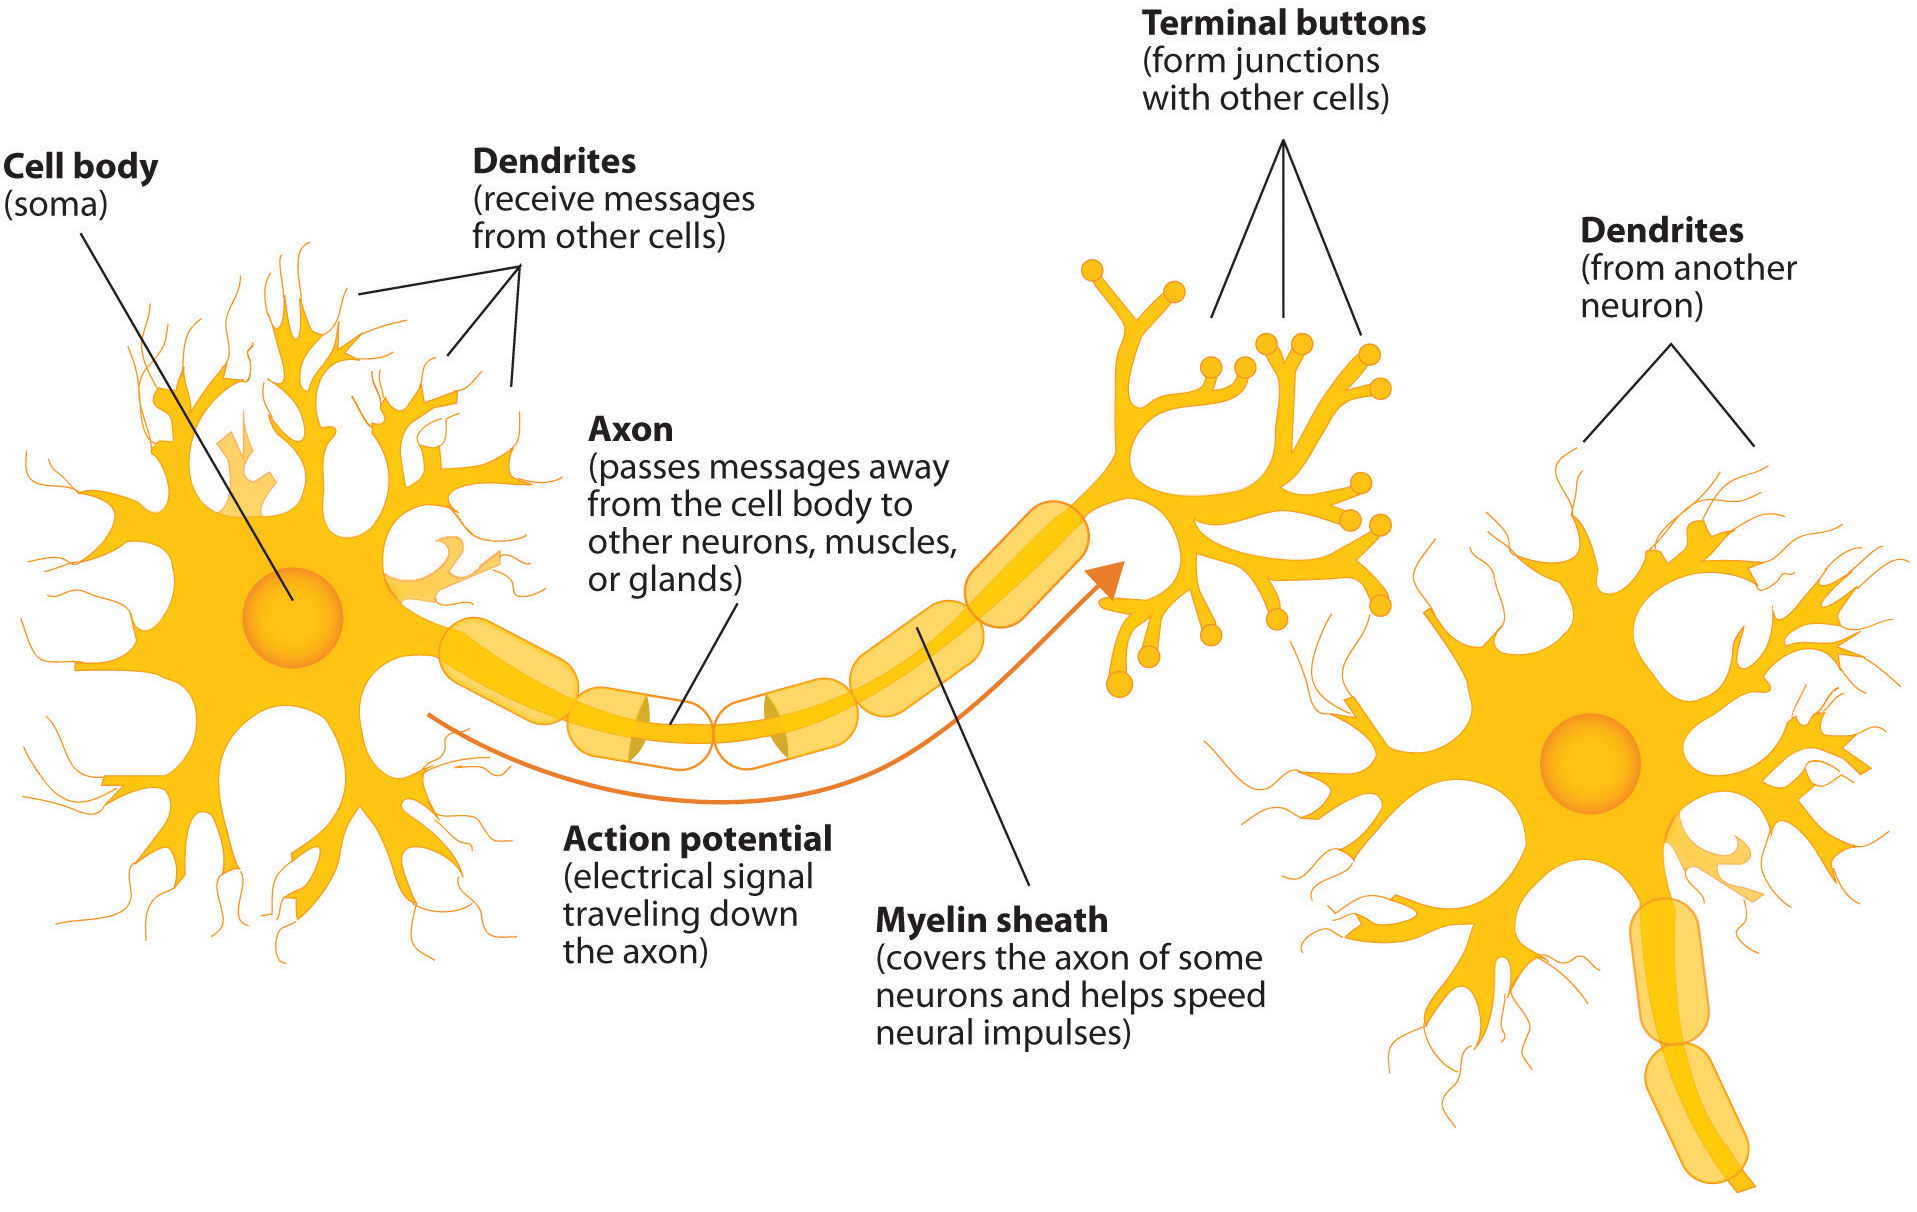
\includegraphics[width=0.99\textwidth]{components_of_neuron}
    \caption[Diagram of the components of a biological neuron]{A Diagram of the components of a biological neuron. The image is from \citeay{wiki_neuron}.}
    \figlbl{components_neuron}
\end{figure}

A biological neuron (c.f. \figref{components_neuron}) is a cell that communicates with other neurons through connections called synapses.
Communication takes place through precisely timed electrical pulses called spikes.
Biological neurons are electrically excitable by voltage changes across their membranes.
If the changes are significant enough within a short interval, the neuron generates a pulse called an action potential.
This action potential travels through the axon and activates synaptic connections.
Other neurons, connected through synapses, receive this signal.
The synaptic signal can be excitatory \sidecite{Takagi_2000} or inhibitory \sidecite{Coombs_Eccles_Fatt_1955}, making the post-synaptic neuron more or less likely to fire an action potential.
Biological neurons can be classified into sensory neurons, motor neurons, and interneurons.
Sensory neurons respond to external stimuli such as light or sound and send signals to the spinal cord or the brain.
Motor neurons receive brain and spinal cord signals to control muscles or organs.
Interneurons connect neurons within the same region of the brain or of the spinal cord.
Multiple connected neurons form a neural circuit.
The neural network in the brain is not static but changes through growth and reorganisation.
This process is referred to as neuroplasticity or neural plasticity \sidecite{Costandi_2016}.

Like a biological neuron, an artificial neuron is connected to other neurons.
Artificial neurons are usually organised in layers that forward signals sequentially.
Although the neurons in the first layer could be considered sensory neurons, the neurons in the last layer could be considered motor neurons, and the neurons in the middle layer could be considered interneurons, such a distinction makes less sense because the artificial neurons function similarly regardless of their layer except for the activation function.
Several variants for artificial neurons have been proposed in the literature. These variants are described in the following  \secref{ann}.
Like biological neurons, multiple artificial neurons are connected to artificial neural networks.


\section{Artificial Neural Networks}\seclbl{ann}
The idea for artificial neural networks (ANN) stems from biology and aims to capture the interaction of biological neurons with a mathematical model.
McCulloch and Pitts proposed the first model for a neuron that can be connected to other neurons in 1943 \sidecite{McCulloch_Pitts_1943}.
Similar to how a neuron of the human brain transmits electrical impulses through the nervous system, the artificial neuron of McCulloch and Pitts receives multiple input signals and transforms them into an output signal.
A neuron takes an input vector $\boldsymbol{x} = (x_1, ..., x_n)$ where $x_i \in \{0, 1\}$ and maps it to an output $\hat{y} \in \{0, 1\}$.
The mapping from the input to the output is done by using an aggregation function $g(\cdot)$ that sums up the input vector $\boldsymbol{x}$ and an activation function $f(\cdot)$ that outputs $1$ if the output of $g(\cdot)$ is bigger than a threshold $\theta$ and $0$ otherwise.
%
\begin{equation}\eqlbl{McCulloch_Pitts_agg}%
	z = g(\boldsymbol{x}) = g(x_1, ..., x_n) = \sum_{i=1}^{n}x_i\\
\end{equation}
%
\begin{equation}\eqlbl{McCulloch_Pitts_act}%
		\hat{y} = f(z) = \begin{cases}
      		1, & \text{if}\ z \geq \theta \\
      		0, & \text{otherwise}
    	\end{cases}
\end{equation}
%
In 1958, \sideciteay{Rosenblatt_1958} developed the Perceptron, which works with real numbers as input.
The input vector $\boldsymbol{x} \in \mathbb{R}^n$ is multiplied with a weight vector $\boldsymbol{w} \in \mathbb{R}^n$ with the same length $n$.
%
\begin{equation}\eqlbl{Perceptron_agg}%
	z = g(\boldsymbol{x}) = g(x_1, ..., x_n) = \sum_{i=1}^{n} w_i \cdot x_i\\
\end{equation}
%
The output $\hat{y} \in \{0, 1\}$ is similar to the McCulloch and Pitts neuron $1$ if the aggregated value is greater than a threshold $\theta$ and $0$ otherwise as described in \eqref{McCulloch_Pitts_act}. With real numbers as input, the equations \eqref*{Perceptron_agg} and \eqref*{McCulloch_Pitts_act} can be rewritten as
%
\begin{equation}\eqlbl{Perceptron}%
		\hat{y} =f(g(\boldsymbol{x})) = \begin{cases}
      		1, & \text{if}\ z - \theta \geq 0 \\
      		0, & \text{otherwise}
    	\end{cases}
\end{equation}
%
Later, the step-function \(f(\cdot)\) was replaced with other functions so that the output can also be a real number \(\hat{y} \in \mathbb{R}\). Often-used activation functions are
%
\begin{equation}\eqlbl{act_functions}%
	\begin{aligned}
		\text{Sigmoid: } & \sigma(z) = \frac{1}{1+\mathrm{e}^{-z}}\\
		\text{Rectified linear unit (ReLU): } & (z)^{+} = \max\{0, z\}\\
		\text{Hyperbolic tangent (tanh): }  & \tanh(z) = \frac{\mathrm{e}^{z}-\mathrm{e}^{-z}}{\mathrm{e}^{z}+\mathrm{e}^{-z}}
	\end{aligned}
\end{equation}
%
By convention, a positive bias $b$ is often used instead of the negative threshold $- \theta$, which leads to:
%
\begin{equation}\eqlbl{nn}%
	z = g(\boldsymbol{x}) = \boldsymbol{w} \cdot \boldsymbol{x} + b = \left( \sum_{i=1}^{n}w_i \cdot x_i \right) + b
\end{equation}
%
The neuron's output is calculated with the activation function of $z$:
%
\begin{equation}\eqlbl{nn2}%
	\hat{y} = f(z)
\end{equation}
%
So far, only the output of a single neuron has been discussed.
However, the brain consists of multiple neurons which are connected through synapses.
Therefore, also ANNs consist not only of one neuron but combine multiple neurons in a network. 
These neurons are organized in layers.
In the simplest case, all neurons from one layer are connected with all neurons of the subsequent layer. This is called a fully connected layer.
For a network with multiple neurons within one layer, the input $\boldsymbol{x}$ is fed into all neurons to obtain $\boldsymbol{\hat{y}}$.
If the layer has $k$ neurons, the output of the aggregation function becomes a vector $\boldsymbol{z} = (z_1, ..., z_k)$. The same applies to the output of the activation function $\boldsymbol{y} = (y_1, ..., y_k)$ and the bias $\boldsymbol{b} = (b_1, ..., b_k)$. The weight vector, on the other hand, becomes a matrix $\boldsymbol{W} = (\boldsymbol{w}_1, ..., \boldsymbol{w}_k)$. For a layer with multiple neurons, \eqref{nn} and \eqref{nn2} can be rewritten with matrix operations:
%
\begin{equation}\eqlbl{nn3}%
	\boldsymbol{z} = \boldsymbol{W} \cdot \boldsymbol{x} + \boldsymbol{b}
\end{equation}
\begin{equation}
	\hat{\boldsymbol{y}} = f(\boldsymbol{z})
\end{equation}
%
which is equal to
%
\begin{equation}\eqlbl{nn4}%
		\boldsymbol{z} = \begin{bmatrix}
			z_1\\
			z_2\\
			...\\
			z_k\\
		\end{bmatrix} = \begin{bmatrix}
			\boldsymbol{w}_1 \cdot \boldsymbol{x} + b_1\\
			\boldsymbol{w}_2 \cdot \boldsymbol{x} + b_2\\
			...\\
			\boldsymbol{w}_k \cdot \boldsymbol{x} + b_k\\
		\end{bmatrix} = \begin{bmatrix}
			\left( \sum_{i=1}^{n}w_{1i} \cdot x_i \right) + b_1\\
			\left( \sum_{i=1}^{n}w_{2i} \cdot x_i \right) + b_2\\
			...\\
			\left( \sum_{i=1}^{n}w_{ki} \cdot x_i \right) + b_k\\
		\end{bmatrix}
\end{equation}
\begin{equation}\eqlbl{nn5}%
		\hat{\boldsymbol{y}} = \begin{bmatrix}
			y_1 = f(z_1)\\
			y_2 = f(z_2)\\
			...\\
			y_k = f(z_k)\\
		\end{bmatrix}
\end{equation}
%

The universal approximation theorem\sidecite{Cybenko_1989} proves that a shallow network with one hidden layer (i.e. one layer between input and output layer) and enough neurons can approximate any mapping function between inputs and outputs.
However, very complex mapping functions may need too many neurons in the hidden layer.
Sequentially arranging multiple layers is much more efficient for approximating complex functions.
A sequential arrangement allows learning a hierarchy of features by dividing the mapping function over several successive processing steps.

In an MLP, the input \(\boldsymbol{x}\) is fed into the first layer, and each subsequent layer \(l\) uses the output of the previous layer \(l-1\) as input.
For a network with \(L\) layers, we denote the layer index as superscript square brackets, i.e. $(\cdot)^{[l]}$.
For example, the weights of layer $l$ are denoted as $\boldsymbol{W}^{[l]}$, the bias as \(\boldsymbol{b}^{[l]}\), the output of the aggregation function as \(\boldsymbol{z}^{[l]}\), and the output of the activation function as \(\boldsymbol{a}^{[l]}\).
The input in the first layer is the input data, i.e. $\boldsymbol{a}^{[0]} = \boldsymbol{x}$, and the output of the last layer is the model's prediction, i.e. $\boldsymbol{a}^{[L]} = \hat{\boldsymbol{y}}$. Thus, the mathematical model of an MLP is defined as

\begin{equation}\eqlbl{mlp}
		\boldsymbol{z}^{[l]} = \boldsymbol{W}^{[l]}\boldsymbol{a}^{[l-1]} + \boldsymbol{b}^{[l]}
\end{equation}
\begin{equation}\eqlbl{mlp2}
		\boldsymbol{a}^{[l]} = f({z}^{[l]})
\end{equation}

So far, only the forward pass used to calculate the output $\boldsymbol{\hat{y}}$ has been discussed.
However, the model output $\boldsymbol{\hat{y}}$ will only be close to the target output $\boldsymbol{y}$ if the weights $\boldsymbol{W}^{[l]}$ and biases $\boldsymbol{b}^{[l]}$ are properly defined in every layer $l$.
These parameters are learned during a training period.
The training can take place in a supervised, semi-supervised, self-supervised (sometimes also called unsupervised), or reinforcement learning setting.
In supervised learning, the output of the model $\boldsymbol{\hat{y}}$ is compared to a given target output $\boldsymbol{y}$.
On the other hand, unsupervised learning tries to find patterns in the input data $\boldsymbol{x}$ and cluster the samples into meaningful groups without using pre-defined target labels. Typically, the target $\boldsymbol{y}$ is derived from the data automatically (e.g. predict a masked part of the data); since the model creates the target by itself, this approach is also called self-supervised.
Semi-supervised learning is a hybrid approach of the aforementioned principles that combines a small amount of labelled data with a large amount of unlabelled data.
Lastly, reinforcement learning algorithms aim to maximize the reward that they receive from an environment based on some action they executed.

These learning principles have in common that a loss function (also called objective function) $\mathcal{L}(\cdot)$ can calculate a loss value based on the model output $\boldsymbol{\hat{y}}$ and the target output ${\hat{y}}$. For example, the mean square error (MSE) can be used for regression problems or the negative log-likelihood for classification problems.
The chosen loss function is minimized iteratively with stochastic gradient descent (SGD)\sidenote{there also exist other optimization algorithms such as SGD with momentum, RMSprop, or Adam \citep{Kingma2015AdamAM}} until the network converges to a (local) minima.
The idea behind stochastic gradient descent is to make use of the fact that the negative gradient of the loss value points to the direction of the steepest descent (i.e. in the direction where the loss becomes smaller).
Therefore, SGD updates the network parameters by taking a step of size $\eta$ toward their negative gradient:
%
\begin{equation}\eqlbl{sgd}
	\begin{aligned}
		\Delta \boldsymbol{W}^{[l]} = & -\eta \cdot \left( \nabla_{\boldsymbol{W}^{[l]}} \mathcal{L} \right)\\
		\boldsymbol{W}^{[l]} \coloneqq & \boldsymbol{W}^{[l]} + \Delta \boldsymbol{W}^{[l]}
	\end{aligned}
\end{equation}
%
and
%	
\begin{equation}\eqlbl{sgd2}	
	\begin{aligned}
		\Delta \boldsymbol{b}^{[l]} = & -\eta \cdot \left( \nabla_{\boldsymbol{b}^{[l]}} \mathcal{L} \right)\\
		\boldsymbol{b}^{[l]} \coloneqq & \boldsymbol{b}^{[l]} + \Delta \boldsymbol{b}^{[l]}
	\end{aligned}
\end{equation}
%
The term $\left( \nabla_{\boldsymbol{W}^{[l]}} \mathcal{L} \right)$ is the gradient of the weights \(\boldsymbol{W}^{[l]}\)  with respect to the loss $\mathcal{L}(\cdot)$ and the term $\left( \nabla_{\boldsymbol{b}^{[l]}} \mathcal{L} \right)$ is the gradient of the bias \(\boldsymbol{b}^{[l]}\)  with respect to $\mathcal{L}(\cdot)$.
The gradients of the weights can efficiently be calculated with an algorithm called backpropagation of error \sidecite{Rumelhart_Hinton_Williams_1986}, which is, in fact, just an intelligent implementation of the chain rule\sidenote{While a detailed discussion on backpropagation is out of scope for this thesis, we refer interested readers to the deep learning course by Andrew Ng \cite{Coursera}}.

One of the most critical design decisions in creating ANNs is how the neurons are connected.
So far, only the case where every neuron of one layer is connected to every neuron of the following layer (so-called fully connected layer) has been described. 
Besides such dense connections, there are several alternatives.
Since this work deals with the processing of visual scenes, the most well-known image-processing network architecture, namely Convolutional Neuronal Networks (CNN), is presented below. This architecture is also primarily used in this thesis. However, various alternative architectures exist for computer vision, such as Vision Transformer (ViT) \sidecite{Dosovitskiy_Beyer_Kolesnikov_Weissenborn_Zhai_Unterthiner_Dehghani_Minderer_Heigold_Gelly_2021} or MLP Mixer \sidecite{tolstikhin2021mlp}, which, however, would go beyond the scope of this introduction to deep learning.























\subsection{Convolutional Networks}\seclbl{cnns}
Convolutional Neural Networks (CNNs) are particularly useful for finding patterns in images but can also be used to analyze non-image data such as audio data or time series.
Similar to FCNs, a CNN is composed of an input layer, an output layer, and many hidden layers in between.
A typical CNN consists of subsequently connected convolutional layers and pooling layers.
Usually, an activation function is applied after each convolutional layer while no activation function is used after pooling layers.
Depending on the task, the last layers can be different, e.g. for image classification the last layers are often fully connected.

Convolutional layers use convolution filters or kernels that slide along input features and create translation-equivariant\sidenote{most CNNs apply downsampling operations to the input and are therefore not translation-invariant but translation-equivariant \cite{Mouton_Myburgh_Davel_2020}} responses known as feature maps \sidecite{Zhang_Itoh_Tanida_Ichioka_1990}.
The size of the filter, which is typically a \(3\times 3\) matrix, determines the size of the receptive field.
The filter is applied to an area of the input, with that area having the same size as the filter.
When applying the filter, the dot product is calculated between the input and the filter and then fed into an output array (i.e. the feature map).
Afterwards, the filter shifts by a stride, repeating the process until the entire input has been processed.
Since only the kernel have to be learned, convolutional layers consists of much less parameters than equivalently sized fully connected layers.
This process of re-using the same weights at different locations of the input is also known as parameter sharing.
As described earlier, multiple convolutional layer can follow on each other.
By doing so, CNNs become hierarchical as the later layers can see the pixels within the receptive fields of prior layers.

Pooling layers reduce the size of the input by conducting dimensionality reduction.
Similar to convolutional layers, a filter slides along the input.
However, this filter does not have any learned parameter but apply an aggregation function.
Usually, the filter either select the pixel with the highest value (max pooling) or calculates the average (average pooling) within the receptive field and forwards it to the output array.
Pooling layers usually discard a lot of information but help to reduce complexity and increase robustness.

In the last decades, various CNN architectures have been proposed, usually consisting of different combinations of CNN and pooling layer.
Further improvements have been achieved by using parallel paths of convolutional layers, batch normalization \sidecite{Ioffe_Szegedy_2015}, and skip connections\sidenote{skip connections skips some of the layers in the network and add the output of a layer to the input of a later layer}.
In this thesis I do not go into these specific architectures but provide some references to some well known architectures; LeNet \sidecite{Lecun_Bottou_Bengio_Haffner_1998}, AlexNet \sidecite{NIPS2012_c399862d}, VGGNet \sidecite{Simonyan_Zisserman_2015}, GoogLeNet \sidecite{Szegedy_Liu_Jia_Sermanet_Reed_Anguelov_Erhan_Vanhoucke_Rabinovich_2014}, ResNet \sidecite{He_Zhang_Ren_Sun_2016}, U-Net \sidecite{Ronneberger_Fischer_Brox_2015}, Mask R-CNN \sidecite{He_Gkioxari_Dollar_Girshick_2017}, SSD \sidecite{Liu_Anguelov_Erhan_Szegedy_Reed_Fu_Berg_2016}, and YOLO \sidecite{Redmon_Divvala_Girshick_Farhadi_2016}.

\subsubsection{Training of Convolutional Neural Networks}\seclbl{train_cnns}
CNNs can be used in various applications such as image recognition, video analysis, natural language processing, anomaly detection in time series and many others.
Since this thesis deals with better representations for visual scenes, this chapter is limited to the typical image analysis tasks; image classification, object detection, and image segmentation.
An overview of these tasks is shown in Figure \figref*{img_analysis_tasks}.
The goal of image classification is to predict an image-level label, i.e. to predict what object is in the image.
A classic example of this problem is predicting whether a cat or a dog is in a picture.
This is typically done for images that only contain one object.
With a multi-label classifier, however, it is also possible to predict whether none, one or several classes are present, i.e. whether a cat, a dog or both are present in the image.
With image classification it is unclear where in the image these objects are located.
Object detection provides a remedy.
The aim of object detection is not only to determine what is visible in the image but also where.
The position of the object is usually indicated by a bounding box (i.e. a rectangle).
Especially when there are several objects within a picture, it is helpful to know which object is where, e.g. that the cat is to the left of the dog.
For some applications, predicting the position with bounding boxes is not sufficient.
In this case, semantic segmentation is often used.
Semantic segmentation is the task where each pixel is classified (the image is divided into segments) which leads to a pixel-wise mask for each object in the image.
This gives us exact information about the shapes of the objects.

\begin{figure}[h]
    \centering
    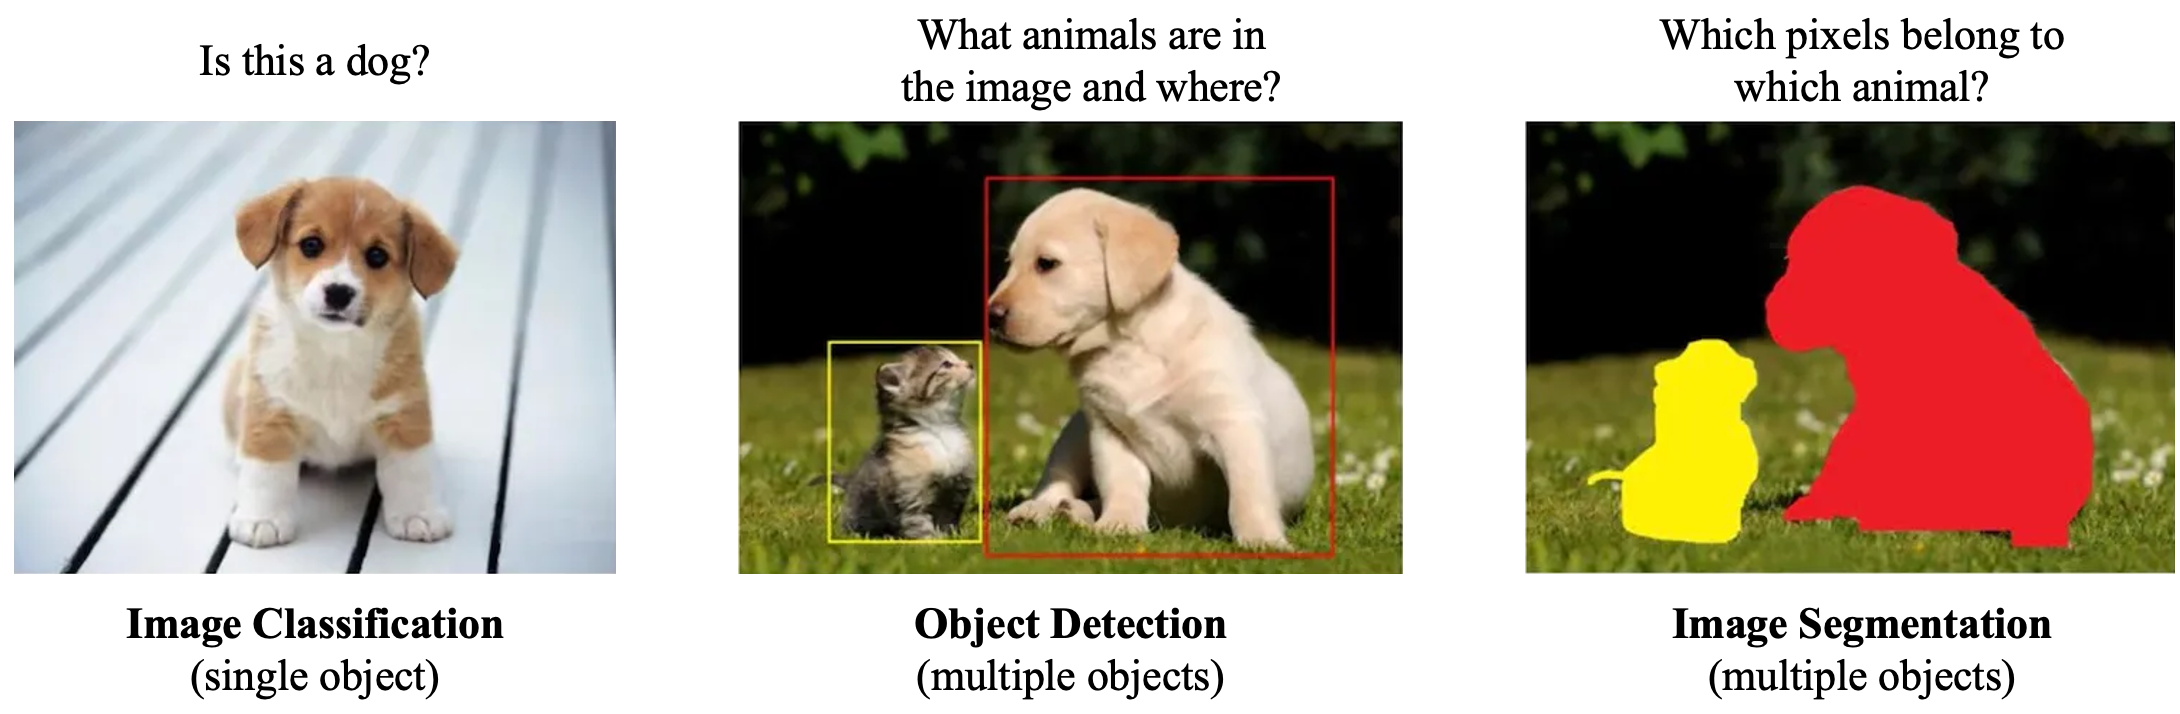
\includegraphics[width=0.99\textwidth]{image_analysis}
    \caption[Overview of different image analysis tasks]{Overview of different image analysis tasks. The image is taken from \citeay{venturebeat_img_analysis} and was slightly adapted.}
    \figlbl{img_analysis_tasks}
\end{figure}


Depending on the task, different kind of labels are required for supervised learning.
Image classification requires labels on image-level (i.e. one or multiple labels per image) \cite{Lecun_Bottou_Bengio_Haffner_1998, NIPS2012_c399862d, Simonyan_Zisserman_2015, Szegedy_Liu_Jia_Sermanet_Reed_Anguelov_Erhan_Vanhoucke_Rabinovich_2014, He_Zhang_Ren_Sun_2016}, object detection requires the coordinates of the bounding box \cite{Redmon_Divvala_Girshick_Farhadi_2016, Liu_Anguelov_Erhan_Szegedy_Reed_Fu_Berg_2016, He_Gkioxari_Dollar_Girshick_2017}, and semantic segmentation requires the labels on pixel-level \cite{Ronneberger_Fischer_Brox_2015, Wu_Zhang_Huang_Liang_Yu_2019} (i.e. each pixel has a label of an object or a label ``background'' for irrelevant pixels).

Besides supervised learning, there are various principles of learning with partial labels or without labels.
These techniques are called weakly-supervised or un-supervised learning and are well summarised in \sidecite{Simmler_Sager_Andermatt_Chavarriaga_Schilling_Rosenthal_Stadelmann_2021}.
Not only specific tasks can be learned, but also task-independent representations.
These representations are typically learned unsupervised\sidenote{also called self-supervised learning because the target labels are derived from the data itself} and can be used for one or several downstream tasks.
More details on visual representation learning are provided in Section \secref*{visual_rep_learning}.
Especially Autoencoders \sidecite{rumelhart1985learning} are explained in this section as they are applied in this thesis.


\section{Limitations}\seclbl{limitationsDL}
The rise of deep learning over the past decade has only been possible because of major technological advances in hardware.
Without the computational resources and the storage capacity of the systems created in the last decades no system could run today's algorithm.
Moreover, much of the progress of recent years was possible due to the improved hardware. 
Moore’s law \cite{Moore_2006} states that the number of transistors in a dense integrated circuit doubles about every two years and is the only known physical process following an exponential curve.
An analysis by OpenAI shows that since 2012 the amount of compute has even increasing exponentially with a doubling time  of \(3.4\) months \cite{OpenAI_compute}.
However, the exponential increase seems to come to an end since the size of transistors hit physical limitations.
It is assumed that Moore's law will end by around 2025 \sidecite{Kumar_2015}.
Besides the progress in the field and the development of new technology, deep learning models also became better because the number of parameters and the size of datasets grew exponentially.
Even the growth in the last five years is astonishing.
While the state-of-the-art language model from 2018 \sidecite{Peters_Neumann_Iyyer_Gardner_Clark_Lee_Zettlemoyer_2018} had around \(94\)M parameters, the state-of-the-art in 2020 \sidecite{NEURIPS2020_1457c0d6} already had \(175\)B parameters. Training such a model on a single V100 GPU would take about 355 years and cost about \(4.6\)M dollars \cite{Lambda_GPT3}.
A recent language model from Microsoft and Nvidia \sidecite{Shoeybi_Patwary_Puri_LeGresley_Casper_Catanzaro_2020} even has \(530\)B parameters.
Only a few institutions with massive resources are able to train such big models.
In general, inference on low-budget hardware such as smartphones or embedded hardware becomes prohibitive with the growing size of deep networks.
Even tough there exist techniques to shrink the model size after training such as quantization \cite{Wu_Judd_Zhang_Isaev_Micikevicius_2020}, model pruning \cite{Choudhary_Mishra_Goswami_Sarangapani_2020}, or model distillation \cite{Hinton_Vinyals_Dean_2015} it is questionable if making models bigger is the best way to develop intelligent systems.

Another major issue of deep learning systems is that they suffer from catastrophic forgetting.
If a model is trained on a specific task and afterwards trained (or fine-tuned) on another task, the model suffers a ``catastrophic'' drop in performance over the first task.
The reason for this effect is that the model during training on the second task adjusts the parameters learned during the first task and therefore ``forgets'' the learned mapping functions.
Just mixing all datasets or to learn all tasks in parallel in a current multi-task setup \cite{Zhang_Yang_2021} doesn't seem feasible to achieve some kind of general intelligence as this involves too many different unrelated tasks.
Catastrophic forgetting is also caused by the fact that learning is mostly done offline\sidenote{Offline in this context means that the model parameters are not adapted after training during inference time}.
Online learning \cite{Sahoo_Pham_Lu_Hoi_2017} and lifelong learning \cite{Parisi_Kemker_Part_Kanan_Wermter_2019} are currently hot research topics.
However, these methods have not yet been established.

Furthermore, there exists problems which may cannot be solved with the current principles used for deep learning.
First of all, it is questionable if deep learning models can achieve \emph{real} generalization\sidenote{Generalization refers to the ability of the model to adapt properly to previously unseen data from the same distribution}.
With enough data, can achieve generalization in the sense that the model can interpolate within the data distribution.
However, deep learning models fail to extrapolate.
For example, convolutional neural networks (CNNs) do not generalize to different viewpoints unless they are added to the training data \sidecite{Madan_Henry_Dozier_Ho_Bhandari_Sasaki_Durand_Pfister_Boix_2022}.

Second, deep learning is not able to learn abstract relationships in a few trials but requires many samples of it and is thus data hungry.\sidenote{Delme!!!}
Marcus Gary \sidecite{Marcus_2018} argues that if he tells that a ``schmister'' is a sister over the age of 10 but under the age of 21, humans can  immediately infer whether they or their best friends have any ``schmister''. However, modern DL systems lacks a mechanism for learning abstractions through explicit, verbal definition and require thousands or even more training samples.

Third, no DL model has been able to demonstrate causal reasoning in a generic way.
Deep learning models find correlations between the inputs and the outputs, but not the causation.
Other AI approaches such as hierarchical Bayesian computing or probabilistic graphical models are better at causal reasoning but cannot be well combined with deep learning models.

Lastly, deep learning models are to some extend too isolated since they have no embodiment and cannot interact with the world.
For example, the human body provides needs, goals, emotions, and gut feeling\sidenote{one could argue that the body is therefore even a co-processor of the brain}.
In current deep learning systems are emotions totally absent and the goals are set externally.
Deep Reinforcement Learning can be considered as a first step in the direction of dissolving this isolation, as they interact with a virtual environment. 
AI systems that interact with the real world do not work well so far.
Moravec's paradox \sidecite{Moravec_1995} states that ``it is comparatively easy to make computers exhibit adult level performance on intelligence tests or playing checkers, and difficult or impossible to give them the skills of a one-year-old when it comes to perception and mobility''.


\section{Biological Learning}\seclbl{biological_learning}
The human brain comprises many interconnected areas processing everything in parallel.
For example, Figure \figref{visual_cortext} illustrates the connections between different organizational units in the cerebral cortex which are responsible for vision.
It can be seen that these areas are connected in a rather complex structure.
\begin{figure}[h]
    \centering
    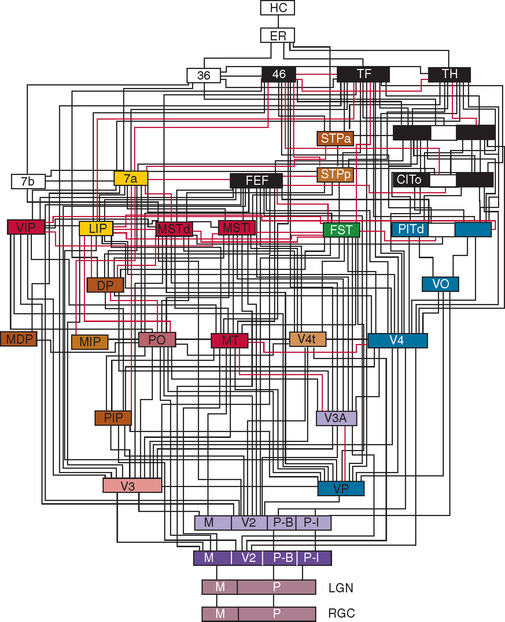
\includegraphics[width=0.99\textwidth]{felleman_visual_cortex}
    \caption[Organization of the visual system in the cerebral cortex]{The organization of the visual system in the cerebral cortex. The image is from \citeay{Felleman_Van_Essen_1991}.}
    \figlbl{visual_cortext}
\end{figure}
Deep learning architectures, on the other hand, are mostly unidirectional and the signal flows unidirectional from layer to layer\sidenote{Except for recurrent connections, skip-connections, or residual-connections}.
However, the choice of the architecture influences the how the model can learn the mapping function from input to output.
It could be that the complex structure of our brain comprises an inductive bias which was learned over time through evolution.

A learning system requires a mechanism that tells the system if something goes well or wrong so that it can learn from it.
This is called the \emph{credit assignment problem}.
Backpropagation (c.f. Section \secref*{fundamentalsDL}) solves this problem by propagating the error backwards through the network.
However, information flows in the brain only in one direction from the presynaptic neurons to the postsynaptic neurons.
Therefore, backpropagation is not biologically plausible.
Lillicrap et al. \sidecite{Lillicrap_Cownden_Tweed_Akerman_2016} shows that an additional set of random feedback weights is able to transmit useful gradients.
Their work has reopend questions how the brain could process error signals and has dispel some long-held assumptions about algorithmic constraints on learning.

Not only the structure of the network and the way how the feedback is calculated is different between biological learning and deep learning.
Also the neurons themselves are different.
While the artificial neuron doesn't have any dynamics (c.f. Equation \eqref*{nn}), biological neurons are highly dynamic:
Biological neurons adapt their firing rate to constant inputs, they may continue firing after an input disappears, and can even fire when no input is active (c.f. Section \secref*{reservoir_comp}).

Lastly, the neurons in the brain are self-organizing.
This means that a group of elementary units such as neurons or a group of neurons perform similar rule of behavior on a sub-set of the available information.
Such a system doesn't have a central supervision that orchestrates these units.
Each unit applies similar deterministic functions to the information received.
Two important principles of such systems are (i) localized learning which means that each unit adapt their behavior to the information they receive; and (ii) emergence which means that there is no explicit loss function that tells the system what to do.


\section{Neurocomputing}\seclbl{neurocomputing}

\subsection{Hebbian Learning}\seclbl{hebbian}
Donald Hebb \sidecite{Hebb_1949} describes how the connections between cells in the nervous system adapt as: ``When an axon of cell A is near enough to excite a cell B and repeatedly or persistently takes part in firing it, some growth process or metabolic change takes place in one or both cells such that A’s efficiency, as one of the cells firing B, is increased''. This statement is often simplified to the well-known phrase ``Neurons that fire together wire together''.

Hebbian learning is based on this principle.
The weight \(w_{ij}\) from neuron \(i\) to neuron \(j\) changes based on the pre-synaptic activity \(r_i\) of neuron \(i\) and post-synaptic activity \(r_j\) of neuron \(j\)

\begin{equation}\eqlbl{hebb_1}
	\Delta w_{ij} = \eta r_i r_j
\end{equation}

where \(\eta\) is the learning rate.
Thus, the weights between frequently co-activated neurons becomes strong which is called Hebbian plasticity.

In its original form, Hebbian learning had the problem that the connections could only become stronger but not weaker.
Therefore, it is often extended based on the covariance of the activity between neurons.
The covariance is positive if two neurons fire often together and negative if they do not often fire together.
The following equation changes the weight relative to the covariance:

\begin{equation}\eqlbl{hebb_2}
	\Delta w_{ij} = \eta (r_i - \psi_i) \cdot (r_j - \psi_j)
\end{equation}

where \(\psi_i\) and \(\psi_j\) are estimates of the expected pre- and post-synaptic activity\sidenote{the expected activity can for example be estimated through a moving average function}.
The formulation above lacks of boundaries, i.e. the weights could grow to infinite.
A simple solution is to enforce hard boundaries \(w_{min} \leq w_{ij} \leq w_{max}\).

Another solution to weaken the connections is given by the Bienenstock-Cooper-Monroe (BCM) learning rule which was introduced by Bienenstock et al. \sidecite{Bienenstock_Cooper_Munro_1982} and extended by Intrator and Cooper \sidecite{Intrator_Cooper_1992}.
They propose a sliding threshold for long-term potentiation (LTP) or long-term depression (LTD) induction.
When a pre-synaptic neuron fires and the post-synaptic neuron is in a lower activity state than the sliding threshold, it tends to undergo a LTD (i.e. the connection is weaken).

Around the same time, Oja \sidecite{Oja_1982} improved the learning rule of Equation \eqref*{hebb_1} with an normalization term:

\begin{equation}\eqlbl{hebb_3}
	\Delta w_{ij} = \eta (r_i r_j - \alpha r^2_j w_{ij})
\end{equation}

The parameter \(\alpha\) is a constant value that determines the size of the norm of the weight vector.
This update rule is also known as the Oja learning rule. 
Furthermore, he has found that a layer of multiple linear neurons converges to the first principle component of the input data.
As all neurons only learn the first principle component, a network of multiple neurons in this setting seem not very useful.
Differentiation between neurons can be achieved with several different methods.
Two well known approaches are the winner-take-all competition (i.e. only the neuron with the most similar activity is selected for learning)\sidenote{in practice is k-winner-take-all often preferred where k instead of one neuron learns} and a recurrent circuit that provides a competitive signal (i.e. the neurons compete with their neighbours to become active to learn).

It is known that independent neurons can encode more information and work better than dependent neurons \sidecite{Simoncelli_Olshausen_2001}.
Anti-Hebbian learning is a method that adds a penalty for similarly active neurons and thus minimizes the linear dependency between neurons.
Vogels et al. implemented this by switching the sign of the weight change \sidecite{Vogels_Sprekeler_Zenke_Clopath_Gerstner_2011}.

There exists many further improvements for Hebbian learning which are not summarized in this thesis.
For example, Joshi and Triesch \sidecite{5178625} as well as Teichmann and Hamker \sidecite{Teichmann} adapt the activation function of the neurons to enforce a certain activity distribution and to stabilize Hebbian learning even in multilayer neural networks.

Similar to large parts of the brain, Hebbian learning is unsupervised and learns based on local information (i.e. neurons in close proximity).
However, the brain is also largely recurrent and could guide neighbouring or preceding units.
This assumption inspired supervised Hebbian learning.
In supervised Hebbian learning, a subset of inputs which should evoke post-synaptic activity can be selected.
Supervised Hebbian learning can be extended to top-down and bottom-up learning \sidecite{Grossberg_1988} which leads to a combination of supervised and unsupervised Hebbian learning.


\subsection{Hopfield Networks}\seclbl{hopfield}
Hopfield networks \sidecite{Hopfield_1982} were introduced 1982 by J. Hopfield.
They serve as associative (i.e. content-adressable) memory systems.
Such systems are particularly useful to retrieve representations based on degraded or partial inputs.
Auto-associative memories return for an input the most similar previously seen sample.
A classical implementation of an auto-associative memory is the nearest neighbour algorithm \sidecite{Fix_Hodges_1989}.
This algorithm compares a given samples with the previously seen training data with a distance metric and returns the most similar sample\sidenote{or the \(k\) most similar samples in the case of the k nearest neighbour (k-NN) algorithm}.
Memory networks \sidecite{Weston_Chopra_Bordes_2015} implement an auto-associative memory within the deep learning framework.
Such networks convert an input \(\boldsymbol{x}\) to a internal feature representation \(I(\boldsymbol{x})\), update memories given the new input \(m=G(m, I(\boldsymbol{x}))\), and compute the output features \(o=O(m, I(\boldsymbol{x}))\).
This process is applied during the training and inference phase.
The only difference is that the parameters for the functions \(I\), \(G\), and \(O\) are only updated during training.

In a Hopfield network are all neurons are connected, but there are no self-connections: \(w_{ii}=0\) where \(w_{ij}\) is the weight between neuron \(i\) and neuron \(j\).
Furthermore, the weights are symmetrical \(w_{ij} = w_{ji}\).
A Hopfield network in its original form works only with binary units.
For consistency, this networks are called binary Hopfield networks in the following.
The output of a neuron in a binary Hopfield network depends on the output of the other neurons within the network:

\begin{equation}\eqlbl{hf_1}
	x_i = \sum_{i \neq j} w_{ij} y_j + b
\end{equation}

\begin{equation}\eqlbl{hf_2}
	y_i = \begin{cases}
      		1, & \text{if} x > 0 \\
      		-1, & \text{otherwise}
    	\end{cases}
\end{equation}

TODO in equation: check where to use y and where to use y with hat


Hopfield networks have their own dynamics and the output evolves over time.
If the initial value \(y_i\) of a binary Hopfield network has a different sign than \(\sum_{i \neq j} w_{ij}y_j + b\) the output will flip (i.e. change its sign).
This will in turn influence all other neurons which may also flip.
The term \(y_i(\sum_{i \neq j} w_{ij}y_j + b)\) is negative if \(y_i\) is not equal to \(\sum_{i \neq j} w_{ij}y_j + b\), otherwise it is positive.
Since the neuron flips if the term \(y_i(\sum_{i \neq j} w_{ij}y_j + b)\) is negative or stays the same if this term is positive, the change of this term can only be positive:

\begin{equation}\eqlbl{hf_3}
	\Delta [y_i(\sum_{i \neq j} w_{ij} y_j + b)] \geq 0
\end{equation}

The negative sum of the term \(y_i(\sum_{i \neq j} w_{ij}y_j + b)\) for the entire network is called the energy \(E\) of the network:

\begin{equation}\eqlbl{hf_4}
	E(\boldsymbol{y}) = -\sum_{i} y_i \left( \sum_{j>i} w_{ji} y_j + b \right)
\end{equation}

As we have shown in \eqref*{hf_3}, the energy function \(E\boldsymbol{y})\) of the network can only decrease.
Moreover, the energy function has a lower bound and thus the network reaches after a finite number of iterations a stable state. 
A stable pattern of the network (i.e. no neurons flip their sign) is a local minima of the energy function and is called a point attractor.
A pattern is attracted by the closest stable pattern.
Thus, the network can be used as associative memory because an input pattern can be matched to the closest stable pattern.

McElice \sidecite{1057328} has shown that a binary Hopfield network with \(N\) neurons has a capacity of \(C=0.138N\) (i.e. the number of patterns that can be stored.
Hebbian learning (c.f. Section \secref*{hebbian}) can be used to store pattern in a Hopfield network.
To store a pattern, the weights \(\boldsymbol{w}\) must be choosen in a way so that the desired local patterns \((\boldsymbol{y}^1, ..., \boldsymbol{y}^P)\) are local minima of the energy function.
By combining Hebbian learning with some smart mathematical transformations it can be shown that the weights can be directly learned with only one iteration over the training patterns\sidenote{for the derivation of this equation refer to \citep{Hopfield_1982}}:

\begin{equation}\eqlbl{hf_5}
	\boldsymbol{w} = \frac{1}{p} \sum_{k=1}^{P} \boldsymbol{y}^k \times (\boldsymbol{y}^k)^T - \boldsymbol{I}
\end{equation}

where \(\boldsymbol{I}\) is the identity matrix.
Later, Hopfield et al. \sidecite{Hopfield1983} extended the binary Hopfield network so that it can either learn pattern during an awake cycle or forget patterns during a sleep cycle.

One of the limiting factors of binary Hopfield networks is the capacity of \(C=0.138N\).
The problems comes from the fact that the energy function is a quadratic function.
More than three decades after the introduction of the binary Hopfield networks, Krotov and Hopfield \sidecite{10.5555/3157096.3157228} reformulated the energy function as a polynomial function to get polynomial capacity \(C\approx N^{a-1}\) where \(a\) is the order of the function.
Later, the energy function was reformulated as exponential function \sidecite{Demircigil_Heusel_Löwe_Upgang_Vermet_2017} and thus modern Hopfield networks have an exponential capacity of \(C\approx 2^{\frac{N}{2}}\).

The second limiting factor of binary Hopfield networks is that only binary patterns can be stored.
Ramsauer et al. \sidecite{Ramsauer} extended the binary Hopfield network to continous patterns by reformulating the energy function and the corresponding update rule.
Continous Hopfield networks can retrieve continous patterns or even combination of several similar continous patterns.
The authors claim that a continous Hopfield networks can replace fully-connected layers, attention layers \cite{10.5555/2969033.2969073}, LSTM layers \cite{Hochreiter_Schmidhuber_1997}, support vector machines (SVM) \cite{Cortes_Vapnik_1995}, and k nearest neighbor (k-NN) \cite{Cover_Hart_1967}.


\subsection{Spiking Neural Networks}\seclbl{spiking_networks}
Biological neurons emit spikes.
To transmit information, especially the firing rate (i.e. the number of spikes per second in Hz) and precise timing of the spikes are relevant.
The amplitude and duration of the spike does not matter much.
This behaviour has also been implemented in ANNs.
So called Spiking neural networks (SNNs) incorporate the concept of time into their model.
SNN do not transmit information in each forward-pass but rather transmit a signal when the membrane potential reaches a threshold value\sidenote{the membrane potential is related to the electrical charge of the membrane of a biological neuron}. 
The neuron fires as soon as the threshold is reached and thereby influences the potential of other neurons.
The most prominent model of a spiking neuron is the leaky integrate-and-fire (LIF) neuron \sidecite{Abbott1999LapicquesIO}.
The LIF neuron models the membrane potential with a differential equation.
Incoming spikes can either increase or decrease the membrane potential.
The membrane potential either decays over time or is reset to a lower value if the threshold value is reached and the neuron has fired.
There exists different integrate-and-fire (IF) neurons models such as the Izhikevich quadratic IF \sidecite{Izhikevich_2003} or the adaptive exponential IF \sidecite{Brette_Gerstner_2005}.
While each of these model gas different mathematical properties, the concept of a membrane potential that is increased or decreased through spikes from other neurons and decays over time or by emitting a spike is similar to the LIF.

Biological neurons have different dynamics.
Some neurons fire regularly if the receive an input current, others slow down the firing rate over time or emits bursts of spikes.
Modern models of spiking neurons can recreate this behaviour of biological neurons \sidecite{Paugam_Moisy}.

The synaptic plasticity can be modeled with Hebbian learning (c.f. Section \secref*{hebbian}).
The spike-timing dependent (STDP) plasticity rule \sidecite{Bi_Poo_2001} distinguishes the tiring behaviour of pre-synaptic and post-synaptic neurons.
If the pre-synaptic neurons fires before the post-synaptic neuron, the connection is strengthen, otherwise it is weaken.

For a long time, SNN only worked for very shallow networks.
In 2018, Kheradpisheh et al. \sidecite{KHERADPISHEH201856} has proposed a SNN based on the idea of CNNs called a deep spiking convolutional network.
This network uses convolutional and pooling layers with IF neurons instead of classical artificial neurones and is trained with STDP.
First, the image is fed into DoG cells.
This cells apply the difference of Gaussians (DoG) feature enhancement algorithm.
This algorithm subtracts a Gaussian blurred version of an image from the original image.
By doing so, positive or negative contrast is detected in the input image.
The higher the contrast is, the stronger is a cell activated and the earlier it emits a spike.
Thus, the order of the spikes depends on the order of the contrast.
These spikes are forwarded to a convolutional layer.
Deep spiking convolutional networks use two types of LIF neurons: On-center neurons fire when a bright area is surrounded by a darker area, off-center neurons do the opposite.
Convolutional neurons emit a spike as soon as they detect their preferred visual feature\sidenote{the location of the feature is not relevant as convolution layers are translation invariant}.
Neurons that fire early perform the STDP update with a winner-takes-all mechanism.
This means that the neurons within a layer compete with each other and those which fire earlier learn the input pattern.
This prevents other neurons from firing and guarantees a sparse connection.
Later convolutional layers detect more complex features by integrating input spikes from the previous layer.
The features from the last convolutional layer are flatten and a Support Vector Machine is used to classify the features.


\subsection{Reservoir Computing}\seclbl{reservoir_comp}
As described in Section \secref*{biological_learning}, biological neurons are highly dynamical while artificial neurons are not.
Reservoir computing introduces such dynamics into an artificial network.
Reservoir computing is an umbrella term for networks based on the concepts of Echo State Networks (ESN) \sidecite{esn} and Liquid State Machines (LSM) \sidecite{Maass_Natschlager_Markram_2002}.
A reservoir is a fixed non-linear system that maps a input vector \(\boldsymbol{x}\) to a higher dimensional computation space.
After the input vector is mapped into computation space, a simple readout mechanism is trained to return the desired output based on the reservoir state.
In principle, the system should be capable of any computation if it has a high enough complexity \sidecite{Konkoli_2018}.
However, not every system is suited as reservoir.
A good reservoir system distributes different inputs into different regions of the computation space \cite{Konkoli_2018}.

A ESN is a set of sparsely connected recurrent neurons as visualized in Figure \figref*{reservoir}.

\begin{figure}[h]
    \centering
    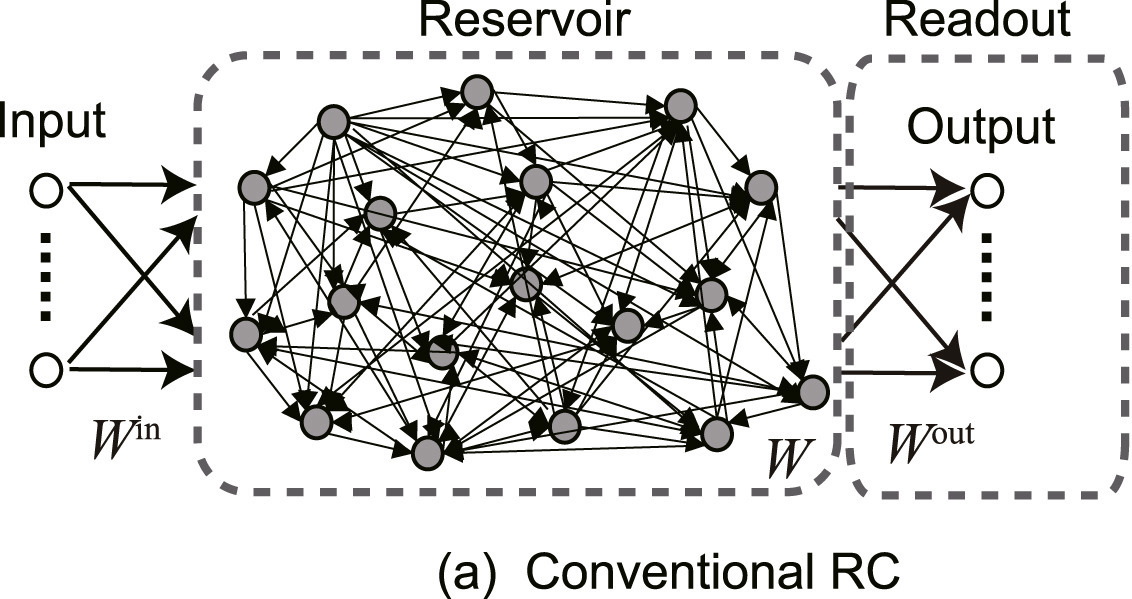
\includegraphics[width=0.99\textwidth]{reservoir}
    \caption[Structure of a Echo State Network]{Structure of a Echo State Network. The image is from \citeay{Tanaka_Yamane_Héroux_Nakane_Kanazawa_Takeda_Numata_Nakano_Hirose_2019}.}
    \figlbl{reservoir}
\end{figure}

The reservoir consists of \(N\) nodes which are connected according a Erdős–Rényi graph model\sidenote{The Erdős–Rényi model is a model for generating random graphs where all graphs on a fixed set of vertices and edges is equally likely} \sidecite{erdos59a}.
This graph model is represented by an adjacency matrix \(\boldsymbol{w}\)\sidenote{Figure \figref*{reservoir} uses upper case letter \(\boldsymbol{W}\)} of size \(N \times N\).
The time varying input signal \(\boldsymbol{x(t)}\) is mapped to a sub-set of \(N/M\) graph nodes by multiplying it with \(\boldsymbol{w}_{\text{in}} \in \mathbb{R}^{N\times M}\) and the output by multiplying the reservoir state with \(\boldsymbol{w}_{\text{out}} \in \mathbb{R}^{M\times N}\).
We refer interested reads to \sidecite{Lukoševičius_2012} to read more about the mathematical properties and how network is updated in detail.

In the original form of ESN, only the readout weights are learned, the rest is chosen randomly.
The input \(\boldsymbol{x(t)}\) brings the recurrent units in a initial state.
The recurrent connections inside the reservoir create different dynamics in the network.
The readout neurons linearly transform the recurrent dynamics into temporal outputs.
The readout weights \(\boldsymbol{w}_{\text{out}}\) are trained to reproduce a target function \(\boldsymbol{y(t)}\).

Liquid State machines use a spiking neural network instead of a graph of recurrent units as reservoir.
The nodes of the spiking neural network are randomly connected together.
Thus, every node receives time varying inputs from the inputs as well as from other nodes.
The recurrent connections turns the varying input into a spatio-temporal pattern.
Similar to ESN, the spatio-temporal patterns of activation are read out by a linear layer.

In general, reservoirs are universal approximators and can approximate any non-linear function given there are enough neurons in the reservoir.
They generalize better and faster than equivalent MLP.
The main drawback of current systems is that cannot deal well with high-dimensional inputs such as images.







\setchapterpreamble[u]{\margintoc}
\chapter{Related Work}\chlbl{rel_work}
%% related_work.tex

\section{Natural Intelligence}\seclbl{natural_intelligence}
This thesis is inspired by the work ''A Theory of Natural Intelligence` from von der Malsburg et al. \sidecite{von_der_Malsburg_Stadelmann_Grewe_2022}.
Therefore, we dedicate this section to summarize their work in detail.

According \cite{von_der_Malsburg_Stadelmann_Grewe_2022}, the process of learning is influenced by ``nature'', ``nurture'', and ``emergence''\sidenote{nature refers to the influence of genes and evolution, nurture to the influence of experience and education}.
They point out that human genome (as of nature) only contain 1GB of information \sidecite{hbcrd} and humans only absorb a few GB into permanent memory over a lifetime (as of nurture) but it requires about 1PB to describe the connectivity in human brain.
Therefore, it is important to distinguish the amount of information to describe a structure from the amount of information needed to generate it.
Similar, nature and nurture only require a few GB to construct, respectively instruct the entire human brain.
Therefore, they argue that the human brain must be highly structured (i.e. nature and nurture ``generate'' the human brain by selecting from a set pre-structured patterns).
The authors call the process of generating the highly structured network in the human brain the ``Kolmogorov \sidecite{Kolmogorov_1998} Algorithm of the Brain''\sidenote{as the Kolmogorov complexity describes the number of bits required by the shortest algorithm that can generate the structure}.
Network self-organization is the only mechanism that has not yet been disproved by experiments as the brains Kolmogorov algorithm \sidecite{Willshaw_VonDerMalsburg_1976, Willshaw_VonDerMalsburg_1979}.
This mechanism loops between activity and connectivity, with activity acting back on connectivity through synaptic plasticity until a steady state, called an attractor network, is reached.
The consistency property of an attractor network means that a network has many alternative signal pathways between pairs of neurons \sidecite{Malsburg_1987}.
Thus, the brain develops as an overlay of attractor networks called net-fragments \sidecite{vonderMalsburg_2018}.
Net-fragments consist of small sets of neurons, whereby each neuron can be part of several net fragments.
The network self-organization has to start from an already established coarse global structure which is improved in a coarse-to-fine manner to avoid being caught in a local optima.

Also, von der Malsburg et al. \cite{von_der_Malsburg_Stadelmann_Grewe_2022} discuss scene representation (i.e. how a scene is represented in the brain) even tough they point out that this is a contested concept \sidecite{freeman1990representations}.
Scene representation is a organization framework to put abstract interpretation of scene layouts, elements, potential actions, and emotional responses in relation.
The details are not rendered as in photographic images but the framework supports the detailed reconstructions of narrow sectors of the scene.
The basic goal if learning is to integrate a behavioral schema into the flow of scene representations.
They propose the hypothesis that the network structure resulting from self-organization together with the neural activation in the framework of scene representation are the inductive bias that tunes the brain to the natural environment.

Finally, they discuss how net fragments can be used to implement such structures and processes using vision as an example.
They point out that a neuron is grouped in one or multiple net fragments through network self-organization.
The net fragments can be considered as filters that detect previously seen patterns in the visual input signal.
An object is represented by multiple net fragments, where each fragment responds to the surface of that object and has shared neurons and connections with other net fragments representing that object.
Thus, net fragments render the topological structure of the surfaces that dominate the environment.
Von der Malsburg et al. \cite{von_der_Malsburg_Stadelmann_Grewe_2022} propose that net fragments represent shape primitives which can adapt to the shape of actual objects\sidenote{adapt in spite of metric deformations, depth rotation, and position}.
Shifter circuits are one possible implementation of networks that enable invariant responses to the position- and shape-variant representations \sidecite{Arathorn_2002, Olshausen1995}.
They are composed of net-fragments that can be formed by network self-organization \sidecite{Fernandes_vonderMalsburg_2015}.
Ref. \cite{von_der_Malsburg_Stadelmann_Grewe_2022} also argue that net fragments are the compositional data structure used by the brain.
A hierarchy of features may be represented by nested net fragments of different size.
Complex objects, such as mental constructs, can thus be seen as larger net fragments composed as mergers of pre-existing smaller net fragments.


\section{Self-Organization}\seclbl{self_org_related}
%% THIS WAS MOVED TO INTRO
%The human brain is self-organizing \sidecite{kelso1995dynamic}.
%Self-organization is the process by which systems consisting of many units spontaneously acquire their structure or function without interference from a external agent or system.
%The absence of a central control unit allow self-organizing systems to quickly adjust to new environmental conditions.
%Additionally, such systems have in-built redundancy with a high degree of robustness as they  are made of many simpler individual units.
%These individual units can even fail without the overall system breaking down.
%Dresp \sidecite{Dresp2020SevenPO} describes seven clearly identified properties of self-organization in the human brain: (i) modular connectivity, (ii) unsupervised learning, (iii) adaptive ability, (iv) functional resiliency, (v) functional plasticity, (vi) from-local-to-global functional organization, and (vii) dynamic system growth.

%Before summarizing the literature specific to self-organization of neural networks, the general literature on self-organization with a focus on deep learning is described in the following.
%Many of these fundamental algorithms for self-organization serve as inspiration for how ANNs can be designed to be self-organizing.

In nature, groups of millions units that solve complex tasks by using only local interactions can be observed.
For example, ants can navigate difficult terrain with a local pheromone-based communication and thus form a collective type of intelligence.
Such observations inspired researchers to build algorithms which are based on local communication and self-organization, for example ant colony optimization algorithms \sidecite{dorigo1997ant}.
DeepSwarm \sidecite{Byla_Pang_2020} is a neural architecture search method that uses this algorithm to search for the best neural architecture.
This methods achieves competitive performance on rather small datasets such as MNIST, Fashion-MNIST, and CIFAR-10.

%Robotic is another research area that uses ideas from collective intelligence such as self-assembly or self-organization.
%For example, swarm systems consist of multiple robots that work together to solve complex tasks \sidecite{Hamann_2018}.
%A famous example of self-assembling robots was presented in 2014 by Rubenstein et al. \sidecite{Rubenstein_Cornejo_Nagpal_2014}.
%They teach kilobots\sidenote{kilobots are 3.3cm tall low-cost swarm robots developed at Harvard University} to self-assemble into target shapes such as letters or stars solely based on local communication between robots.
%However, the kilobots still rely on hand-crafted algorithms to determine their position in the global coordinate system.

%TODO: Write more about swarm intelligence or delete thie paragraph above (does not really fit in here....)

Cellular Automata mimic developmental processes in multi-cell organisms.
They contain a grid of similar cells with an internal state which is updated periodically.
The transition from a given state to a subsequent state is defined by some update rules.
During an update, cells are only allowed to communicate with the neighbouring cells.
Thus, self-organization is enforced by the definition of the update rules.
Such automata can be used to study biological pattern formations \sidecite{Wolfram1984} or physical systems \sidecite{VICHNIAC198496}.
Neural Cellular Automata \sidecite{Wulff1992LearningCA} use neural networks to learn the update rule.
The input in such a neural network is the state of a given cell and its neighbours, the output the subsequent cell state.
Usually, the same network is applied to all cells.
In this case, a fully connected neural network which is applied to each cell and its local neighbours can be reformulated as a CNN\sidecite{PhysRevE}.
NCAs can be trained efficiently with gradient descent to grow given 2D patterns such as images\sidecite{48963, Mordvintsev_Randazzo_Fouts_2022}.
These images are grown through self-organisation (i.e. the pixels pick a color based on the color of neighboring pixels) and are surprisingly resistant to damage.
For example, large parts of the images can be removed and the system is able to rebuild these pixels\sidenote{a demo of this regeneration process is available at \cite{NCAs_distill}}.
However, the aforementioned approaches can only grow the pattern they were trained on.
A recent method called Variational Neural Cellular Automata \sidecite{Palm_GonDuque_Sudhakaran_Risi_2022} use an NCA as decoder of a Variational Autoencoder \sidecite{Kingma_Welling_2014}.
This probabilistic generative model can grow a large variety of images from a given input encoded in a vector format.
However, there is still a big gap in performance compared to state-of-the-art generative models.
Besides growing 2D patterns, NCAs can also create 3D patterns such as buildings in the popular video game Minecraft by utilizing 3D CNNs \sidecite{Sudhakaran_Grbic_Li_Katona_Najarro_Glanois_Risi_2021} or generate structures with specific function such as simulated robots able to locomote\sidecite{Horibe_Walker_Risi_2021}.
Moreover, self-assembling approaches based on NCAs are not restricted to grid-structures.
NCAs can be generalized to graph neural networks \sidecite{Grattarola_Livi_Alippi_2021}.
Graph cellular automata (GCA) use graph neural networks \sidecite{Zhou_Cui_Hu_Zhang_Yang_Liu_Wang_Li_Sun_2021} instead of CNNs to learn the state transition rules and can thus deal with more complex pattern structures than just 2D and 3D grids.
The process of growing images from cells of an NCA can also be inverted.
Randazzo et al. \sidecite{randazzo2020self_classifying} propose to use NCA to classify given structures such as images.
They apply the same network to each pixel and its neighbours of an image.
In an iterative process based on local communication, the image fragments then agree on which object they represent.
NCAs can even be used to control reinforcement learning (RL) agents.
Variengien et al. \sidecite{Variengien_Nichele_Glover_Pontes_Filho_2021} use the observations of the environment as state of the NCA, the subsequent state predicted by the NCA are used as Q-value estimates of a deep Q-learning algorithm \sidecite{Mnih_Kavukcuoglu_Silver_Graves_Antonoglou_Wierstra_Riedmiller_2013}.

Self-organization can not only be used to generate structures but also to optimize the weights of a neural networks over the agents lifetime.
For example, a Hebbian learning rule for meta-learning can be used to self-organize the weights of a RL agent over his lifetime\sidecite{NEURIPS2020_ee23e7ad}.
This means that across multiple episodes the weights of a Hebbian based model are learned.
The weights of the agents policy are reset in every episode and the Hebbian based model is used to update them.
This allows the agent to adapt better to the changed conditions within the environment.

Besides optimizing the weights, self-organization has also been used to change the learning rule itself.
The method ``Evolve and Merge`` \sidecite{Pedersen_Risi_2021} uses the so called ``ABCD'' Hebbian learning rule which updates the weights as follows:
\begin{equation}\eqlbl{McCulloch_Pitts_act}
	\Delta w_{ij} = \alpha (A o_i o_j + B o_i + C o_j + D)
\end{equation}%

$\alpha$ is the learning rate, $o_i$ and $o_j$ are the activity levels of connected neurons and $A$, $B$, $C$, and $D$ are learned constants.
For each connection in the network is one learning rule initialized and the constants are learned.
After a pre-defined number of epochs, the learning rules are clustered and the ones with similar constants are merged.
By repeating this process, the number of parameters can be reduced and robustness increases according to the authors.

Alternatively, it is also possible to initialize the network with shared parameters instead of starting with many rules and merging them over time.
Kirsch and Schmidhuber \sidecite{kirsch2021meta} use multiple tiny recurrent neural networks (RNNs) that have the same weight parameters but different internal states\sidenote{Intuitively, these tiny RNNs can be interpreted as more complex neurons.}.
By using self-organization and Hebbian learning, they show that it is possible to learn powerful learning algorithms such as backpropagation while running the network in forward-mode mode only.
However, it works only for small-scale problems as it can get stuck in local optima.
In general seem self-organizing systems to be hard to optimize and only to work for small datasets or simple problems so far.

Risi \sidecite{risi2021selfassemblingAI} describes why self-organizing systems are hard to train;
First, the system is hard to control because there is no central entity in charge but the system must still be nudges into the right direction.
Second, self-organizing systems are unpredictable (i.e. there exist no mathematical model that tells the outcome of the self-organizing process).

\subsection{Growing Networks}
Unsupervised learning techniques usually map high dimensional input data to a lower-dimensional representation.
One approach to do so are self-organizing maps (SOM) \sidecite{Kohonen_1982, Kohonen_1989}.
They map the input data to a discretized representation of the input space of the training samples, called a map.
In opposite to ANNs, they use competitive learning instead of error correction learning (i.e. back-propagation with gradient descent).
A weight vector is used to map the data to a node in the mapping field.
The datapoints ``compete'' for the weight vectors.
The weight vector of a node in the map that best matches a datapoint is moved closer to that input, as are nodes that are in the neighbourhood.
By doing so, samples that are close in the input space are also closed in the resulting maps.

However, SOM have two major limitations; First, the network structure must be pre-defined which constraints the result mapping accuracy. Second, the capacity of the map is predefined through the number of nodes.
Growing networks are able to overcome this limitations.
Growing networks add nodes or whole layers of nodes into the network structure at the positions of the map where the error is highest.
Many growing networks \sidecite{NIPS1994_d56b9fc4, Reilly_Cooper_Elbaum_1982, Fritzke_1994} add such units after a fixed number of iterations in which the error is accumulated.
After adding a unit, it takes several iterations to accumulate the error again until the next node can be added.

Grow When Required (GWR) networks \sidecite{Marsland_Shapiro_Nehmzow_2002} use a different criterion to add nodes.
Instead of adding nodes to support the node with the highest error, nodes are added when a given input samples cannot be matched with the current nodes by some pre-defined accuracy.
This allows the network to adapt the growing process rather fast; The networks stops growing when the input space is matched b the network with some accuracy and the networks starts growing again if the input distribution changes.

Such GWR networks can be used to build self-organizing architectures.
For example, Mici et al. \sidecite{Mici_Parisi_Wermter_2018} build a self-organizing architecture based on GWR to learn human-object interactions from videos.
They use two GWR in parallel, one to process feature representations of body postures and another to process manipulated objects.
A third GWR is used to combine these two streams and to create action–object mappings in a self-organized manner.
By doing so, they are able to learn human-object interactions and exhibit a model which is more robust to unseen samples than comparable deep learning approaches.


\subsection{Self-Organization in Spiking Neural Networks}\seclbl{self_org_spiking}
Spiking neural networks (SNNs) (c.f. Section \secref{spiking_networks}) communicate through binary signals known as spikes and are very efficient on special event-based hardware\sidecite{8259423}.
There exist several methods to self-organize such architectures.
For the sake of completeness, two well-known approaches are described in the following.
However, since this thesis focuses on self-organization in Deep Learning systems, these approaches are only roughly described and for detailed explanations please refer to the respective literature.

Similar to deep learning, there exists a multitude of different network architectures; Shallow \sidecite{masquelier2007unsupervised, 6469239} and deep networks \sidecite{kheradpisheh2018stdp, mozafari2019bio} structures, fully connected \sidecite{diehl2015unsupervised} and convolutional layers \sidecite{cao2015spiking, tavanaei2016bio}, as well as based on different learning rules such as supervised \sidecite{diehl2015fast, zenke2018superspike}, unsupervised \sidecite{diehl2015unsupervised, ferre2018unsupervised} and reinforcement learning based \sidecite{mozafari2018first}.

A representable method for self-organization in SNNs is proposed by Raghavan et al. \sidecite{Raghavan_Lin_Thomson_2020}.
They introduce a stackable tool-kit to assemble multi-layer neural networks.
This tool-kit is a dynamical system that encapsulates the dynamics of spiking neurons, their interactions as well as the plasticity rules that control the flow of information between layers.
Based on the input, spatio-temporal waves are generated that travel across multiple layers.
A dynamic learning rule tunes the connectivity between layers based on the properties of the waves tiling the layers\sidenote{for more information please refer to \cite{Raghavan_Lin_Thomson_2020}}.

An alternative method proposed by Raghavan and Thomson \sidecite{Raghavan2019NeuralNG} grows a neural network.
They start with a single computational ``cell'' and use a wiring algorithm to generate a pooling architecture in a self-organizing fashion.
The pooling architecture emerges through two processes; First, a layered neural network is grown. Second, self-organization of its inter-layer connections is used to form defined ``pools'' or receptive fields.
They us the Izikhevich neuron model \sidecite{Izhikevich_2003} in the first layer to generate spatio-temporal waves.
The units in the second layer learn the ``underlying'' pattern of activity generated in the first layer. 
Based on the learned patterns, the inter-layer connections are modified to generate a pooling architecture\sidenote{for more information please refer to \cite{Raghavan2019NeuralNG}}.

In general, SNNs have to ``convert'' static input data such as images to a dynamic signal.
For example, images are often converted to such signals by using Difference of Gaussian (DoG) convolution filters \sidecite{Vaila_Chiasson_Saxena_2019, KHERADPISHEH201856}.
Such filters subtract one Gaussian blurred version of an original image from another, less blurred version\sidenote{DoG filter can thus be used to reduce noise and to detect edges}.
This subtraction results in spikes for each pixel.
To encode the filter output into a temporal signal, bigger spikes are forwarded earlier in time than smaller spikes.
However, such approaches lose a lot of information about the input.
For example, in the process described above are all information about color and thin structures lost.
To the author of this thesis, this seems to be the reason why these SNNs can't match the performance of deep learning algorithms so far and often only work well for small gray-scale image-datasets such as MNIST.

\section{Correlation within CNNs}
Self-organization in neural networks can be done based on the input data.
If Hebbian learning is used\sidenote{``Cells that fire together wire together''}, cells are connected based on their correlation (i.e. cells with a high correlation are wired together).
One way to capture the correlation within CNNs are Gram matrices.
Gram matrices are essentially the dot-product between the channels of a feature map and can capture the style of given image.
They are for example used for image style transfer\sidecite{Gatys_Ecker_Bethge_2015} or related fields such as texture synthesis \sidecite{Gatys_Ecker_Bethge_20152}.
Appendix \chref{image_style_transfer} provides an intuitive explanation what image style transfer is and how it is related to Gram matrices.

A Gram matrix can be calculated based on the output of a convolutional layer.
Each filter of a convolutional layer (i.e. each channel) produces a so called convolutional map.
A convolutional map contains information about the content of the image such as object structure and positioning as well as information about the style.
Calculating a Gram matrix eliminates content-related information from the convolutional layer output but does not affect style information (c.f. Appendix \chref{image_style_transfer}).
A Gram matrix calculates the correlations between the convolutional maps (i.e. between the filter responses) of a convolutional layer output.
For a convolutional filter output $F$ of layer $l$ and two flattened convolutional maps $i$ and $j$ it is defined as \sidecite{7780634}:

\begin{equation}\eqlbl{Gram_mat}
		G_{ij}^{l} = \sum_k F^{l}_{ik} \cdot F^{l}_{jk}
\end{equation}%

Thereby, $k$ is a hyperparameter defining how many elements of the convolutional output $F$ are compared.
Gatys et al. \sidecite{7780634} applied this formula the first time to convolutional filters but did not fully explain why it works.
However, they found that the style is captured well in the correlation between convolutional maps.
Later, it was shown \sidecite{10555531720773172198} that matching the Gram matrices between two convolutional filters can be reformulated as minimizing the Maximum Mean Discrepancy (MMD) \sidecite{JMLRv13gretton12a} and thus that the style information is intrinsically represented by the distribution of activations in a CNN.

Intuitively, several filters together can describe the style of the image.
For example, if one filter reacts to vertical white and black lines and a second filter reacts to horizontal white and black lines and the input image has a checkerboard style, then these two filters have a high correlation, which is reflected in the Gram Matrix (c.f. Appendix \chref{image_style_transfer}).

When Hebbian learning is used for self-organization, neurons of filters that often trigger together are connected.
A dataset usually contains specific patterns, which are represented in the Gram Matrix\sidenote{In the following the term pattern is used instead of style, because the Gram matrix can represent not only styles like photorealistic images, drawings, etc., but any non-content related information.
For example, for an animal dataset, one filter could have high activation on white color, a second filter on black vertical lines, and a third filter on black dots.
For a photo of a zebra, the first and second filters would have a high correlation while for a dalmatian, the first and third filters would have a high correlation}.
Thus, neurons are connected that alone represent a certain filter but together represent a certain more complex pattern.


\section{Leveraging Neuroscience for Deep Learning Based Object Recognition}
Prior to this thesis, Lehmann \sidecite{lehmann} examined self-organizing deep learning architectures in Master thesis at the Zurich University of Applied Sciences.
He proposes a new layer called the laterally connected layer (LCL).
The LCL layer extends convolutional layers by forming lateral intra-layer connections based on the Hebbian learning rule (c.f. Section \secref{hebbian}).
Similar to a convolutional filter, the convolutional feature map is calculated.
Afterwards, the convolutional feature maps are compared and the lateral impact between the feature maps is calculated (i.e. how strongly the feature maps influence each other based on their covariance).
When two feature maps are simultaneously in the same pixel locations, their connection strength is increased.
By using Hebbian learning, lateral connections are formed between the feature maps with a high lateral impact.

Lehmann found that LCL layers increase robustness for object recognition.
He shows on the MNIST dataset that for a small reduction in accuracy of 1\%, the performance on corrupted images increases by up to 21\% and that it works especially well for noisy types of corruptions.

\section{Rotation Invariant Convolutions}\seclbl{rotation_invariant_conv}
In this thesis, I show the capability of self-organization to deal with object transformations.
Common transformations of objects in visual scenes are translations, rotations, zooming, and deformations.
While most state-of-the-art architectures are translation invariant\sidenote{STOA architectures for visual scene interpretation are mainly based on convolutional neural networks and vision transformers \cite{Dosovitskiy_Beyer_Kolesnikov_Weissenborn_Zhai_Unterthiner_Dehghani_Minderer_Heigold_Gelly_2021}. These architectures are by definition translation invariant.}, they suffer from the other aforementioned transformations.
The model can be trained to be more robust against most kind of transformations through data augmentation \sidecite{Simard_Steinkraus_Platt_2003}.
For example, dynamically increasing and decreasing image sizes works very well to obtain robustness against different object sizes.
Robustness against deformations, on the other hand, can be learned to a great extend through data pre-processing such as random grid-based deformations \sidecite{Ronneberger_Fischer_Brox_2015, Sager_Salzmann_Burn_Stadelmann_2022}.
However, deformations are often domain specific.
In this thesis, I mainly focus on rotation invariance of visual perception systems as this is a challenging task and is for many applications the most important transformation invariance beyond translation.
Although transformation invariant models can be obtain with data augmentation \cite{Simard_Steinkraus_Platt_2003, Fasel_Gatica_Perez_2006}, this approach is considered inefficient as the model has to learn many redundant parameters, independent for each rotation angle.
In the following, we focus on methods that overcome this limitation.

A simple approach to achieve rotation invariance is to find the main axis of an image patch and to rotate it until it is aligned with the samples from the training set \sidecite{Jafari_Khouzani_Soltanian_Zadeh_2005}.
Another common strategy is to define features that are rotation invariant or equivariant, i.e. to use features whose output is either not affected by rotating the input image or whose output is rotated the same way as the input image by definition.
Some well-known approaches are Local Binary Patterns \sidecite{Ojala_Pietikainen_Maenpaa_2002}, spiral resampling \sidecite{Wen_RongWu_ShiehChungWei_1996}, and steerable pyramid filters \sidecite{greenspan1994rotation}.

Other approaches learn rotatable filters from the input data.
Dieleman et al. \sidecite{Dieleman_DeFauw_Kavukcuoglu_2016} propose four new neural networks blocks.
The probably most important block proposed in their work is a pooling operation that is applied over rotated feature maps to  reduce the number of parameters and to learn rotation invariance more explicitly.
Another approach \sidecite{Laptev_Savinov_Buhmann_Pollefeys_2016} also applies convolutional filters to rotated versions of the image but aggregates the result by taking the maximum activation over the feature maps as output.

Another category of approaches apply rotations to learned convolutional filters.
Earlier approaches \sidecite{Schmidt_Roth_2012, Kivinen_Williams_2011, Sohn_Lee_2012} use a Convolutional Restricted Boltzmann Machine (C-RBM)\sidenote{A C-RBM is a generative stochastic network that can learn a probability distribution over its inputs. Multiple layers of C-RBM are also known as deep belief networks.} \sidecite{Lee_Grosse_Ranganath_Ng_2009} to tie the weights.
Besides using C-RBM, it is also possible to tie the weights within several layers of a CNN to enforce rotation invariance and to reduce the number of parameters to learn. 
Teney and Herbert \sidecite{Teney_Hebert_2016} split the filters of a CNN in orientation groups and constraint their weights.
Such models achieve rotation covariance\sidenote{rotation covariance means that applying a rotation to the input image results in a shift of the output across the features} and only need to learn a single canonical filter per orientation group.
This concept can also be applied to the rotation group in the final layers of a CNN to obtain invariance to global rotations \sidecite{Wu_Hu_Kong_2015}.



%https://numenta.com/htmschool/






TODO: somewhere it is argued that biologically-motivated algorithms work bad: This is shown here: https://arxiv.org/pdf/1807.04587.pdf -> add this as source -> \sidecite{Bartunov_Santoro_Richards_Marris_Hinton_Lillicrap_2018}

\setchapterpreamble[u]{\margintoc}
\chapter{Neuroscientific Concepts}\chlbl{neuro_concepts}
%% neuro_concepts.tex
A large part of the contribution of this thesis consists of identifying appropriate findings from neuroscience and adapting them to a deep learning setting.
The identified concepts and the link between the two disciplines is described in this chapter.
It should be noted that this section presents only one possible interpretation for the implementation of neuroscientific concepts in the context of deep learning and that alternative interpretations might also be promising.
Concrete implementations of the concepts presented in this chapter can be found in \chref{vertical_self_org} and \chref{horizontal_self_org}.


\section{Self-Organisation}\seclbl{neuro_concepts_self_org}
It is known that large parts of the human brain are self-organizing \sidecite{kelso1995dynamic}.
Self-organization is the process by which systems consisting of many units acquire their function through local interaction and without interference from a external supervisory system.
Recently, renowned scientists \sidecite{von_der_Malsburg_Stadelmann_Grewe_2022} put forward the hypothesis that this process of self-organization is \emph{the} key mechanism of natural intelligent systems such as the human brain.
Dresp \sidecite{Dresp2020SevenPO} describes seven clearly identified properties of self-organization in the human brain: (i) modular connectivity, (ii) unsupervised learning, (iii) adaptive ability, (iv) functional resiliency, (v) functional plasticity, (vi) from-local-to-global functional organization, and (vii) dynamic system growth.
However, it is not obvious how these insights from neuroscience can be integrated into a deep learning framework.

Deep learning networks are usually optimized with end-to-end backpropagation of error.
Thus, the entire network is optimized for a specific target.
This is considered a violation of the self-organisation principle, as a global update algorithm (i.e. the optimizer) adjusts all network weights to minimise a global target function.


\begin{claim}
	End-to-end backpropagation of error violates the principle of self-organization. Self-organisation in neural networks requires dividing the network into smaller units that are optimised independently of each other.
\end{claim}

In fact, the plausibility of backpropagation of error for explaining how the brain works was questioned soon after it was published \sidecite{Crick_1989, Grossberg_1987}.
Since then, many alternative and biologically more plausible algorithms have been proposed such as the feedback alignment (FA) algorithm \sidecite{Lillicrap_Cownden_Tweed_Akerman_2014}, generalized recirculation \sidecite{O_Reilly_1996}, as well as target propagation (TP) \sidecite{Le__Cun_1986} (c.f. Section \secref*{alt_train_algo}).
However, Bartunov et al. \sidecite{Bartunov_Santoro_Richards_Marris_Hinton_Lillicrap_2018} have demonstrated that these algorithms do not scale to large vision datasets such as ImageNet \cite{deng2009imagenet} and only work for smaller datasets such as MNIST \cite{MNIST} and CIFAR-10 \cite{cifar_10}.
The only algorithm that seems to scale well is using a proxy objective functions (c.f. Section \secref*{alt_train_algo}).

The biologically most plausible learning algorithm is Hebbian learning (c.f. Section \secref{hebbian}) and its variants such as contrastive Hebbian learning \sidecite{Movellan_1991}.
However, even tough I obtain some promising results in preliminary experiments with Hebbian learning (c.f. Appendix \chref{exp_hebb_learning}), this algorithm doesn't seem to be well suited to learn good image representation if a network is trained from scratch.

Thus, the use of proxy objective functions\sidenote{proxy objective functions are loss functions that are only applied to local units of a system} seems promising; the updates of weights are done in separate local units, yet the power of current deep learning training algorithms can be exploited and systems can be created that can solve complex problems and scale to large datasets by interacting with each other.

\begin{implementation}
	Instead of using end-to-end backpropagation of error to optimise the whole system according to a single global objective function, proxy objective functions are applied to local units. Thus, self-organisation takes place through the optimisation of local units instead of an overall system.
\end{implementation}

The next ambiguity is what local units are in a deep learning setting.
In deep learning models, typically not neurons are modelled but the trainable parameters\sidenote{the weights $\boldsymbol{w}$ and the bias $\boldsymbol{b}$ are modelled, so that the output $y$ can be calculated as $\boldsymbol{y}=\boldsymbol{w} \cdot \boldsymbol{x} + \boldsymbol{b}$ for given data $\boldsymbol{x}$}.
One of the strengths of deep learning systems is that matrix multiplications allow to calculate the layer outputs in one step.
Calculating each neuron activity separately, on the other hand, would be very inefficient.
Therefore, the smallest meaningful unit for local updates seems to be a layer and not a single neuron.
If a neural network is visualised layer-wise from left to right, then the self-organising units line up horizontally. This is why layer-wise self-organisation is also referred to as ``horizontal self-organisation'' in this thesis (c.f. Figure \figref*{horizontal_vertical_self_org}).

\begin{implementation}
	Self-organisation takes place within local units. A local unit can be a part of a model such as layer.
	In this thesis, this type of self-organisation is called horizontal self-organisation.
\end{implementation}

\begin{figure}[h]
    \centering
    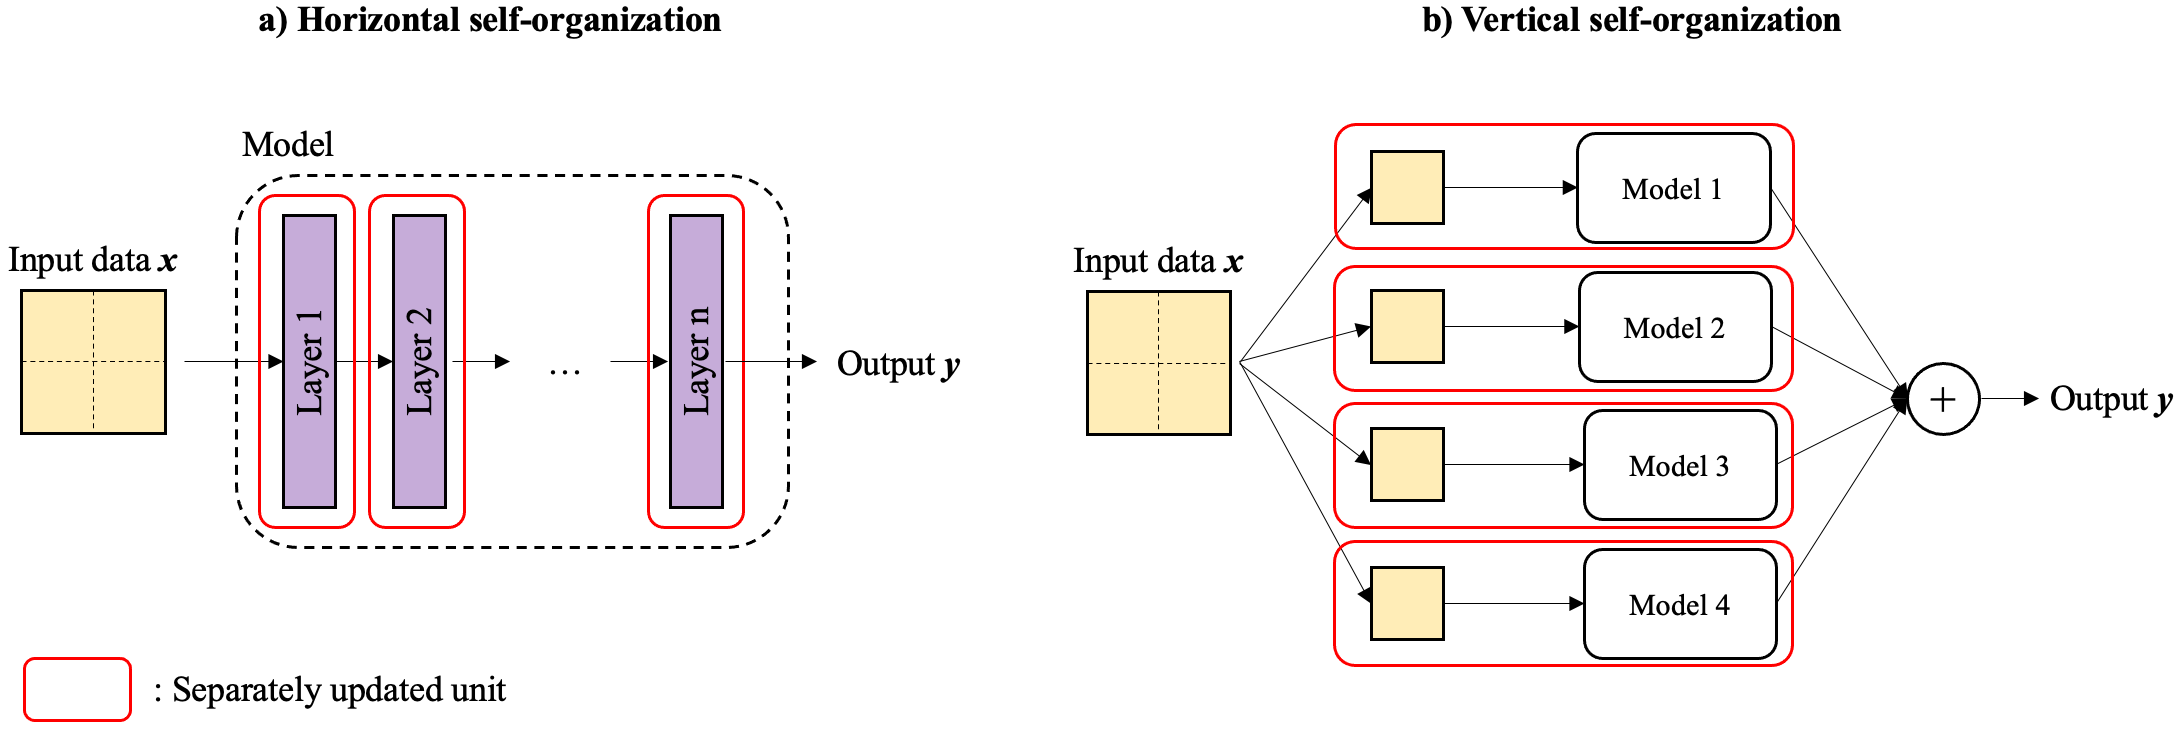
\includegraphics[width=0.99\textwidth]{horizontal_vertical_self_org}
    \caption[Overview of horizontal and vertical self-organization]{Two different ways of building self-organizing units. Self-organization can either take place horizontally (i.e. layer-wise) within a model (a) or vertically by splitting the data into patches and processing them with independent units (b). The independent units are marked with a red frame.}
    \figlbl{horizontal_vertical_self_org}
\end{figure}
 
A second type of self-organisation is not to split the model into separate units but to split the data.
The input data can be divided into smaller patches and then be processed by independent models.
It is important that one model does not process the entire set of existing patches, as is the case with the vision transformer \sidecite{Dosovitskiy_Beyer_Kolesnikov_Weissenborn_Zhai_Unterthiner_Dehghani_Minderer_Heigold_Gelly_2021}. If only one model is used, there would again be an end-to-end backpropagation of error on a single unit.
But if the patches are processed by a graph of independent models, then each model can be considered as a self-organising unit.
In this thesis we call this kind of self-organisation the ``vertical self-organisation'' (c.f. Figure \figref*{horizontal_vertical_self_org}).

\begin{implementation}
	A second type of self-organising unit can be a model that processes a subset of input data that is not shared with other models. In this thesis, this type of self-organisation is called vertical self-organisation.
\end{implementation}


\section{Net-Fragments}\seclbl{neuro_concepts_net_fragments}
Another very important principle according to von der Malsburg et al. \cite{von_der_Malsburg_Stadelmann_Grewe_2022} is that neurons form net-fragments (a.k.a. sub-networks) that represent features of objects (c.f. section \secref{natural_intelligence}).
For example, some net-fragments may represent shapes and structures while a multitude of such net-fragments together represent objects such as persons or entire scenes.
Net fragments are a compositional data structure, meaning that some low-level features can be composed to a higher-level feature and multiple higher-level features are composed to an object.
To some extend, neural networks do this as well; data is fed into the network, the first layer extract some low-level patterns, and subsequent layer combine these patterns in higher-level features in a hierarchical manner.
However, there is one big difference: The features that are used to fulfil a specific task such as classification are extracted from the latent space of \emph{one} single layer.
Net-fragments in the human brain, on the other hand, are not considered to be present at a specific point in time but to be built up over a short period of time.

\begin{claim}
	Net fragments are represented by groups of neurons and their activity over multiple time-dependent spikes. In addition, several net fragments can be composed into a higher-level fragments. Thus, objects are not represented by a single neuron but by all neurons that were activated due to this object.
\end{claim}

Deep learning models are not based on time-dependent spikes of neurons that compose features to more complex features.
However, a time-step could be interpreted as a forward-step from one layer to the next within a network of layers.
Thus, net-fragments would be the activation of multiple layers.
This interpretation is also in line with the compositional property of net-fragments.
Low-level features that are detect within the first layers activate higher-level features in subsequent layers.
An object, however, is not represented in the last layer of a neural network but through all activations within the network.
Thus, representations of objects cannot be extracted from a single layer but from multiple layers.
Intuitively, this seems promising.
For example, auto-regressive models applied on speech capture different information at different layers of the network \sidecite{Chung_Hsu_Tang_Glass_2019}.
While the first layers contain more information to distinguish speakers, representations in later layers provide more phonetic content.
Thus, extracting information from several layers could lead to representations containing more information.

\begin{implementation}
	Net-fragments cannot be extracted from one single layer. Therefore, the representations of an image are extracted from multiple layers.
\end{implementation}

In the human brain, distinct groups of neurons represent specific net fragments.
This means that neurons are only active when the corresponding feature is present in the input and are inactive otherwise.
Moreover, the features represented by the neurons should be meaningful\sidenote{interpretable in the sense that a neuron is active if a specific feature is present and inactive otherwise} and consequently not active for every existing object.
This inevitably leads to the sparse and diverse activations.
The activations are sparse and diverse because, the object in the image consists of only a small sub-set of all learned features. Thus, only a small sub-set of the neurons should be active for a given object.
When the input changes and a different object is shown to the model, also the set of active neurons should change.

\begin{claim}
	The activation patterns of neurons that represent net-fragments must be sparse and diverse to obtain meaningful activation patterns.
\end{claim}

The extent to which neuronal networks contain or can produce net fragments with meaningful activation patterns is investigated in detail in a preliminary study.
The methodology used as well as an in-depth evaluation is described in the appendix in the Chapter \chref{net_fragments}.
In summary, it was found that neural networks do not contain net fragments with meaningful activation patterns by default. Typically, there are neurons that are always active regardless of the input data and encode most of the input information in their activation strength.
Other neurons, however, are never active and are therefore not needed by the network.
If, on the other hand, a sparsity and diversity constraint is applied, then layers are obtained with neurons that appear to be suitable for net fragments.

\begin{implementation}
	Sparse and diverse activation patterns can be obtained by imposing sparsity and diversity constraints to the objective function of the model.
\end{implementation}

However, sparsity and diversity constraints are mainly necessary to obtain meaningful and more robust activation patterns.
They don't seem to be necessary, for example, if the goal is to obtain good classification performance.
An alternative that lead also to robust and meaningful activations is to model the net-fragments as probability distribution.
For example, variational autoencoders (c.f. Section \secref*{visual_rep_learning}) model their latent space as a multivariate Gaussian distribution.

%Especially for models based on horizontal self-organisation, it seems important to impose these constraints on all layers.
%For models with vertical self-organisation, on the other hand, these constraints do not need to be applied to all layers, as long as there are enough models that can only see very small input patches. In this case, a sub-model can only recognise a very spatially-limited feature, which corresponds to a low-level feature. In order to recognise higher-level features or whole objects, interaction with neighbouring sub-models is necessary.
%Thus, net-fragments are composed over several sub-models.
%In this case, it is sufficient to impose the constraints to the function that composes the the representation of the sub-models to higher-level net fragments or to objects.

\subsection{Sparsity}\seclbl{neuro_concepts_sparsity}
Sparistiy seems to be an important principle in biological networks.
Presumably, this is because the neurons in the brain can be inhibitory or excitatory by firing spikes at different time intervals. An artificial neuron, on the other hand, uses a floating point number as its state and can thus represent an infinite number of different states, in contrast to the biological neuron.
Thus, an artificial neuron is able to represent many different things while the biological neuron is responsible for specific features.
Therefore, the activations of biological neurons \emph{must be} sparse, while the activations of artificial neurons \emph{do not have to be} sparse (but being sparse has also advantages for artificial neurons, see below).

Sparsity is deeply embedded in the biological learning process.
For example, in the visual cortex of mice are more than 75\% of the neurons active before the first opening of the eyes, 36\% after the opening of the eyes and only 12\% in adulthood \sidecite{Rochefort_Garaschuk_Milos_Narushima_Marandi_Pichler_Kovalchuk_Konnerth_2009}.
Thus, a sparsification of neuronal activations takes place through visual experience.
In the field of deep learning, sparsity is often interpreted in two different forms; sparse weight matrices and sparse activation matrices.
Sparse weight matrices are often chosen to make models smaller or to increase inference speed \sidecite{Louizos_Welling_Kingma_2018, Hoefler_Alistarh_Ben_Nun_Dryden_Peste_2021}.
From a biological point of view, this process of first creating a large network and then shrinking it is obviously not plausible\sidenote{otherwise we would have a large brain at the beginning, which becomes smaller by factors in the course of time}.
Sparse activations, on the other hand, can increase robustness \cite{Panousis_Chatzis_Theodoridis_2021}.
Intuitively, sparse activations enforce that only the most relevant information is passed to the subsequent layer.
Furthermore, combining sparsity with diversity can help to obtain more interpretable activations (c.f. Appendix Chapter \chref*{net_fragments}).

\section{Lateral Connections}\seclbl{neuro_concepts_lateral_connections}
In addition to forward connections, lateral connections are also located in visual cortex \sidecite{gilbert1990lateral}.
Thus, the biological neurons are not only connected to the neurons in the subsequent layer but also within the same layer.
Von der Malsburg et al. \cite{von_der_Malsburg_Stadelmann_Grewe_2022} describe that lateral connections help active neurons to support each other in order to remain active:
Initially, many neurons are active, but relatively quickly a part of the neuron becomes inactive and only those neurons that support themselves remain active. In this way, lateral connections can lead to the emergence of high-level features from initial activations.

\begin{claim}
	Lateral connections allow active neurons to support each other and to remain active.
\end{claim}


Neural networks lack this time dynamic and neurons do not suddenly become inactive during a forward pass. 
In addition, initial experiments have shown that performance does not improve when the activation maps of neural networks are sparsified over several steps.
One assumption is that all information is already contained in the data at the beginning and the same sparsified activations can also be generated in one initial step.

However, the lateral support between neurons seems promising if the input changes slightly:
An activation map can be calculated for a given input image. In a next step, the input can slightly be changed through data augmentation to btain another activation map from the same image. Thus, the network receives different views of the same image and generates different activation maps of the same image. In every step, the model can decide whether the activation map from the previous step was correct or if the activation map should be updated.

\begin{figure}[h]
    \centering
    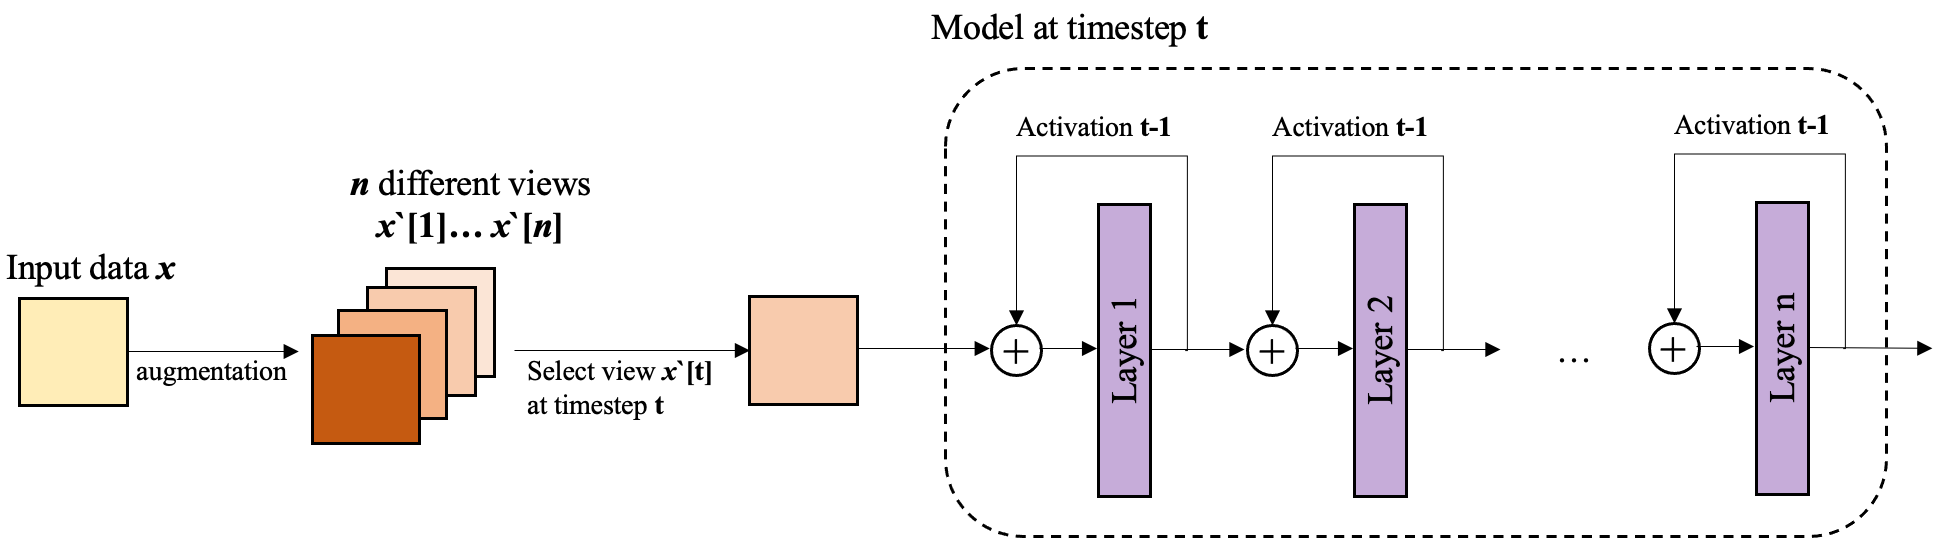
\includegraphics[width=0.99\textwidth]{lateral_connections}
    \caption[Illustrative network architecture of a model with lateral connections]{An illustrative network architecture of a model with lateral connections: An in sample $x$ is augmented $n$ times to obtain $n$ different views $x'[1], ..., x'[n]$ of the same sample. At every timestep $t$, the sample $x'[t]$ is fed through the model. Each layer receives the activation map of the previous layer as input as well as its own activation maps from the previous time-step $t-1$.}
    \figlbl{lateral_connections}
\end{figure}

This could be implemented by interpreting the lateral connection as a recurrent connection.
An illustrative architecture of such a model is shown in Figure \figref{lateral_connections}.
A data sample $x$ can be augmented with data augmentation methods $n$ times to obtain $n$ different views $x'[1], ..., x'[n]$ of the input sample.
Afterwards, the $n$ views are iteratively fed into the model.
At every time-step $t$, the model calculates an activation map $a_l[t]$ for each layer $l$.
If $t>1$, the input of the layer $l$ is not only the activation map of the layer $l-1$ but also the activation map of the previous time-step $a_l[t-1]$.
The activation map of the previous time-step is stored $a_l[t-1]$ by the recurrent (lateral) connection.
Thus, the activation map $a_l[t]$ is not only calculated based on the activation map of the previous layer $a_{l-1}[t]$ but also based on the activation map of the previous time-step $a_l[t-1]$.
This allows each layer to preserve the activation map $a_l[t-1]$ from the previous time-step or to correct it based on a slightly different input $a_{l-1}[t]$ from the previous layer. The lateral connections thus support the activations within a layer; a layer can look at several inputs and decide which features are present over several time-steps (support these features over several time-steps).

\begin{implementation}
	A lateral connection can be implemented as a recurrent connection that ``stores'' the layer's activation of a previous time-step.
	If the same input is present for several time-steps in a slightly augmented version, the layers can keep their previous activation maps (lateral support) or correct them.
\end{implementation}

With vertical self-organisation, the lateral connections can be implemented not only as recurrent connections within layers, but also as connections between the sub-models.
In this case, each sub-model extracts a distinct low-level feature.
Based on this feature, a guess can be made to which higher-level feature or object the extracted feature belongs to.
Through communication with neighbouring sub-models, this guess can either be supported or rejected.
Thus, the lateral connections are used as a ``support channel'' between sub-models. 

\begin{implementation}
	In the case of vertical self-organisation, a lateral connection can be implemented as connection between sub-models to vote for which high-level feature or object is represented in the image. Either the prediction of a model can be supported by neighbouring models or rejected.
\end{implementation}


\section{Other Principles}\seclbl{neuro_concepts_others}
Other important principles that are considered promising are a \emph{continuous input} signal and an \emph{embodiment} of the agent.
However, implementing such an interaction between an agent and an outside world is out of scope for this thesis but might be interesting for future work.

The visual cortex receives a continuous input signal.
This allows the tracking of moving objects and enables an object to be perceived from different angles. Since the change of the object between the captured frames is small, it can be determined that it is always the same object instance and consequently mapped to the same mental object prototype of a world model.

An ANN, on the other hand, is typically trained on samples that have little relation to each other.
When the system is trained on images, each frame is different; with videos, each sequence of frames is different.
A continuous input might help to get better representation of objects through self-supervised learning.
If an input is continuous and shows the same object from different angles or in different transformations (e.g. stretching) and it can be inferred that it is the same object then the object representations derived from this continuous stream can be homogenized.
These principles are already applied to some extent by self-supervised learning systems for computer vision.
In contrastive learning, a popular form of self-supervised learning, two different views are derived from one image by data augmentation, and their representations are then pushed closed together in the feature space \sidecite{chen2020simple, chen2020big, caron2020unsupervised}.
However, this paradigm is still quite limited since only two views of the same scene and not the continuous transformation of an object are presented to the learning system.

\begin{claim}
	A continuous input stream can help to build a better representation of objects, especially if the objects are slightly transformed between captured frames or if the point of view changes continuously and smoothly.
\end{claim}


Furthermore, efference copies of motor signals in the form of neuronal activities are directly sent to the brain’s sensory system if animals are moving \sidecite{Keller_Bonhoeffer_Hübener_2012}.
Such efference copies can be useful to better understand objects and how they behave when undergoing object transformations.
To do so, the agent must be allowed to perform actions and interact with its world.
This gives the agent more information about the objects but also about the physical properties of a (virtual or real) world. For example, he can perform different actions on different objects: He can rotate, squeeze, stretch or move objects. By doing so, he receives different visual and sensory feedback for identical actions on different objects.
The agent can map the captured feedback signals to the object representations of an internal world model.

\begin{claim}
	Allowing an agent to interact with the world can help to learn better object representations and to build a better world model.
\end{claim}

Furthermore, the agent can learn to understand objects better by improving his internal object representations on its own. For example, if the agent examines an object and his current internal object representation does not describe how the object looks from the side, then the agent can rotate the object accordingly and complete or correct the representation. 
Such a behaviour could be implemented within the agent itself, for example, by optimising an entropy-based loss in order that the agent explores the world and tries to learn unknown things \sidecite{storck1995reinforcement, Klapper_Rybicka_Schraudolph_Schmidhuber_2001}.












%TODO: vereinheitliche Mathe: Was ist underline, was ist hochgestellt in Klammern ($z^{(i)}$) und was ist hochgestellt in eckigen Klammern? Bei NN: Was ist n, was ist m, ... (+ Lernraten Symbol, Loss Symbol, etc.)
%Sind alle Vektoren bold?

% TODO: target function und objective function vereinheitlichen
% TODO: net-fragment or net fragment



\setchapterpreamble[u]{\margintoc}
\chapter{Vertical Self-Organisation}\chlbl{vertical_self_org}
%% vertical_self_org.tex
In this thesis, two different concepts of self-organisation are implemented.
This chapter presents a method based on vertical self-organisation (c.f. \secref{neuro_concepts_self_org}).
Vertical self-organisation is based on training small units within a network independent from each other.
The first section presents the methodology (i.e. how vertical self-organisation was implemented), and the second section evaluates the obtained results.


\section{Methods}\seclbl{vertical_self_org_methods}
The first choice for networks based on vertical self-organisation is what the independent units are, i.e. which network parameters are trained independently.
In this thesis, a single layer is used as a self-contained unit. One layer is a small unit (e.g. compared to a model part that contains many layers) but can still be trained efficiently.
Smaller units would be neurons or parts of a layer, but training them separately would be very inefficient since the efficiency of matrix operations on GPUs could no longer be fully exploited\sidenote{the layer output can be efficiently calculated by single matrix multiplication and addition, i.e. $\boldsymbol{z} = \boldsymbol{w} \cdot \boldsymbol{x} + \boldsymbol{b}$ (c.f. \secref{ann})}.

Each layer optimises a proxy objective function.
Proxy objective functions are used because this type of local optimisation allows excellent performance even on larger data sets, in contrast to other local learning algorithms such as target propagation, synthetic gradients or feedback alignment (c.f. \secref{alt_train_algo}). 
 \figref{vertical_gradient_flow} visualises the updates based on a proxy objective function.
An objective function is calculated for each layer, and the optimisation algorithm only updates the parameters within this layer.
Thus, the gradients do not flow back to preceding layers.

\begin{figure}[h]
    \centering
    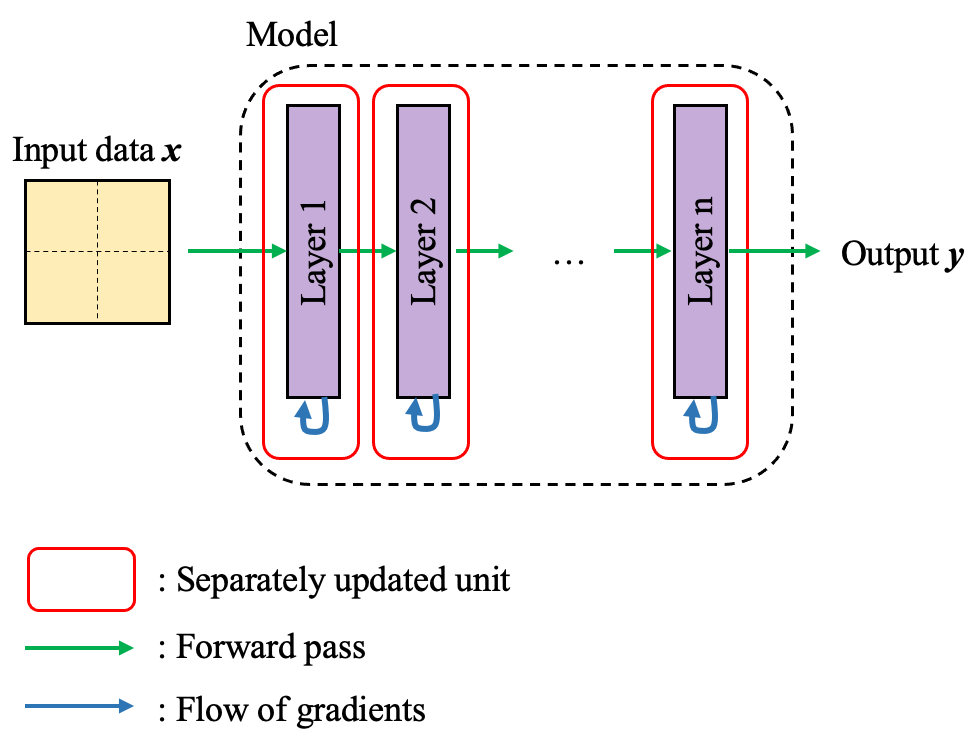
\includegraphics[width=0.99\textwidth]{vertical_gradient_flow}
    \caption[The flow of gradients within the network based on vertical self-organisation]{The flow of gradients within the network based on vertical self-organisation: The data is fed from layer to layer during the forward pass. The layers are trained independently, and the gradients do not flow from one layer to the previous one.}
    \figlbl{vertical_gradient_flow}
\end{figure}

A combination of diversity and sparsity constraints is used as a loss function, which leads to representations that are easy to interpret, suitable for net fragments (c.f. \secref{neuro_concepts_net_fragments}), and also increases robustness (c.f. \secref{neuro_concepts_sparsity}).
Identical to the preliminary experiments in appendix \chref{net_fragments}, the sparsity is achieved by using the kullback-leibler (KL) divergence \sidecite{10-5555-3042573-3042641}.
The model consists of several linear layers $l$ with a ReLU activation function (c.f. \eqref{act_functions}).

A layer consists of $n^{[l]}$ neurons and the activations $\boldsymbol{a}^{[l]}$ of a linear layer $l$ are calculated for a given input $\boldsymbol{a}^{[l-1]}$ as

\begin{equation}\eqlbl{vso_1}
		\boldsymbol{a}^{[l]} = a^{[l]}_1, ..., a^{[l]}_n = \boldsymbol{W}^{[l]} \cdot \boldsymbol{a}^{([l-1]} + \boldsymbol{b}^{[l]}
\end{equation}

whereby $\boldsymbol{W}^{[l]}$ is the weight and $\boldsymbol{b}^{[l]}$ the bias of layer $l$.
The activation probability can be calculated for each neuron. If a mini-batch contains $m$ samples, the activation probability $\hat{\rho}^{[l]}_i$ of a neuron $a^{([l]}_i$ can be calculated as:

\begin{equation}\eqlbl{vso_2}
		\hat{\rho}^{[l]}_i= \frac{1}{n} \sum^n_{i=1} \left( \frac{1}{1+e^{-a^{([l]}_i}} \right)
\end{equation}

where $\left( \frac{1}{1+e^{-a^{([l]}_i}} \right)$ is the sigmoid function that squeezes the activation in the range between $0$ and $1$.
With the KL divergence, the divergence of the current activation probability $\hat{\rho}^{[l]}_i$ and a desired activation probability $\rho=0.05$ can be calculated:

\begin{equation}\eqlbl{vso_3}
		KL(\rho || \hat{\rho}^{[l]}_i) = \rho \cdot \log \frac{\rho}{\hat{\rho}^{[l]}_i} + (1-\rho) \cdot \log \frac{1-\rho}{1-\hat{\rho}^{[l]}_i}
\end{equation}

The sparsity loss $\mathcal{L}^{[l]}_{s}$ of layer $l$ is the sum of the divergence between all $\hat{\rho}^{[l]}_i$ and $\rho$:

\begin{equation}\eqlbl{vso_4}
		\mathcal{L}^{[l]}_{s}(\rho, \hat{\rho}^{[l]}) = \sum_{i=1}^{m} KL(\rho || \hat{\rho}^{[l]}_i)
\end{equation}


The second constraint is a diversity constraint. The goal is that the activations of \emph{different} objects are diverse. For this purpose, the activations $\boldsymbol{a}^{[l]}$ are made as identical as possible (i.e. pushed together in feature space) if they stem from the same class and as different as possible if they stem from different classes.
The cosine similarity is used to calculate the similarity between the activations $\boldsymbol{a}^{[l](i)}$ and $\boldsymbol{a}^{[l](j)}$ of two samples $\boldsymbol{x}^{(i)}$ and $\boldsymbol{x}^{(j)}$:

\begin{equation}\eqlbl{vso_5}
		\text{cos}\left( \boldsymbol{a}^{[l](i)}, \boldsymbol{a}^{[l](j)} \right) = \frac{\boldsymbol{a}^{[l](i)} \cdot \boldsymbol{a}^{[l](j)}}{\max \left( ||\boldsymbol{a}^{[l](i)}||_2, ||\boldsymbol{a}^{[l](j)}||_2 \right)}
\end{equation}

The information of image labels $y^{(i)} \in C$ is needed to push representations of identical objects together or to push representations of different objects apart.
The diversity loss $\mathcal{L}^{[l]}_d$ minimises the similarity $\text{cos} \left(\boldsymbol{a}^{[l](i)}, \boldsymbol{a}^{[l](j)} \right)$ if the activations stem from different classes (i.e. $y^{(i)} \neq y^{(j)}$), or maximises the similarity if they stem from the same class (i.e. $y^{(i)} = y^{(j)}$).

\begin{equation}\eqlbl{vso_6}
		\mathcal{L}^{[l]}_{d} \left(\boldsymbol{a}^{[l]} \right) = \frac{1}{n^2} \sum_{i=1}^{n} \sum_{j=1}^{n} k \cdot \text{cos} \left( \boldsymbol{a}^{[l](i)}, \boldsymbol{a}^{[l](j)} \right) \text{ if } i \neq j
\end{equation}

whereby $k$ changes the sign depending on the class:

\begin{equation}\eqlbl{vso_7}
		k = \begin{cases}
      		+1, & \text{if}\ y_i \neq y_j \\
      		-1, & \text{otherwise}
    	\end{cases}
\end{equation}

However, the loss was found to be more stable if the similarity is not calculated between two activations but between one activation and the average activation of a class. The average activation $\bar{a}[c]$ of a class $c$ can be calculated over $n_c$ samples as:

\begin{equation}\eqlbl{vso_8}
		\bar{a}[c]^{[l]} = \frac{1}{n_c} \sum_{i=1}^{n_c} a^{[l]}_i \text{, for } y_i = c
\end{equation}

Thus, the loss becomes
\begin{equation}\eqlbl{vso_80}
		\mathcal{L}^{[l]}_{d} \left(\boldsymbol{a}^{[l]} \right) = \frac{1}{n\cdot n_c} \sum_{i=1}^{n} \sum_{c \in C} k \cdot \text{cos} \left( \boldsymbol{a}^{[l](i)}, \bar{\boldsymbol{a}[c]}^{[l]} \right)
\end{equation}

Another problem of this loss is that if all activations are identical, then $\text{cos} \left(\boldsymbol{a}^{[l](i)}, \bar{\boldsymbol{a}[c]}^{[l]} \right) = 1$, and the loss becomes $\mathcal{L}^{[l]}_{d}=0$, since the similarities of the same and different classes neutralise each other.
Therefore, a margin between the similarities is enforced, as done for the triplet-margin-loss  \sidecite{Balntas_Riba_Ponsa_Mikolajczyk_2016}.

\begin{equation}\eqlbl{vso_9}
		\mathcal{L}^{[l]}_{d}(\boldsymbol{a}^{[l]}) = \frac{1}{n} \sum_{i=1}^{n} \max \left[ \text{cos}(\boldsymbol{a}^{[l](i)}, \bar{a}[v]^{[l]}) - \text{cos}(\boldsymbol{a}^{[l](i)}, \bar{a}[y^{(i)}]^{[l]}) + \text{margin}, 1 \right]
\end{equation}

where $v$ is a random class drawn from the set $v ~ \{C \\ y_i\}$ and $\text{margin}$ is a hpyer-parameter that was set to $1$.
Thus, the triplet-margin-loss is calculated but the cosine-similarity replaces the $L2$-norm as distance measure and the positive, resp. negative anchor is replaced with the average class activation from the same resp. from a randomly selected different class.

The loss used is the sum of sparsity loss and diversity loss, with the diversity loss weighted by $\lambda=0.1$:
\begin{equation}\eqlbl{vso_10}
		\mathcal{L}^{[l]} =\mathcal{L}^{[l]}_{s}(\rho, \hat{\rho}^{[l]}) 
 + \lambda \cdot \mathcal{L}^{[l]}_{d}(\boldsymbol{a}^{[l]})
\end{equation}


One problem with proxy objective functions is that this type of training often requires layer-wise training. First, layer $1$ is trained until convergence, then the weights are frozen, then layer $2$ is trained and so on.
Such sequential training is inefficient because it requires more forward passes than if the model is trained with end-to-end backpropagation.
It was found that this loss function allows to train all layers simultaneously. With a forward pass, all activations are calculated, followed by a layer-wise backward pass where the gradients from one layer do not propagate back into the previous layer.
Since the gradients are only needed locally, no large graph of gradients has to be calculated, which reduces the memory utilisation on GPUs and allows larger mini-batch sizes. In addition, this type of architecture is straightforward to parallelise since each layer (i.e. each independently trained unit) or a group of layers can be trained on a different GPU:
In contrast to end-to-end backpropagation of error architectures, the gradients only flow backwards locally on a GPU and do not have to be passed on to other GPUs.

\begin{figure}[h]
    \centering
    \resizebox{0.99\textwidth}{!}
{
\begin{tikzpicture}
\tikzstyle{connection}=[ultra thick,every node/.style={sloped,allow upside down},draw=\edgecolor,opacity=0.7]
\tikzstyle{copyconnection}=[ultra thick,every node/.style={sloped,allow upside down},draw={rgb:blue,4;red,1;green,1;black,3},opacity=0.7]


\node[canvas is zy plane at x=0] (input) at (0,0,0) {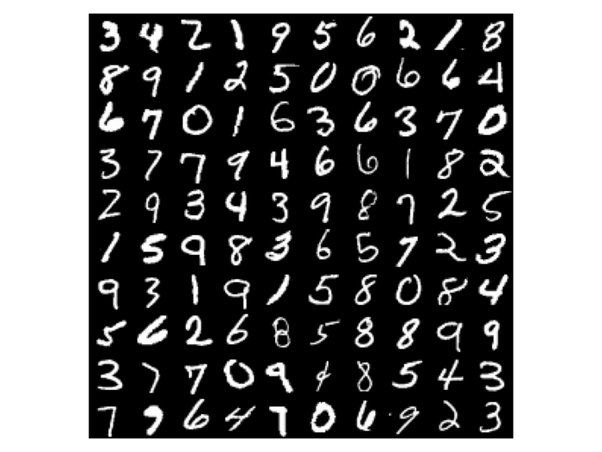
\includegraphics[width=8cm,height=8cm]{imgs/mnist.jpeg}};


\pic[shift={(3,0,0)}] at (input) 
    {Box={
        name=fcn1,
        caption=FC + ReLU,
        xlabel={{" ","dummy"}},
        zlabel=512,
        fill=\SoftmaxColor,
        opacity=0.8,
        height=3,
        width=3,
        depth=52
        }
    };


\draw [connection]  (input) ++(0,0,0)    -- node {\midarrow} (fcn1-west);


\pic[shift={(2,0,0)}] at (fcn1-east) 
    {Box={
        name=fcn2,
        caption=FC + ReLU,
        xlabel={{" ","dummy"}},
        zlabel=256,
        fill=\SoftmaxColor,
        opacity=0.8,
        height=3,
        width=3,
        depth=25
        }
    };


\draw [connection]  (fcn1-east)    -- node {\midarrow} (fcn2-west);


\pic[shift={(2,0,0)}] at (fcn2-east) 
    {Box={
        name=fcn3,
        caption=FC + ReLU,
        xlabel={{" ","dummy"}},
        zlabel=128,
        fill=\SoftmaxColor,
        opacity=0.8,
        height=3,
        width=3,
        depth=13
        }
    };


\draw [connection]  (fcn2-east)    -- node {\midarrow} (fcn3-west);


\pic[shift={(2,0,0)}] at (fcn3-east) 
    {Box={
        name=fcn4,
        caption=FC + ReLU,
        xlabel={{" ","dummy"}},
        zlabel=64,
        fill=\SoftmaxColor,
        opacity=0.8,
        height=3,
        width=3,
        depth=6
        }
    };


\draw [connection]  (fcn3-east)    -- node {\midarrow} (fcn4-west);


\end{tikzpicture}
}
    \caption[Architecture of the fully connected model with vertical self-organisation]{The network architecture of the fully connected model for vertical self-organisation with fully connected layers.}
    \figlbl{vertical_org_arch1}
\end{figure}

The model used consists of $4$ fully connected layers with ReLU activation. The first layer has $512$ neurons, the second $256$ neurons, the third $128$ neurons and the fourth $64$ neurons. The model is illustrated in Figure \figref{vertical_org_arch1}. Each layer is trained separately by minimising the loss of equation \eqref{vso_10} with the Adam optimizer\sidecite{Kingma_Ba_2017} and a learning rate of $\eta = 1 \cdot 10^{-3}$. The mini-batch size is $60,000$. 

\subsection{Extraction of Representations}\seclbl{vertical_self_org_representations}
In accordance with net-fragments as in \secref{neuro_concepts_net_fragments}, the representations are not extracted at a specific point in the network (i.e. a pre-defined layer), but all representations from all layers are taken into account to fulfil a task.
In the following, this is demonstrated based on a classification task, but other tasks are also conceivable in the future.
After training, the average activation $\bar{\boldsymbol{a}[c]}^{[l]}
$ for each class $c \in C$ and layer $l$ is determined, as done in Equation \eqref{vso_8}.
These averages from the training set represent prototypes of each class in each layer and can be considered a reference representation per class. Thus, the representations needed for this task are computed \emph{after} training and are not part of the training as, for example, in the case of a classification loss based on cross-entropy.
When a new sample $\boldsymbol{x}^{(i)}$ is classified, the cosine similarity between the activations $\boldsymbol{a}^{[l](i)}$ of this sample and the class prototypes $\bar{\boldsymbol{a}[c]}^{[l]}$ is calculated in each layer.

\begin{equation}\eqlbl{vso_11}
		\text{cos}[c]^{[l](i)} = \text{cos} \left( \boldsymbol{a}^{[l](i)}, \bar{\boldsymbol{a}[c]}^{[l]} \right) = \frac{\boldsymbol{a}^{[l](i)} \cdot \bar{\boldsymbol{a}[c]}^{[l]}}{\max \left( ||\boldsymbol{a}^{[l](i)}||_2, ||\bar{\boldsymbol{a}[c]}^{[l]}||_2 \right)} \text{, for } c \in C
\end{equation}

Thus, the cosine similarity $\text{cos}[c]^{[l](i)}$ for each class $c \in C$ and each of the layers $l \in {1, ..., 4}$ is calculated. Afterwards, the class $c$ with the highest average cosine similarity between the sample activations $\boldsymbol{a}^{[l](i)}$ and the class prototypes $\bar{\boldsymbol{a}[c]}^{[l]} 
$ is used as prediction.

\begin{equation}\eqlbl{vso_12}
		\argmax_{c \in C} \frac{1}{4} \sum_{l=1}^{4} \text{cos}[c]^{[l](i)}
\end{equation}

This results in a weighted voting; if a layer is certain that the sample belongs to a specific class, the sample has a high cosine similarity with one class prototype and a low similarity with all other class prototypes. Accordingly, this layer influences the prediction more than a layer that cannot assign the sample to one class and calculates a similarly high cosine similarity between the sample and all prototypes.

\subsection{Lateral Connections}
As described in \secref{neuro_concepts_lateral_connections}, lateral connections in the human brain serve neurons to support each other.
There, it is also described that lateral connections can be implemented as recurrent connections.
There are several ways to implement recurrent connections. A straightforward possibility is to concatenate the layer input $\boldsymbol{a}^{[l-1]}[t]$ at time $t$ with the layer output $\boldsymbol{a}^{[l]}[t-1]$  at time $t-1$. This is visualised in \figref{lateral_concat}. Of course, $\boldsymbol{a}^{[l]}[t-1]$ is undefined at $t=0$. In this case, $\boldsymbol{a}^{[l]}[t-1]$ is initialized with zeros.

\begin{figure}[h]
    \centering
    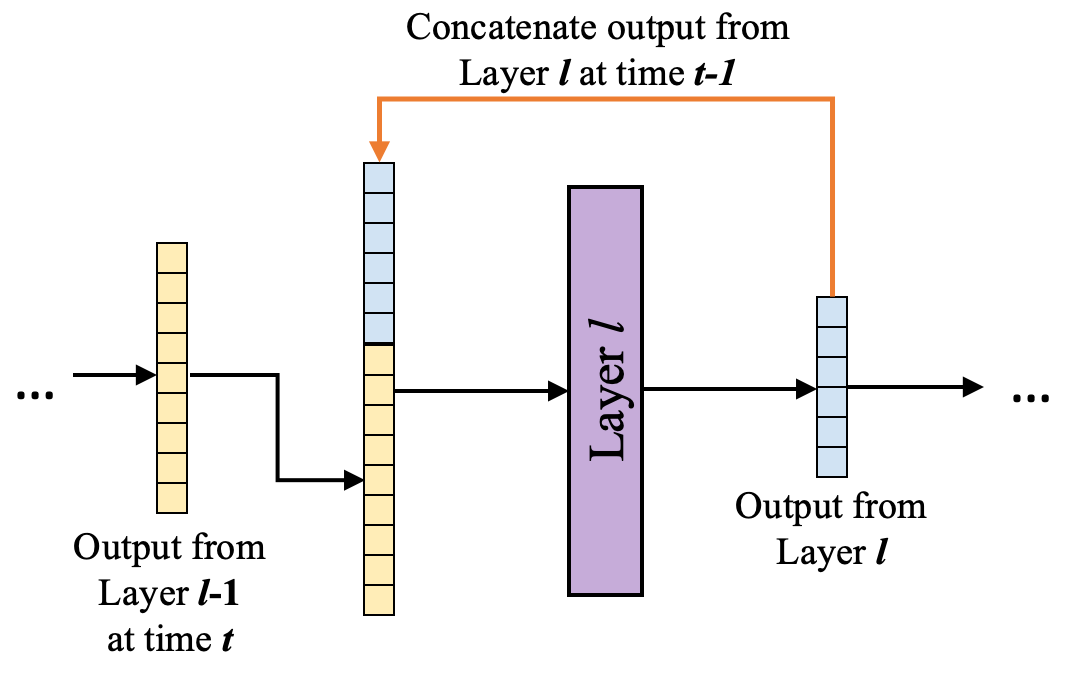
\includegraphics[width=0.99\textwidth]{lateral_concat}
    \caption[Lateral connections by concatenating the layer's output with the layer's input]{The lateral connections can be implemented by concatenating the layer's output at the previous time-step with the layer's input at the current time-step.}
    \figlbl{lateral_concat}
\end{figure}


A second option is to use a second weight matrix, as it is usually done in recurrent layers. Therefore, the equation \eqref{vso_1} is extended as follows:

\begin{equation}\eqlbl{vso_13}
		\boldsymbol{a}^{[l]}[t] =  \boldsymbol{W}_x^{[l]} \cdot \boldsymbol{a}^{[l-1]}[t] + \boldsymbol{b}^{[l]} + \overbrace{\boldsymbol{W}_h^{[l]} \cdot \boldsymbol{a}^{[l]}[t-1] }^{\text{lateral connection}}
\end{equation}

whereby $\boldsymbol{W}_x^{[l]}$ is the weight multiplied with the layer input and $\boldsymbol{W}_h^{[l]}$ the weight multiplied with the previous layer output. In both cases, the layer receives information about the activations at the previous time step.
However, this only seems helpful if the model input is not static. Therefore, the model input is available over several time steps and is augmented after each step. Thus, the model receives different views of the same image and can adjust its activations from the previous time step if necessary. The following image augmentation techniques are applied, each with a probability of $p=0.8$:

\begin{itemize}
	\item \textbf{Color Jitter}: Randomly change brightness, contrast, and saturation of the image.
	\item \textbf{Gaussian Blur}: Blur the image with randomly chosen Gaussian blur.
	\item \textbf{Random Rotation}: Randomly rotate the image with an angle in the range $[-15°, ..., 15°]$
	\item \textbf{Adjust Sharpness}: Randomly adjust the sharpness of the image.
\end{itemize}

\figref{mnist_augmented} visualises how this augmentation affects samples of the MNIST data set \cite{Lecun_Bottou_Bengio_Haffner_1998}. The original image is shown on the left, and $9$ augmented versions of it are shown on the right. This allows the model to perceive the same image from different views.

\begin{figure}[h]
    \centering
    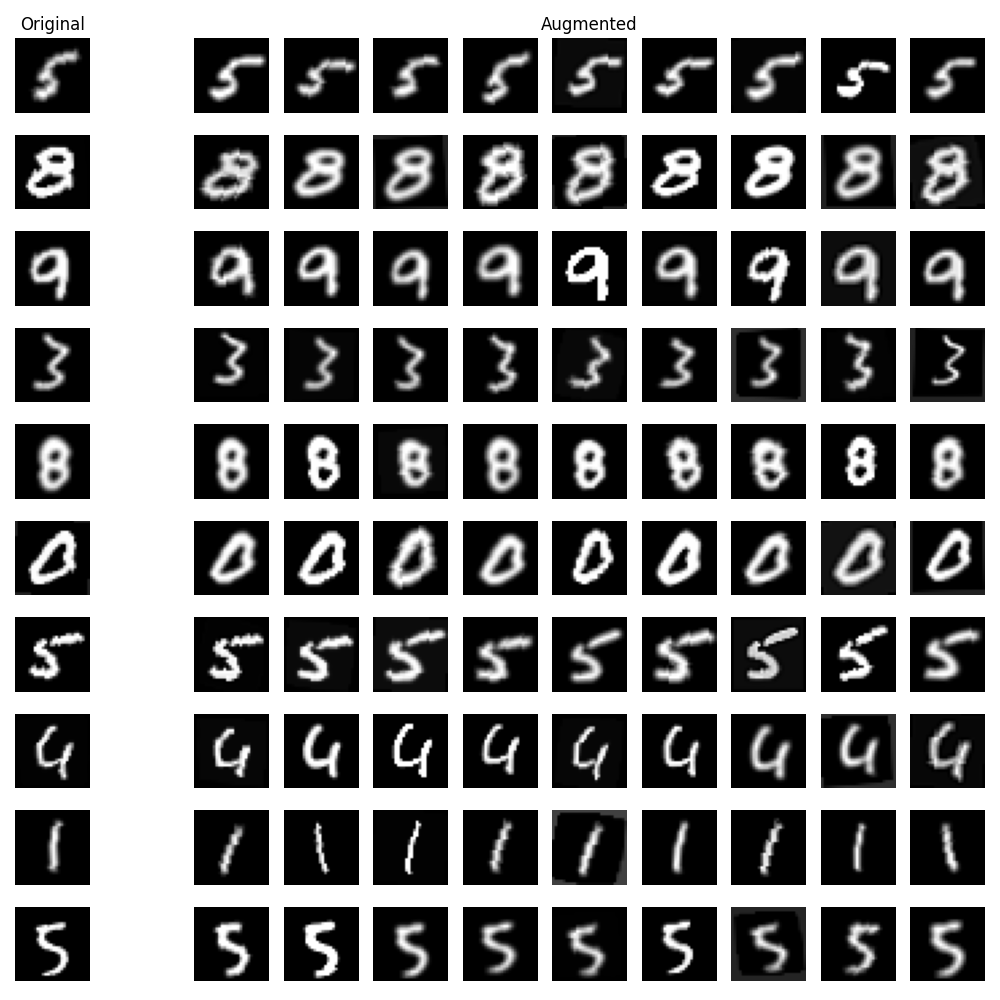
\includegraphics[width=0.99\textwidth]{mnist_augmented}
    \caption[Data augmentation applied on $10$ samples of the MNIST data set]{Data augmentation applied on $10$ samples of the MNIST data set. The original samples from the data set are shown on the left, and $9$ augmented versions of the same samples are shown on the right.}
    \figlbl{mnist_augmented}
\end{figure}


Recurrent connections, which in this context represent lateral connections, are typically used to process sequential data or text. In this case, the data is collected cumulatively before an output is generated. For example, in text processing, all word tokens of a sentence are typically read before the model classifies a sentence. This is necessary because all information is required, and classification cannot be done on the basis of a single token. Such models are typically trained with backpropagation through time (BTT). Thereby, the gradients flow backwards over several time steps. This leads to well-known problems such as vanishing and exploding gradients.

In this thesis, BTT is not used, which means that a prediction is made after each time step, but the prediction potentially improves with more time steps. This leads to desirable properties: (i) Problems with vanishing or exploding gradients do not exist, regardless of how many time steps the model requires. (ii) After each time step, representations can be extracted according to \secref{vertical_self_org_representations}. If an object representation can be assigned to one class label with a high probability, the sequential processing of different image views can be aborted. If this is not the case, further time steps can be carried out until the model has sufficiently high confidence in its prediction. Thus, the number of time steps can be sample-dependent.


% Idee: Mehr Robustheit indem z.b. in einem timestep noise als Input genutzt wird oder bei 1 von 10 timesteps (ausser in den ersten 2) das Bild zufälligerweise vertauscht wird. -> Lateral connections should help

\subsection{Hierarchical Features}\seclbl{vertical_self_org_hierarchical_features}
A criticism of the proposed model is that it does not learn hierarchical features, even though hierarchical features are one of the main reasons for the excellent performance of deep learning systems. The diversity loss (c.f. \eqref{vso_9})  enforces in each layer that the latent representations of objects of the same class are similar and that the representations of different classes are different. This violates the concept of hierarchical features; the first layers should learn general features that are helpful for all classes but cannot necessarily be assigned to a specific class. Only later layers build class representations that are specific to a class. In the current setting, however, already the first layers generate class-specific representations.

In the following, three possible measures are described to counteract this problem: (i) The fully connected layers are replaced by convolutional layers so that the first layers have a smaller field of view and can only recognise local features. (ii) An adapted version of the diversity loss enforces a separation of features by class only in the last layers. (iii) While specific information in the form of the input image flows into the network from one side, general information in the form of class labels is fed into the network from the other side, and these two types of information are fused. Thus, the training process enforces a hierarchy by fusing specific and general information over multiple layers.
These three measures can be applied either individually or in combination with each other.


\subsubsection{Convolutional Architecture}
In a CNN, the field of view in the first layers is restricted by design but becomes larger in subsequent layers. Consequently, using a CNN architecture instead of a model based on fully connected layers alleviates the problem of non-hierarchical features.


\begin{figure}[h]
    \centering
    \resizebox{0.99\textwidth}{!}
{
\begin{tikzpicture}
\tikzstyle{connection}=[ultra thick,every node/.style={sloped,allow upside down},draw=\edgecolor,opacity=0.7]
\tikzstyle{copyconnection}=[ultra thick,every node/.style={sloped,allow upside down},draw={rgb:blue,4;red,1;green,1;black,3},opacity=0.7]


\node[canvas is zy plane at x=0] (input) at (0,0,0) {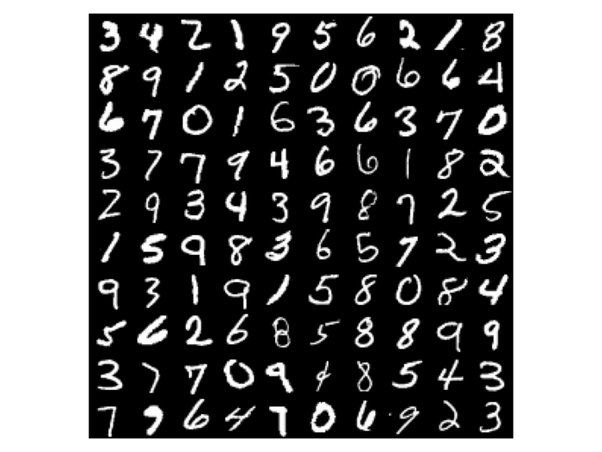
\includegraphics[width=8cm,height=8cm]{imgs/mnist.jpeg}};


\pic[shift={(3,0,0)}] at (input) 
    {Box={
        name=conv1,
        caption=Conv + ReLU,
        xlabel={{1, }},
        zlabel=16,
        fill=\ConvColor,
        height=16,
        width=2,
        depth=16
        }
    };


\draw [connection]  (input) ++(0,0,0)    -- node {\midarrow} (conv1-west);


\pic[shift={ (0,0,0) }] at (conv1-east) 
    {Box={
        name=pool1,
        caption= ,
        fill=\PoolColor,
        opacity=0.5,
        height=8,
        width=1,
        depth=8
        }
    };


\pic[shift={(2,0,0)}] at (pool1-east) 
    {Box={
        name=conv2,
        caption=Conv + ReLU,
        xlabel={{16, }},
        zlabel=32,
        fill=\ConvColor,
        height=8,
        width=4,
        depth=8
        }
    };


\draw [connection]  (pool1-east)    -- node {\midarrow} (conv2-west);


\pic[shift={ (0,0,0) }] at (conv2-east) 
    {Box={
        name=pool2,
        caption= ,
        fill=\PoolColor,
        opacity=0.5,
        height=4,
        width=1,
        depth=4
        }
    };


\pic[shift={(2,0,0)}] at (pool2-east) 
    {Box={
        name=conv3,
        caption=Conv + ReLU,
        xlabel={{32, }},
        zlabel=64,
        fill=\ConvColor,
        height=4,
        width=6,
        depth=4
        }
    };


\draw [connection]  (pool2-east)    -- node {\midarrow} (conv3-west);


\end{tikzpicture}
}
    \caption[Architecture of the CNN for vertical self-organisation]{The network architecture of the CNN for vertical self-organisation with fully connected layers.}
    \figlbl{vertical_org_arch2}
\end{figure}

The CNN architecture used in this thesis is shown in \figref{vertical_org_arch2}.
Three convolutional layers with ReLU activation functions and with $16$, $32$, and $64$ channels are used, and max-pooling layers are applied between each convolutional layer. For training, the same hyperparameters and loss functions are used as for the model with fully connected layers.

\subsubsection{Hierarchical Diversity Loss}
A second measure to obtain hierarchical features is to adapt the diversity constraint of the loss function. The current version forces the latent representations of objects of the same class to be similar and those of different classes to be different. This is useful in the last layers, where high-level features (i.e. high-level net fragments) or object representations should be detected and separated from each other. In the first layers, on the other hand, the separation should not depend on the class label. Nevertheless, the activations should also be diverse if low-level features are detected (c.f. Section \secref{neuro_concepts_net_fragments}).

Therefore, the sparsity constraint is split into two parts: One part ensures that the activations within a (large) mini-batch are diverse and thus enforces that different features are captured and represented by different neurons. The second part ensures, as before, that the activations are diverse for different classes. Thus, one part of the constraint ensures \emph{diversity within the mini-batch} and the other part ensures \emph{diversity between different classes}.

These two parts are weighted linearly from the first to the last layer. Since the first layer should have a high diversity within the mini-batch, it has a high weight on the first part of the diversity constraint and a low weight on the second part. The last layer has an inverse weighting and pays more attention to the diversity constraint's second part than the first part.

The first part of the diversity constraints ensures diversity within a mini-batch. This is achieved by ensuring that each neuron within a mini-batch should be active. 

TODO: At the moment, various experiments are still ongoing to find out how this can be implemented (therefore, not yet explained in more detail).


\subsubsection{Two-Way Information Flow}
Hinton \sidecite{ff_algo} introduced with the forward-forward (FF) algorithm (c.f. Section \secref{alt_train_algo}) a promising idea for models based on proxy objective functions: 
The image is fed into the input layer of the network, and the corresponding label is fed into the output layer of the network. The image remains static for several time steps, and the network is trained to push the layer's activations above a certain threshold. In a second stage, the image is fed into the network with the wrong label and the network is trained to push the activations below a certain threshold. He found that a feature hierarchy is created when low-level features (i.e. images) are fed into the network from one end and high-level features (i.e. class labels) are fed into the network from the other end. However, this approach has one major disadvantage: During inference, each possible sample-label combination has to be fed into the model, and the label that caused the highest neural activity is used as the model's prediction.

In this thesis, this is implemented in a different way, which does not have this disadvantage. Identical to the FF algorithm, the image is fed into the network's input layer for multiple time steps. Conversely, the label is not fed directly into the output layer but is made available to the last layer within the loss function. Each layer maximises the mutual information (MI) between its activations and the activations of the previous and subsequent layers. Thus, the first layer maximises the MI between the input image and its activations, the last layer maximises the MI between its activations and a label vector. This creates a feature pyramid in which a smooth transition from concrete samples to abstract class labels is learned. During inference, the last layer directly predicts latent representations that can be assigned to a class.

\begin{figure}[h]
    \centering
    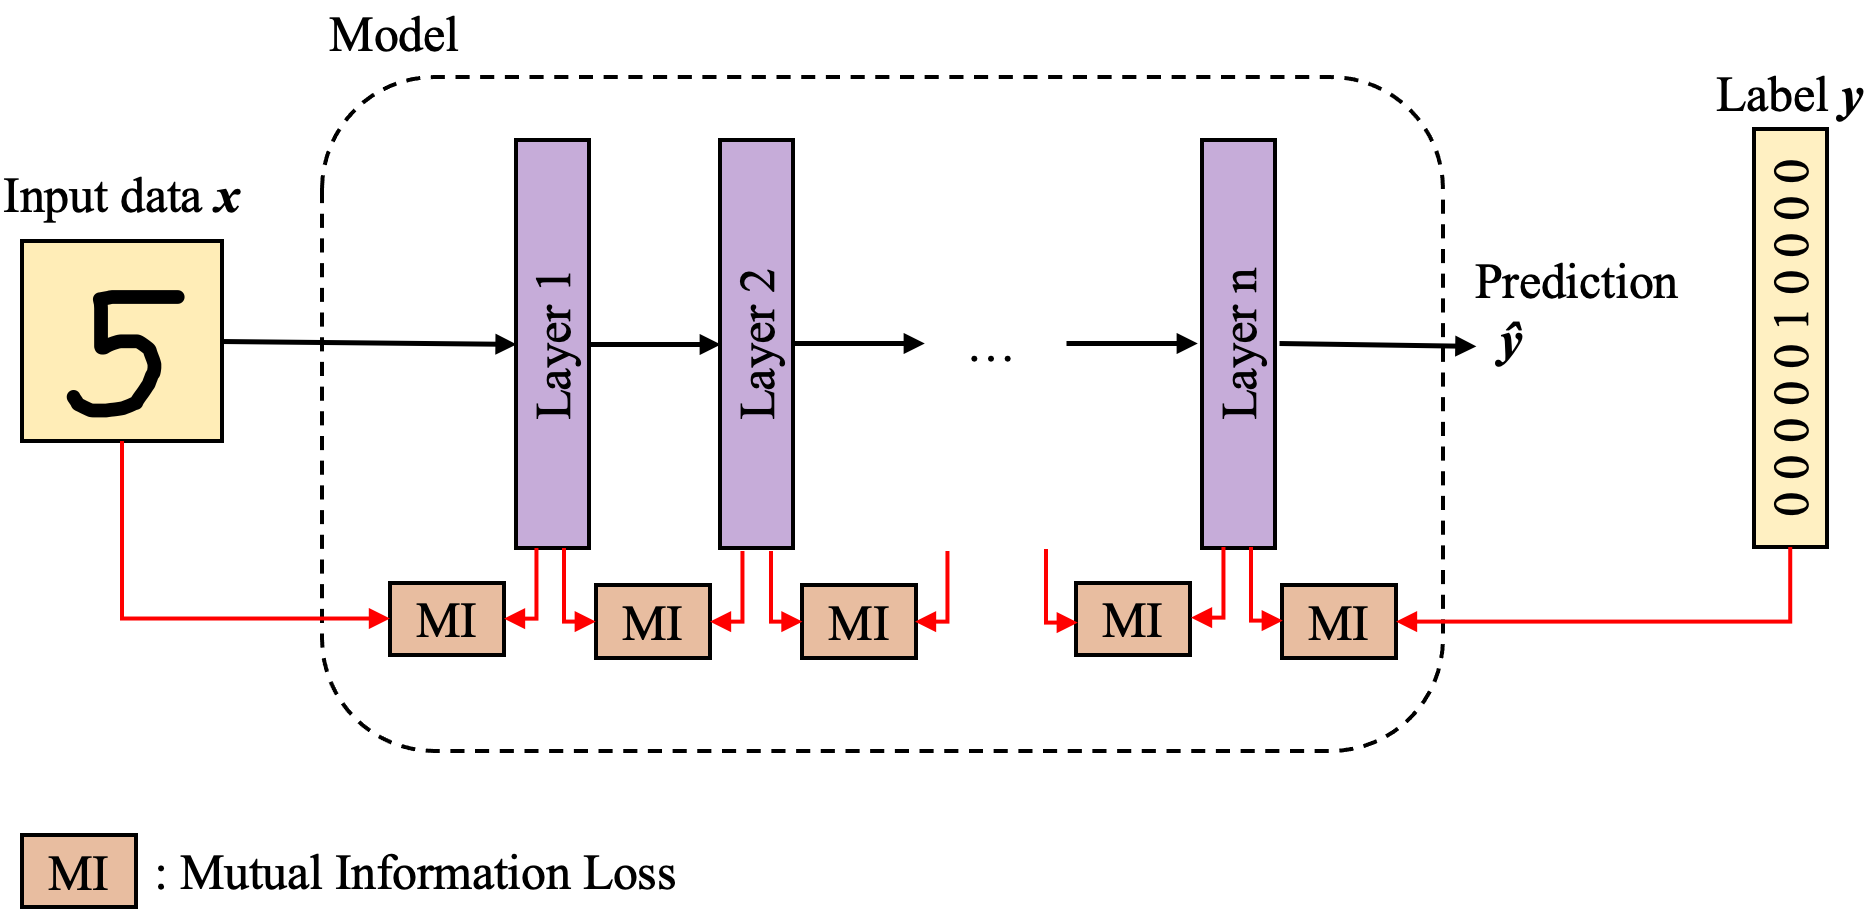
\includegraphics[width=0.99\textwidth]{mi_loss}
    \caption[Vertical self-organisation with mutual information loss]{Vertical self-organisation with mutual information loss: Each layer maximises the mutual information (MI) between its activations and the activations of the previous and subsequent layers. The first layer maximises the MI between its activations and the input image (instead of the previous layer), and the last layer maximises the MI between its activations and the image label (instead of the subsequent layer).}
    \figlbl{mi_loss}
\end{figure}

This process is visualised in Figure \figref{mi_loss}. 


TODO: Currently, various experiments are ongoing to find out how this can be implemented (therefore, yet to be explained in more detail).


%\subsection{Efficient Parallel Training}
%Idee: Nachfolgelayer einbeziehen in Loss -> Nachfolgelayer ist gefroren, Output muss aber möglichst gut sein (sollte Performance nicht verschlechtern von Nachfolgelayer) + eigene Performance verbessern


\section{Results}\seclbl{vertical_self_org_methods_results}
The results obtained by this model are presented below. It is important to note that these models aim not to achieve the best possible results in terms of classification accuracy on a benchmark. In large-scale comparisons, it has often been found that end-to-end backpropagation of error is far superior to other methods, especially in image classification \sidecite{Bartunov_Santoro_Richards_Marris_Hinton_Lillicrap_2018}. Instead, the aim here is to examine interesting concepts that are more biologically plausible and can inspire future work.

\subsection{Data set}\seclbl{vertical_self_org_methods_dataset}
The model was trained and evaluated on the MNIST \cite{Lecun_Bottou_Bengio_Haffner_1998} data set. It is a data set of handwritten digits with $60'000$ training samples and $10'000$ test samples.
In this thesis, the predefined training and test split is used.
The samples are images of a digit with the resolution $28 \times 28$ pixel in grayscale, i.e. has one colour channel.

In addition, the models are evaluated on MNIST-C \sidecite{Mu_Gilmer_2019}, a corrupted MNIST benchmark for testing the out-of-distribution robustness of image classification models. This data set consists of the MNIST data with $15$ types of corruptions applied to the samples.

\subsection{Baseline Model}
The base model consists of $4$ fully connected layers with $512$, $256$, $128$ and $64$ neurons as shown in \figref{vertical_org_arch1}.
No lateral connections or communication across multiple time steps are used for the baseline. In addition, the measures described in \secref{vertical_self_org_hierarchical_features} are not used.
This model achieves an accuracy on MNIST of $93.7\%$. This accuracy is remarkably good considering that the model has never been explicitly trained for classification with, for example, a cross-entropy loss.
Furthermore, the model is trained extremely fast because these local updates are suitable for batch-gradient descent and not only mini-batch gradient descent.
Each layer also has a different accuracy, typically in the range of $90.1\% - 92.9\%$. However, due to the implicit voting using the sum over the cosine similarities, the prediction of the entire model is better than that of a single layer.


\subsection{Lateral Connections}
TODO: How do lateral connections improve the result?


\subsection{Hierarchical Features}
TODO: How do hierarchical features improve the result?








%TODO: vereinheitliche Mathe: Was ist underline, was ist hochgestellt in Klammern ($z^{(i)}$) und was ist hochgestellt in eckigen Klammern? Bei NN: Was ist n, was ist m, ... (+ Lernraten Symbol, Loss Symbol, etc.)
%Sind alle Vektoren bold?

% TODO: target function und objective function vereinheitlichen
% TODO: net-fragment or net fragment



\setchapterpreamble[u]{\margintoc}
\chapter{Horizontal Self-Organisation}\chlbl{horizontal_self_org}
%% horizontal_self_org.tex
This chapter presents a method based on horizontal self-organisation (c.f. \secref{neuro_concepts_self_org}).
The idea of horizontal self-organisation is that the input is analysed by several smaller models instead of one big model.
This means that each network sees only a patch of the input data and cannot decide on its own what is represented in the input image but must agree on a representation with neighbouring models.
It is essential that each model is independent of the other models and that the parameters are not shared between them. Otherwise, the architecture would be comparable to vision transformer \sidecite{Dosovitskiy_Beyer_Kolesnikov_Weissenborn_Zhai_Unterthiner_Dehghani_Minderer_Heigold_Gelly_2021} and the input patches would no longer be analysed independently. Thus, the model would not be self-organising anymore. In the following, the methodology (i.e. how horizontal self-organisation is implemented) is presented, and the obtained results are discussed in detail.

\section{Methods}\seclbl{horizontal_self_org_methods}
A crucial design decision for horizontal self-organisation is the architecture of the models.
In this thesis are variational autoencoders \sidecite{Kingma_Welling_2014} (c.f. \secref{visual_rep_learning}) used to process patches of the input image as they have a continuous latent space and are thus more robust and better interpretable (c.f. \secref{neuro_concepts_net_fragments}).

Typical autoencoders fed an input image $\boldsymbol{x}$ through an encoder to map the input data to a latent space and through a decoder to recreate the image $\boldsymbol{\hat{x}}$. Thereby, the latent space is limited in size, forcing the model to compress the image with the encoder and to de-compress the image using the decoder (c.f. \secref{visual_rep_learning_ae}).

A variational autoencoder models the latent space as a multivariate Gaussian distribution. The input image $\boldsymbol{x}$ is also fed through an encoder, and a latent representation $\boldsymbol{h}$ is obtained. Afterwards, $\boldsymbol{h}$ is fed through two independent parallel fully connected layers to obtain the $\boldsymbol{\mu}$ and $\boldsymbol{\sigma}$ vectors of the multivariate Gaussian distribution. Afterwards, the re-parametrisation trick is used to sample a variable $\boldsymbol{z}'$ from this distribution:

\begin{equation}\eqlbl{hso_1}
	\boldsymbol{z}' \sim \mathcal{N}(\boldsymbol{\mu},\,\boldsymbol{\sigma}^{2} \cdot \epsilon)
\end{equation}

$\epsilon$ is a random variable sampled from  $\mathcal{N}(0, 1)$ and determines the magnitude of the variance. The sampled latent representation is then fed through the decoder, and the image $\hat{\boldsymbol{x}}$ is recreated. The model is trained to minimise a distance measure between the input image $\boldsymbol{x}$ and the reconstructed image $\hat{\boldsymbol{x}}$. In this thesis, the mean square error is used. For $m$ images $\boldsymbol{X} = \boldsymbol{x}^{(1)}, ..., \boldsymbol{x}^{(m)}$, the loss is defined as

\begin{equation}\eqlbl{hso_2}
	\mathcal{L}_{\text{rec}} = \frac{1}{m} \sum_{i=1}^{m} (\boldsymbol{x}^{(i)} - \boldsymbol{\hat{x}}^{(i)})^2
\end{equation}

However, the latent space does not form a multivariate Gaussian distribution based on this reconstruction loss and the network architecture. A second loss constraint is necessary to obtain a probability distribution in the latent space: Let $P(\boldsymbol{X})$ be the probability distribution of the data $\boldsymbol{X}$, $P(\boldsymbol{h})$ the probability distribution of the latent variable $\boldsymbol{h}$ and $P(\boldsymbol{X}|\boldsymbol{h})$ the conditional probability of generating $\boldsymbol{X}$ for a given $\boldsymbol{h}$. The objective of the encoder is to infer $P(\boldsymbol{h})$ from $P(\boldsymbol{h}|\boldsymbol{X})$ which is the probability distribution that maps $\boldsymbol{X}$ into latent space. Simply put: the goal is to know the latent variable $\boldsymbol{h}$ of the input data $\boldsymbol{X}$.
However, $P(\boldsymbol{h}|\boldsymbol{X})$ is unknown and we have to estimate it from a simpler distribution $Q(\boldsymbol{h}|\boldsymbol{X})$. This simpler distribution $Q(\boldsymbol{h}|\boldsymbol{X})$ is learned by the encoder and should be as close as possible to the real distribution $P(\boldsymbol{h}|\boldsymbol{X})$. This is accomplished by minimising the KL divergence\sidenote{the Kullback-Leibler (KL) divergence can ``measure'' the difference between two probability distributions} between these two probability distributions.

\begin{equation}\eqlbl{hso_3}
	KL \left[ Q(\boldsymbol{h}|\boldsymbol{X}) || P(\boldsymbol{h}|\boldsymbol{X}) \right] = E \left[ \log Q(\boldsymbol{h}|\boldsymbol{X}) - \log P(\boldsymbol{h}|\boldsymbol{X}) \right]
\end{equation}

In the case of two Gaussian distributions, the KL divergence is defined as:
\begin{equation}\eqlbl{hso_4}
	KL\left[ \mathcal{N}_Q(\boldsymbol{\mu}_Q, \boldsymbol{\sigma}_Q)||\mathcal{N}_P(\boldsymbol{\mu}_P, \boldsymbol{\sigma}_P) \right] = \log \frac{\boldsymbol{\sigma}_P}{\boldsymbol{\sigma}_Q} + \frac{\boldsymbol{\sigma}_Q^2 + (\boldsymbol{\mu}_Q-\boldsymbol{\mu}_P)^2}{2\boldsymbol{\sigma}_P^2} - \frac{1}{2}
\end{equation}


If the target distribution $P(\boldsymbol{h}|\boldsymbol{X})$ is a multivariate Gaussian distribution with $\boldsymbol{\mu}_P = 0$ and $\boldsymbol{\sigma}_P=1$ (i.e. $\mathcal{N}(0, 1)$) and the encoder predicts $\boldsymbol{\mu}_Q$ and $\boldsymbol{\sigma}_Q$ to model $Q(\boldsymbol{h}|\boldsymbol{X})$ as $\mathcal{N}(\boldsymbol{\mu}_Q, \boldsymbol{\sigma}_Q)$, then the KL divergence simplifies to


\begin{equation*}\eqlbl{hso_5}
\begin{split}
		\mathcal{L}_{KLD} = KL \left[ \mathcal{N}_Q(\boldsymbol{\mu}_Q, \boldsymbol{\sigma}_Q)||\mathcal{N}(0, 1) \right] & = -\log \boldsymbol{\sigma}_Q + \frac{\boldsymbol{\sigma}_Q^2 \boldsymbol{\mu}_Q^2}{2} - \frac{1}{2} \\
		 & = \frac{1}{2} \left( \boldsymbol{\sigma}_Q^2 \boldsymbol{\mu}_Q^2 - 1 - 2\log \boldsymbol{\sigma}_Q \right)
\end{split}
\end{equation*}

Interested readers may find a formal proof of the formulas above and a more detailed derivation in the original paper \cite{Kingma_Welling_2014}.
Thus, the loss for the variational autoencoder is defined as:


\begin{equation*}\eqlbl{hso_6}
\begin{split}
		\mathcal{L}_{\text{VAE}} & = \mathcal{L}_{\text{rec}} + \beta \cdot KL \left[ \mathcal{N}_Q(\boldsymbol{\mu}_Q, \boldsymbol{\sigma}_Q)||\mathcal{N}(0, 1) \right] \\
		  & = \underbrace{\frac{1}{n} \sum_{i=1}^{n} (\boldsymbol{x}_i - \boldsymbol{\hat{x}}_i)^2}_{\text{reconstruction loss}} + \lambda \cdot \overbrace{\frac{1}{2} (\boldsymbol{\sigma}_Q^2 \boldsymbol{\mu}_Q^2 - 1 - 2\log \boldsymbol{\sigma}_Q)}^{\text{KL divergence}}
\end{split}
\end{equation*}

where $\beta$ is a weight factor of the KL divergence. Training a variational autoencoder with this loss function can lead to excellent image reconstruction.
In the case of horizontal self-organisation, however, a well-formed latent space is of more interest than an outstanding image reconstruction: The goal is to obtain good image representations, and thus the goal is to have a well-formed latent space and not perfect reconstruction.
Variational autoencoders have the notorious problem that the KL divergence term becomes vanishingly small during training \sidecite{bowman2016generating}. This issue is known as the KL vanishing problem.
This problem can be alleviated by applying annealing schedules to the KL term (i.e., changing $\beta$ over time).
In this thesis, monotonic annealing is used as proposed by \sideciteay{bowman2016generating}.
However, for a slight increase in computational costs, cyclic annealing strategies might lead to even better results \sidecite{Fu_Li_Liu_Gao_Celikyilmaz_Carin_2019}.
The disadvantage is that training with cyclic annealing takes longer, which outweighs the advantage of only minimally better latent representation.
These annealing strategies are shown in Figure \figref{beta_annealing}. When $\beta$ is small, the model is forced to focus on reconstructing the input rather than minimising the KL loss.
When $\beta$ is increased, the model gradually improves the shape of the data distribution in the latent space.

\begin{figure}[h]
    \centering
    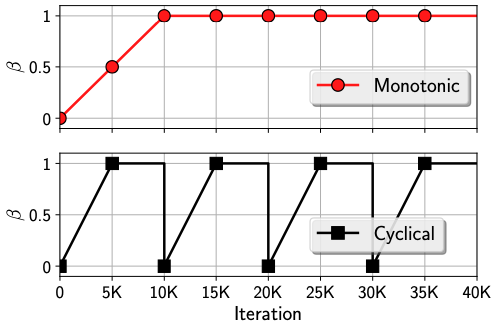
\includegraphics[width=0.5\textwidth]{beta_annealing}
    \caption[Annealing strategy of the KL weight term in variational autoencoders]{Two annealing strategies for the $\beta$ term that weights the KL divergence in the loss function of variational autoencoders. The upper graph shows a monotonic increase of $\beta$, and the lower graph a cyclical annealing strategy. The picture is from \cite{Fu_Li_Liu_Gao_Celikyilmaz_Carin_2019}.}
    \figlbl{beta_annealing}
\end{figure}

In this thesis, $4$ variational autoencoders are used. Each VAE consists of an encoder, two fully-connected layers to calculate $\boldsymbol{\mu}$ and $\boldsymbol{\sigma}$, and a decoder.
The encoder consists of $3$  convolutional layers with $32$, $64$, and $128$ channels. Each convolutional layer has a stride of $2$, halving the input size in each layer.
The decoder has the inverse structure of the encoder, i.e. $3$ transposed convolutional layers with $128$, $64$, and $32$ channels.
The fully connected layer for predicting $\boldsymbol{\mu}$ and $\boldsymbol{\sigma}$ have $32$ neurons.
The network architecture is shown in \figref{horizontal_org_arch1}.

\begin{figure}[h]
    \centering
    \resizebox{0.99\textwidth}{!}
{
\begin{tikzpicture}
\tikzstyle{connection}=[ultra thick,every node/.style={sloped,allow upside down},draw=\edgecolor,opacity=0.7]
\tikzstyle{copyconnection}=[ultra thick,every node/.style={sloped,allow upside down},draw={rgb:blue,4;red,1;green,1;black,3},opacity=0.7]


\node[canvas is zy plane at x=0] (input) at (0,0,0) {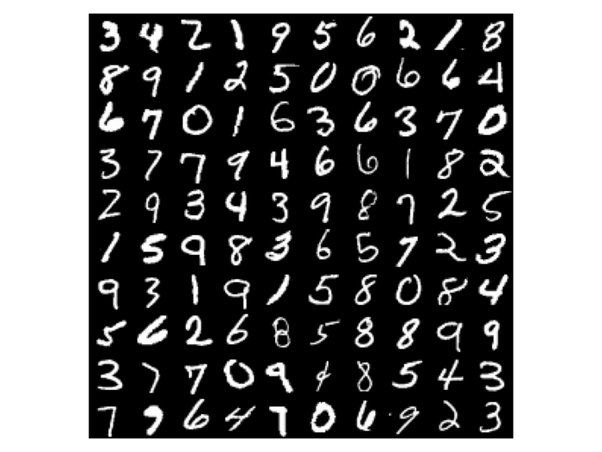
\includegraphics[width=8cm,height=8cm]{imgs/mnist.jpeg}};


\pic[shift={(3,0,0)}] at (input) 
    {Box={
        name=conv1,
        caption=Conv + ReLU,
        xlabel={{1, }},
        zlabel=32,
        fill=\ConvColor,
        height=20,
        width=2,
        depth=20
        }
    };


\draw [connection]  (input) ++(0,0,0)    -- node {\midarrow} (conv1-west);


\pic[shift={(2,0,0)}] at (conv1-east) 
    {Box={
        name=conv2,
        caption=Conv + ReLU,
        xlabel={{32, }},
        zlabel=64,
        fill=\ConvColor,
        height=12,
        width=4,
        depth=12
        }
    };


\draw [connection]  (conv1-east)    -- node {\midarrow} (conv2-west);


\pic[shift={(2,0,0)}] at (conv2-east) 
    {Box={
        name=conv3,
        caption=Conv + ReLU,
        xlabel={{64, }},
        zlabel=128,
        fill=\ConvColor,
        height=6,
        width=6,
        depth=6
        }
    };


\draw [connection]  (conv2-east)    -- node {\midarrow} (conv3-west);


\pic[shift={(2,2,0)}] at (conv3-east) 
    {Box={
        name=fcn1,
        caption=FC + ReLU,
        xlabel={{" ","dummy"}},
        zlabel=32,
        fill=\SoftmaxColor,
        opacity=0.8,
        height=3,
        width=3,
        depth=6
        }
    };


\pic[shift={(2,-2,0)}] at (conv3-east) 
    {Box={
        name=fcn2,
        caption=FC + ReLU,
        xlabel={{" ","dummy"}},
        zlabel=32,
        fill=\SoftmaxColor,
        opacity=0.8,
        height=3,
        width=3,
        depth=6
        }
    };


\draw [connection]  (conv3-east)    -- node {\midarrow} (fcn1-west);


\draw [connection]  (conv3-east)    -- node {\midarrow} (fcn2-west);


\pic[shift={(2,-2,0)}] at (fcn1-east) 
    {Box={
        name=conv4,
        caption=Conv + ReLU,
        xlabel={{128, }},
        zlabel=64,
        fill=\ConvColor,
        height=6,
        width=6,
        depth=6
        }
    };


\draw [connection]  (fcn1-east)    -- node {\midarrow} (conv4-west);


\draw [connection]  (fcn2-east)    -- node {\midarrow} (conv4-west);


\pic[shift={(2,0,0)}] at (conv4-east) 
    {Box={
        name=conv5,
        caption=Conv + ReLU,
        xlabel={{64, }},
        zlabel=32,
        fill=\ConvColor,
        height=12,
        width=4,
        depth=12
        }
    };


\draw [connection]  (conv4-east)    -- node {\midarrow} (conv5-west);


\pic[shift={(2,0,0)}] at (conv5-east) 
    {Box={
        name=conv6,
        caption=Conv + ReLU,
        xlabel={{32, }},
        zlabel=1,
        fill=\ConvColor,
        height=20,
        width=2,
        depth=20
        }
    };


\draw [connection]  (conv5-east)    -- node {\midarrow} (conv6-west);


\node[canvas is zy plane at x=3] (output) at (conv6-east) {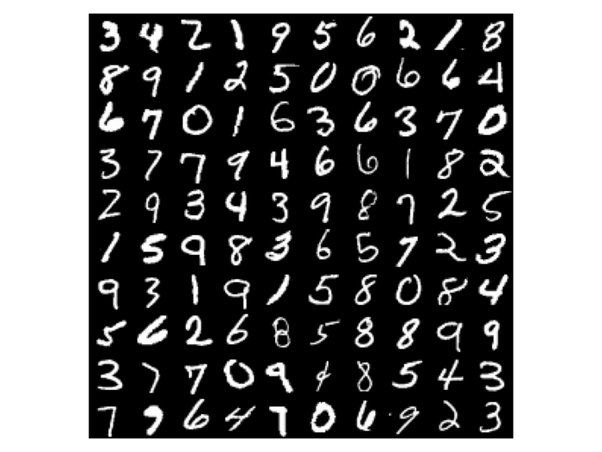
\includegraphics[width=8cm,height=8cm]{imgs/mnist.jpeg}};


\draw [connection]  (conv6-east)     -- node {\midarrow} ($(output) + (0.5,0,0)$);


\end{tikzpicture}
}
    \caption[Architecture of the variational autoencoder used for horizontal self-organisation]{Architecture of the variational autoencoder used for horizontal self-organisation.}
    \figlbl{horizontal_org_arch1}
\end{figure}

Each VAE is trained independently to minimise the loss function as described in \eqref{hso_6}.
Adam \sidecite{Kingma_Ba_2017} is used as an optimisation algorithm with a learning rate of $1\cdot 10^{-3}$, and the mini-batch size is $32$.


\subsection{Predicting bigger Patches}\seclbl{horizontal_self_org_methods_bigger_patches}
Applying monotonic annealing to the KL divergence weight term $\beta$ is the first measure to improve the latent space distribution.
Another measure is to predict bigger patches.
The VAEs have a very limited field of view and cannot distinguish some of the digits on their own (c.f. \secref{horizontal_self_org_methods_communication}).
However, by predicting bigger patches, the VAEs can be encouraged to distinguish similar-looking patches better.
For example, the patches for the digits $4$, $5$, and $6$ look very similar for the first VAE that receives the patch extracted from the top left corner of the samples (c.f. \figref{average_sample}).
Since the target prediction of these two digits is similar, they are located closely together in the latent space.
When a VAE predicts bigger patches or the entire image, the target predictions of the digits $4$, $5$, and $6$ become different. Thus, while similar latent representations are sufficient to predict only a patch of these digits, predicting larger patches or the whole picture requires more separated latent representations.
Thus, predicting bigger patches helps push apart latent representations of objects with a high patch-wise similarity but a low image-wise similarity.


In this thesis, an additional layer is used in the decoder to predict larger patches. In fact, the last layer with $32$ channels and a stride of $2$ is used twice so that the decoder has $4$ transposed convolutional layers with $128$, $64$, $32$, and $32$ channels. Thus, the output size of the decoder is doubled. This architecture is shown in Figure \figref{horizontal_org_arch2}.


\begin{figure}[h]
    \centering
    \resizebox{0.99\textwidth}{!}
{
\begin{tikzpicture}
\tikzstyle{connection}=[ultra thick,every node/.style={sloped,allow upside down},draw=\edgecolor,opacity=0.7]
\tikzstyle{copyconnection}=[ultra thick,every node/.style={sloped,allow upside down},draw={rgb:blue,4;red,1;green,1;black,3},opacity=0.7]


\node[canvas is zy plane at x=0] (input) at (0,0,0) {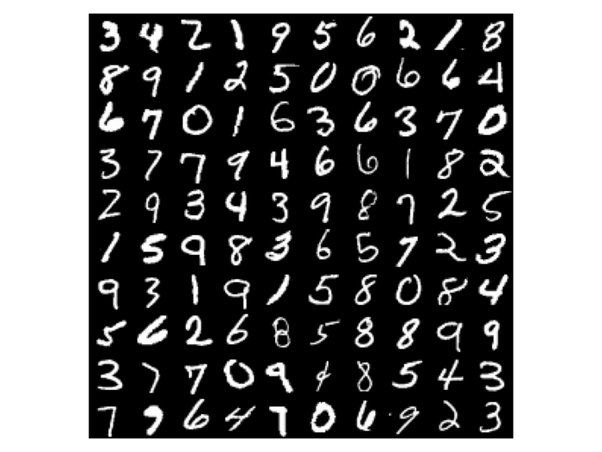
\includegraphics[width=8cm,height=8cm]{imgs/mnist.jpeg}};


\pic[shift={(3,0,0)}] at (input) 
    {Box={
        name=conv1,
        caption=Conv + ReLU,
        xlabel={{1, }},
        zlabel=32,
        fill=\ConvColor,
        height=20,
        width=2,
        depth=20
        }
    };


\draw [connection]  (input) ++(0,0,0)    -- node {\midarrow} (conv1-west);


\pic[shift={(2,0,0)}] at (conv1-east) 
    {Box={
        name=conv2,
        caption=Conv + ReLU,
        xlabel={{32, }},
        zlabel=64,
        fill=\ConvColor,
        height=12,
        width=4,
        depth=12
        }
    };


\draw [connection]  (conv1-east)    -- node {\midarrow} (conv2-west);


\pic[shift={(2,0,0)}] at (conv2-east) 
    {Box={
        name=conv3,
        caption=Conv + ReLU,
        xlabel={{64, }},
        zlabel=128,
        fill=\ConvColor,
        height=6,
        width=6,
        depth=6
        }
    };


\draw [connection]  (conv2-east)    -- node {\midarrow} (conv3-west);


\pic[shift={(2,2,0)}] at (conv3-east) 
    {Box={
        name=fcn1,
        caption=FC + ReLU,
        xlabel={{" ","dummy"}},
        zlabel=32,
        fill=\SoftmaxColor,
        opacity=0.8,
        height=3,
        width=3,
        depth=6
        }
    };


\pic[shift={(2,-2,0)}] at (conv3-east) 
    {Box={
        name=fcn2,
        caption=FC + ReLU,
        xlabel={{" ","dummy"}},
        zlabel=32,
        fill=\SoftmaxColor,
        opacity=0.8,
        height=3,
        width=3,
        depth=6
        }
    };


\draw [connection]  (conv3-east)    -- node {\midarrow} (fcn1-west);


\draw [connection]  (conv3-east)    -- node {\midarrow} (fcn2-west);


\pic[shift={(2,-2,0)}] at (fcn1-east) 
    {Box={
        name=conv4,
        caption=Conv + ReLU,
        xlabel={{128, }},
        zlabel=64,
        fill=\ConvColor,
        height=6,
        width=6,
        depth=6
        }
    };


\draw [connection]  (fcn1-east)    -- node {\midarrow} (conv4-west);


\draw [connection]  (fcn2-east)    -- node {\midarrow} (conv4-west);


\pic[shift={(2,0,0)}] at (conv4-east) 
    {Box={
        name=conv5,
        caption=Conv + ReLU,
        xlabel={{64, }},
        zlabel=32,
        fill=\ConvColor,
        height=12,
        width=4,
        depth=12
        }
    };


\draw [connection]  (conv4-east)    -- node {\midarrow} (conv5-west);


\pic[shift={(2,0,0)}] at (conv5-east) 
    {Box={
        name=conv6,
        caption=Conv + ReLU,
        xlabel={{32, }},
        zlabel=32,
        fill=\ConvColor,
        height=20,
        width=2,
        depth=20
        }
    };


\draw [connection]  (conv5-east)    -- node {\midarrow} (conv6-west);


\pic[shift={(2,0,0)}] at (conv6-east) 
    {Box={
        name=conv7,
        caption=Conv + ReLU,
        xlabel={{32, }},
        zlabel=1,
        fill=\ConvColor,
        height=20,
        width=2,
        depth=20
        }
    };


\draw [connection]  (conv6-east)    -- node {\midarrow} (conv7-west);


\node[canvas is zy plane at x=3] (output) at (conv7-east) {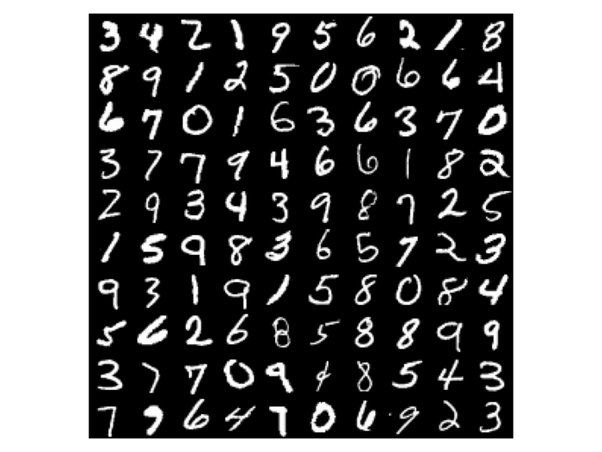
\includegraphics[width=8cm,height=8cm]{imgs/mnist.jpeg}};


\draw [connection]  (conv6-east)     -- node {\midarrow} ($(output) + (0.5,0,0)$);


\end{tikzpicture}
}
    \caption[Architecture of the VAE used for horizontal self-organisation with bigger field-of-view up-sampling]{Architecture of the variational autoencoder used for horizontal self-organisation with bigger field-of-view up-sampling.}
    \figlbl{horizontal_org_arch2}
\end{figure}

When using $4$ VAEs, the input is divided into $4$ patches. If the decoder makes the output twice as large as the input by up-sampling,  the entire image is predicted by each of the VAEs. This process is visualised in \figref{bigger_patches}.

\begin{figure}[h]
    \centering
    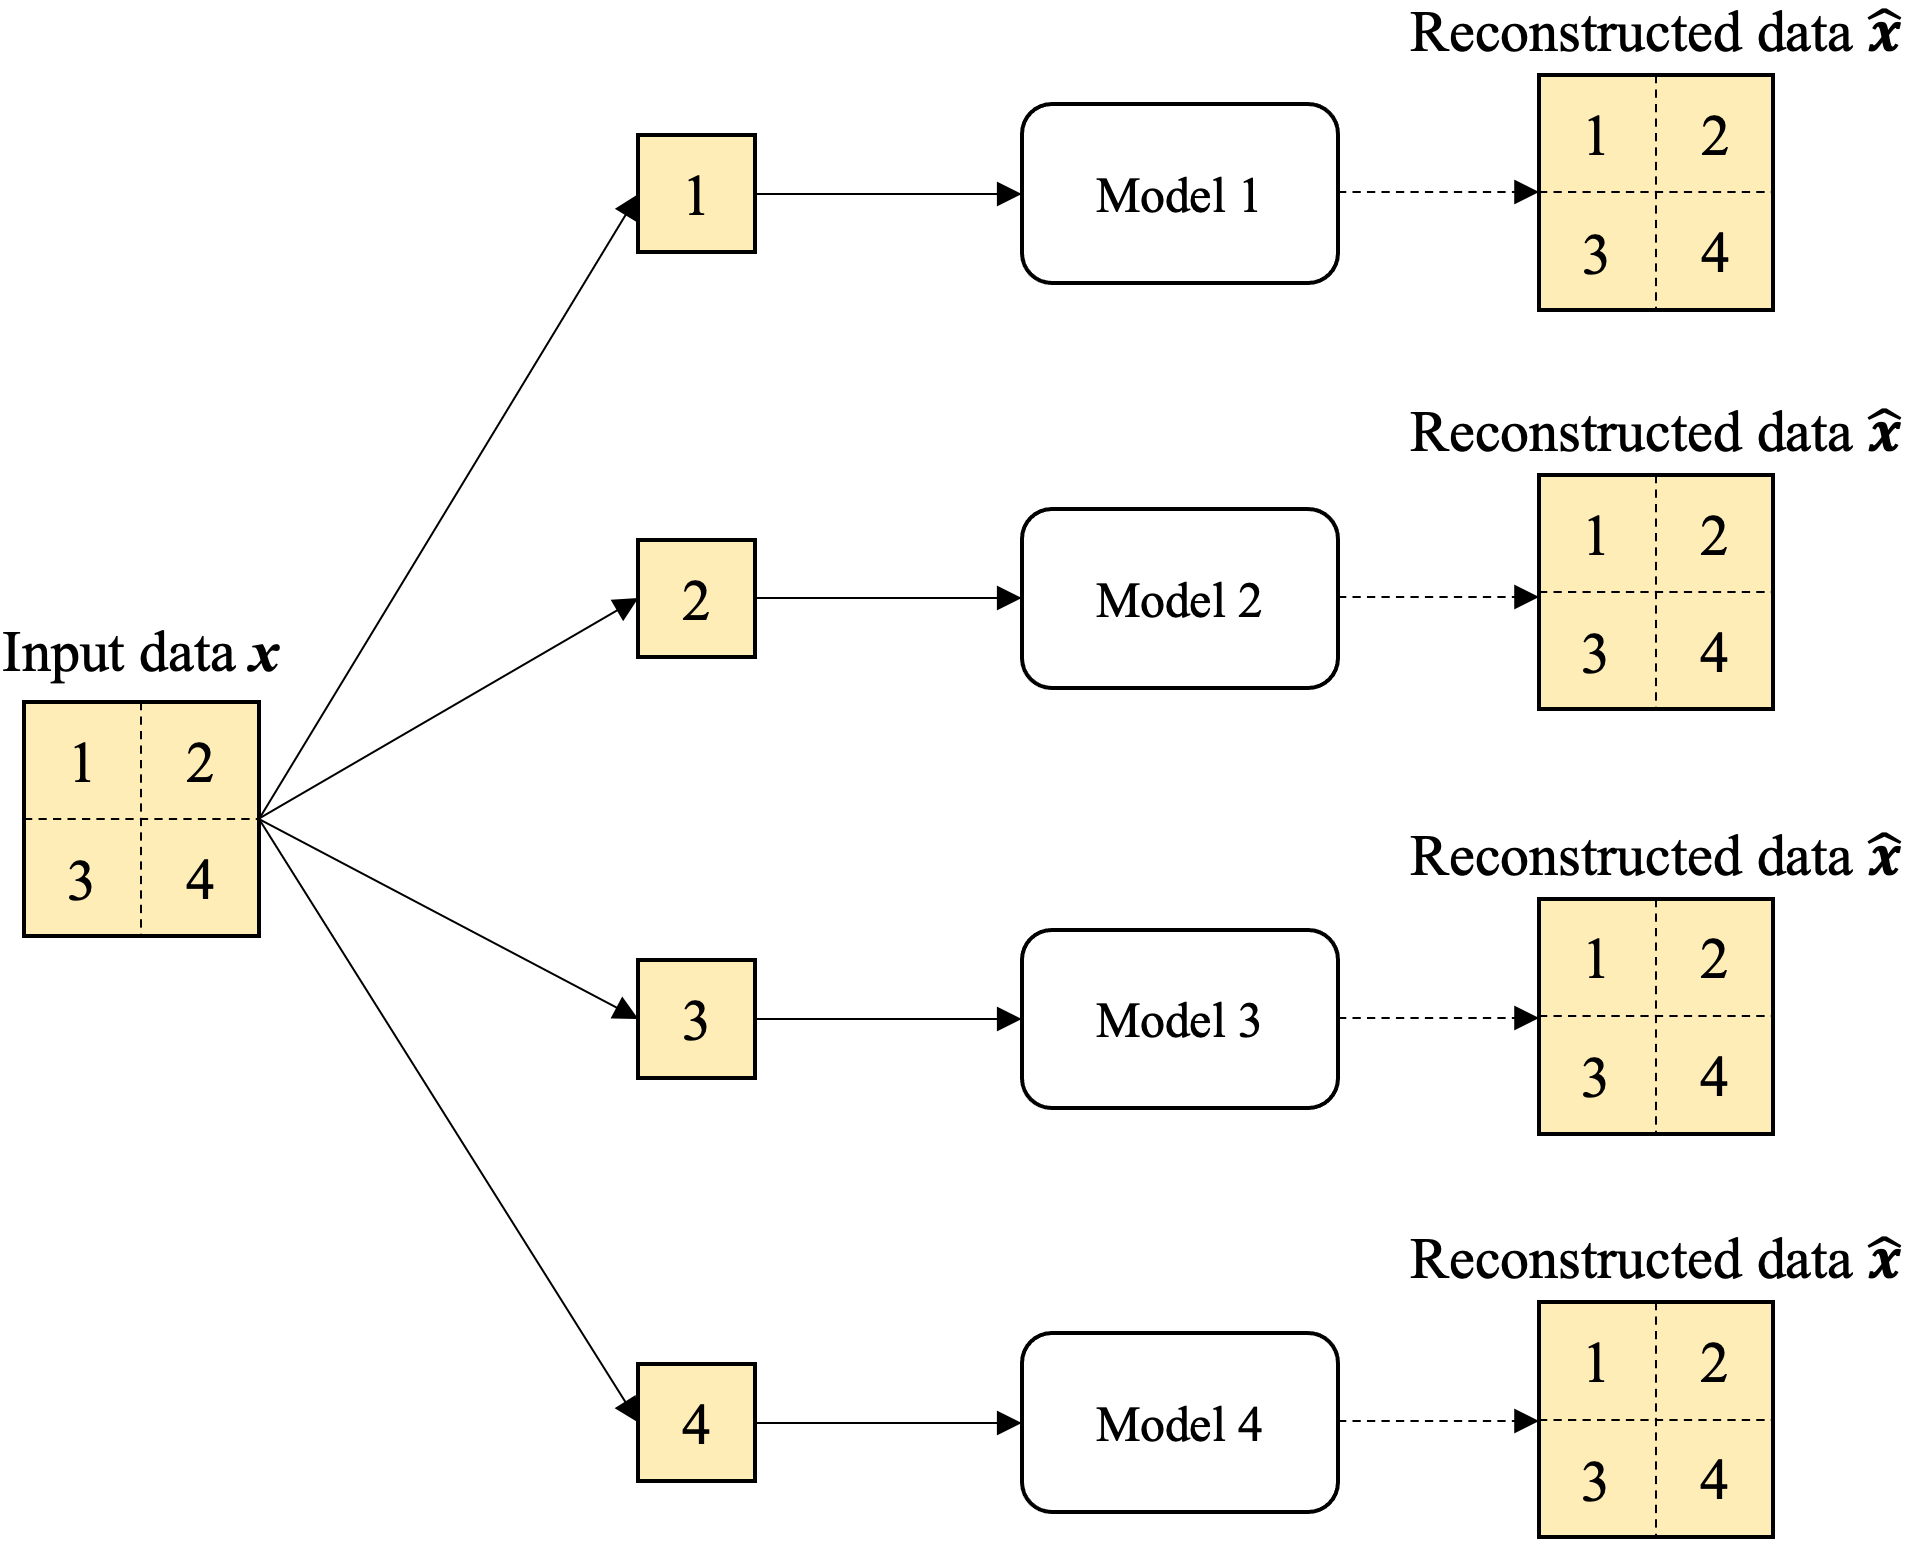
\includegraphics[width=0.99\textwidth]{bigger_patches}
    \caption[Reconstruction of bigger output than input patches]{Four models receive a quarter of the image as input patch to predict the entire image.}
    \figlbl{bigger_patches}
\end{figure}



\subsection{Communication}\seclbl{horizontal_self_org_methods_communication}
The VAEs receive patches of the input image and thus have a limited field of view on the image.
Figure \figref{average_sample} visualises the patches that are fed into the VAEs when the MNIST data set \cite{Lecun_Bottou_Bengio_Haffner_1998} is used.
The first row shows the average of all images of the same class. Thus, these images are very representative for the data set.
However, none of the models receives the entire image as input. Instead, the patches shown in the 2nd to the 5th row are fed into the VAEs.
The patches, which only depict a quarter of the image, look rather similar for some classes. For example, the top-left patches of the classes $0$ and $9$, as well as the classes $4$, $5$, and $6$, look very similar.
Thus, these classes are not separable by \emph{one} single VAE on its own.
Therefore, communication with neighbouring models is necessary to agree on an image representation.

\begin{figure}[h]
    \centering
    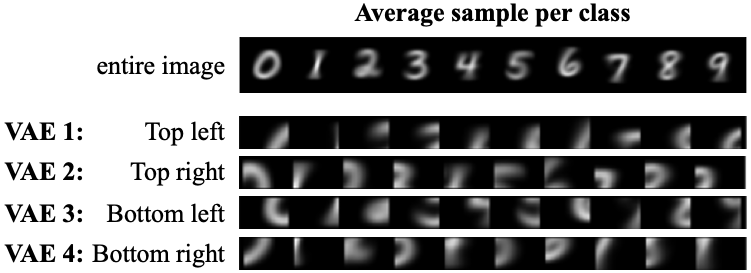
\includegraphics[width=0.99\textwidth]{average_sample}
    caption[Average sample of the MNIST data set per class]{The average of all samples in the MNIST data set for each class. The first row shows the average of all samples, and the 2nd to 5th row is the average per patch fed into the models.}
    \figlbl{average_sample}
\end{figure}


This concept links well to the biological model: A single VAE can be seen as a neuron or a group of neurons. Initially, the VAEs have many suggestions to which classes the received patch could belong. However, through communication with neighbouring VAEs, suggestions are constantly ruled out because neighbouring VAEs do not support them. Thus, out of many suggestions, only the most valid ones are retained, resulting in an image representation. The biological model behaves similarly: At first, many neurons are active because they are excited by the captured image. However, this strong activation quickly becomes sparse as only the neurons supporting each other remain active. This process leads to the emergence of higher-level features (i.e. net fragments) that are representative of the captured input \sidecite{Malsburg_1987}.

One of the biggest strengths of autoencoders is that they do not rely on labels but can be trained in an unsupervised manner. To keep this strength, also communication should not rely on labels. Therefore, different types of communication are proposed that work without labels: communication based on latent representations, communication based on reconstructed images, and communication via a dedicated communication channel.

All these types of communication take place over two or more time steps. First, image patches are reconstructed by all VAEs. As a result, each VAE generates information in latent space. Then, this information can be communicated to the neighbouring VAEs. Thus, in a second time-step, the VAEs have more information available: their prediction is based on the reconstructed image patch and information from neighbouring VAEs. This additional information allows them to improve their prediction. The process can be repeated over a fixed number of time steps or until the network reaches an attractor state (i.e. the latent representations no longer change). In the following, different types of communication are proposed.


\subsubsection{Model Heads}
Each VAE learns the mapping from a patch to a latent space with Gaussian distribution, i.e. obtains a $\boldsymbol{mu}$ and $\boldsymbol{sigma}$ for each sample that is used to predict a reconstructed version of the input.
The arrangement of the representations within the latent space is not predetermined by an external system but is fself-organised. A consequence of independent systems is that $\boldsymbol{mu}$ and $\boldsymbol{sigma}$ have different meanings in the latent spaces of different VAEs. Thus, one VAE cannot interpret the Gaussian parameters of another VAE.

In this thesis, it is proposed to learn a linear transformation to map the Gaussian parameters of one VAE to the Gaussian parameters of another VAE. The mapping from $\boldsymbol{mu}_1$ to $\boldsymbol{mu}_2$, respectively from $\boldsymbol{sigma}_1$ to $\boldsymbol{sigma}_2$ is done by the simple transformation

\begin{equation}\eqlbl{hso_7}
	\boldsymbol{\hat{\mu}}_2 = \boldsymbol{w}_{m12} \cdot \boldsymbol{\mu}_1
\end{equation}

resp.

\begin{equation}\eqlbl{hso_8}
	\boldsymbol{\hat{\sigma}}_2 = \boldsymbol{w}_{s12} \cdot \boldsymbol{\sigma}_1
\end{equation}

The weights $\boldsymbol{w}_{mij}$ and $\boldsymbol{w}_{sij}$ between VAE $i$ and VAE $j$ are learned by minimising the mean square error with gradient descent between the predicted and true Gaussian parameters, i.e. between $\boldsymbol{\mu}_j$ and $\boldsymbol{\hat{\mu}}_j$, resp. $\boldsymbol{\sigma}_j$ and $\boldsymbol{\hat{\sigma}}_j$. This process is illustrated for VAE 1 in \figref{hso_head}: First, the Gaussian parameters of each model must be predicted for the same sample. Afterwards, the Gaussian parameters of one model can be used to predict the Gaussian parameters of the other models with a linear transformation.

\begin{figure}[h]
    \centering
    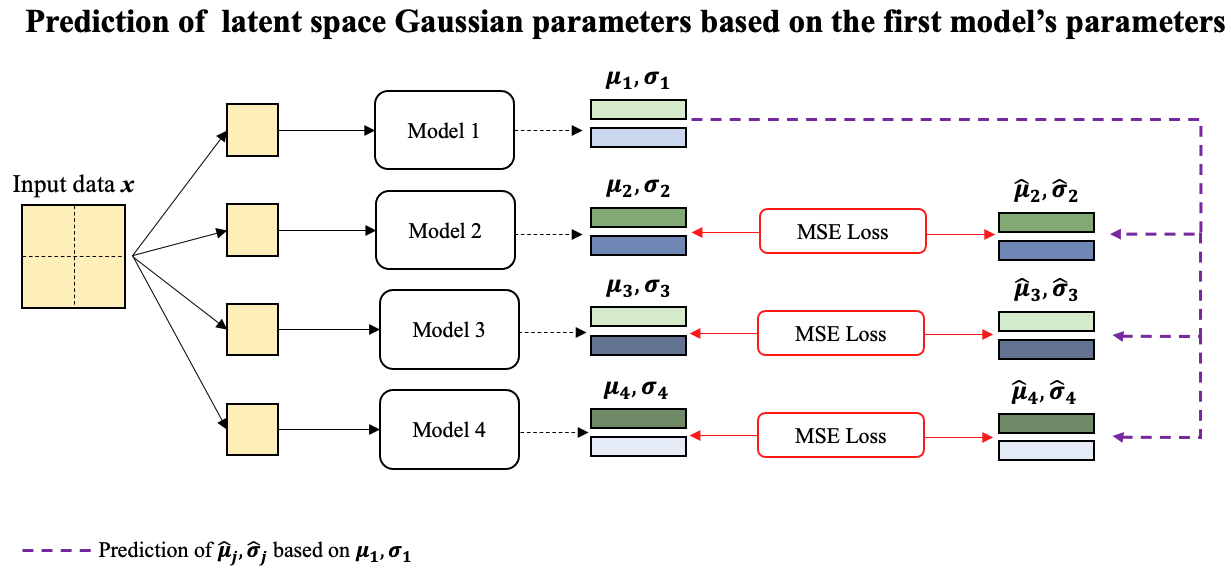
\includegraphics[width=0.99\textwidth]{hso_head}
    \caption[Prediction of Gaussian parameters of other VAEs]{Visualisation of how the first VAE can predict the Gaussian parameters of the other VAEs.}
    \figlbl{hso_head}
\end{figure}

If each VAE predicts the Gaussian parameters of the other VAEs, then these predictions can be communicated, and each VAE receives further suggestions from neighbouring VAEs. Thus, each VAE has its own calculated Gaussian parameters and suggestions from neighbours about what its Gaussian parameters might be. This allows a VAE to correct its prediction. Each VAE receives additional information because the suggestions made by neighbouring VAEs are based on a different patch. For example, the VAE that sees only one patch from the top left of the image cannot distinguish the digits $5$ and $6$. On the other hand, the VAE that sees the patch at the bottom left can distinguish these digits. Thus, the VAE at the bottom left can help the VAE at the top left to choose a better latent representation.

TODO: At the moment, various experiments are still ongoing to find out how this can be implemented (therefore, not yet explained in more detail).




















\subsubsection{Reconstructed Images}
As described in \secref{horizontal_self_org_methods_bigger_patches}, the prediction of larger patches helps to better arrange the latent space. The prediction of larger patches can also be used for communication with neighbouring VAEs. Instead of extracting representations from the latent space and transmitting them to neighbouring VAEs as described in the last section, the reconstructed image can also be exchanged. This is done by predicting a part of the image in a first time-step and by adding this prediction to an additional input channel of another VAE in the next time-step. Various data can be forwarded to other VAEs:% and is explained below. Let $\boldymbol{x}$ be the input image and $\boldymbol{\hat{x}}$ the reconstructed image. For $n$ VAEs, the input sample $\boldymbol{x}$ is split into $n$ non-overlapping patches $\boldymbol{x}^{(1)}, ..., \boldymbol{x}^{(n)}$. The reconstructed patches are denoted as $\boldymbol{\hat{x}}^{(1)}, ..., \boldymbol{\hat{x}}^{(n)}$. If a VAE reconstructs the same patch as it received as input, $\boldymbol{x}^{(i)} \approx \boldymbol{\hat{x}}^{(i)}$ is valid. However, when a bigger patch is predicted than the one that was fed into the model, then this term is not valid anymore, i.e. $\boldymbol{x}^{(i)} \not\approx \boldymbol{\hat{x}}^{(i)}$. However, if only a part of the prediction $\boldymbol{\hat{x}}^{(i)}$ is considered (i.e. the prediction is cropped), then $\boldymbol{x}^{(i)}$ is contained in this cropped version of the prediction $\boldymbol{\hat{x}}^{(i)}_C$.


\begin{figure}
    \centering
    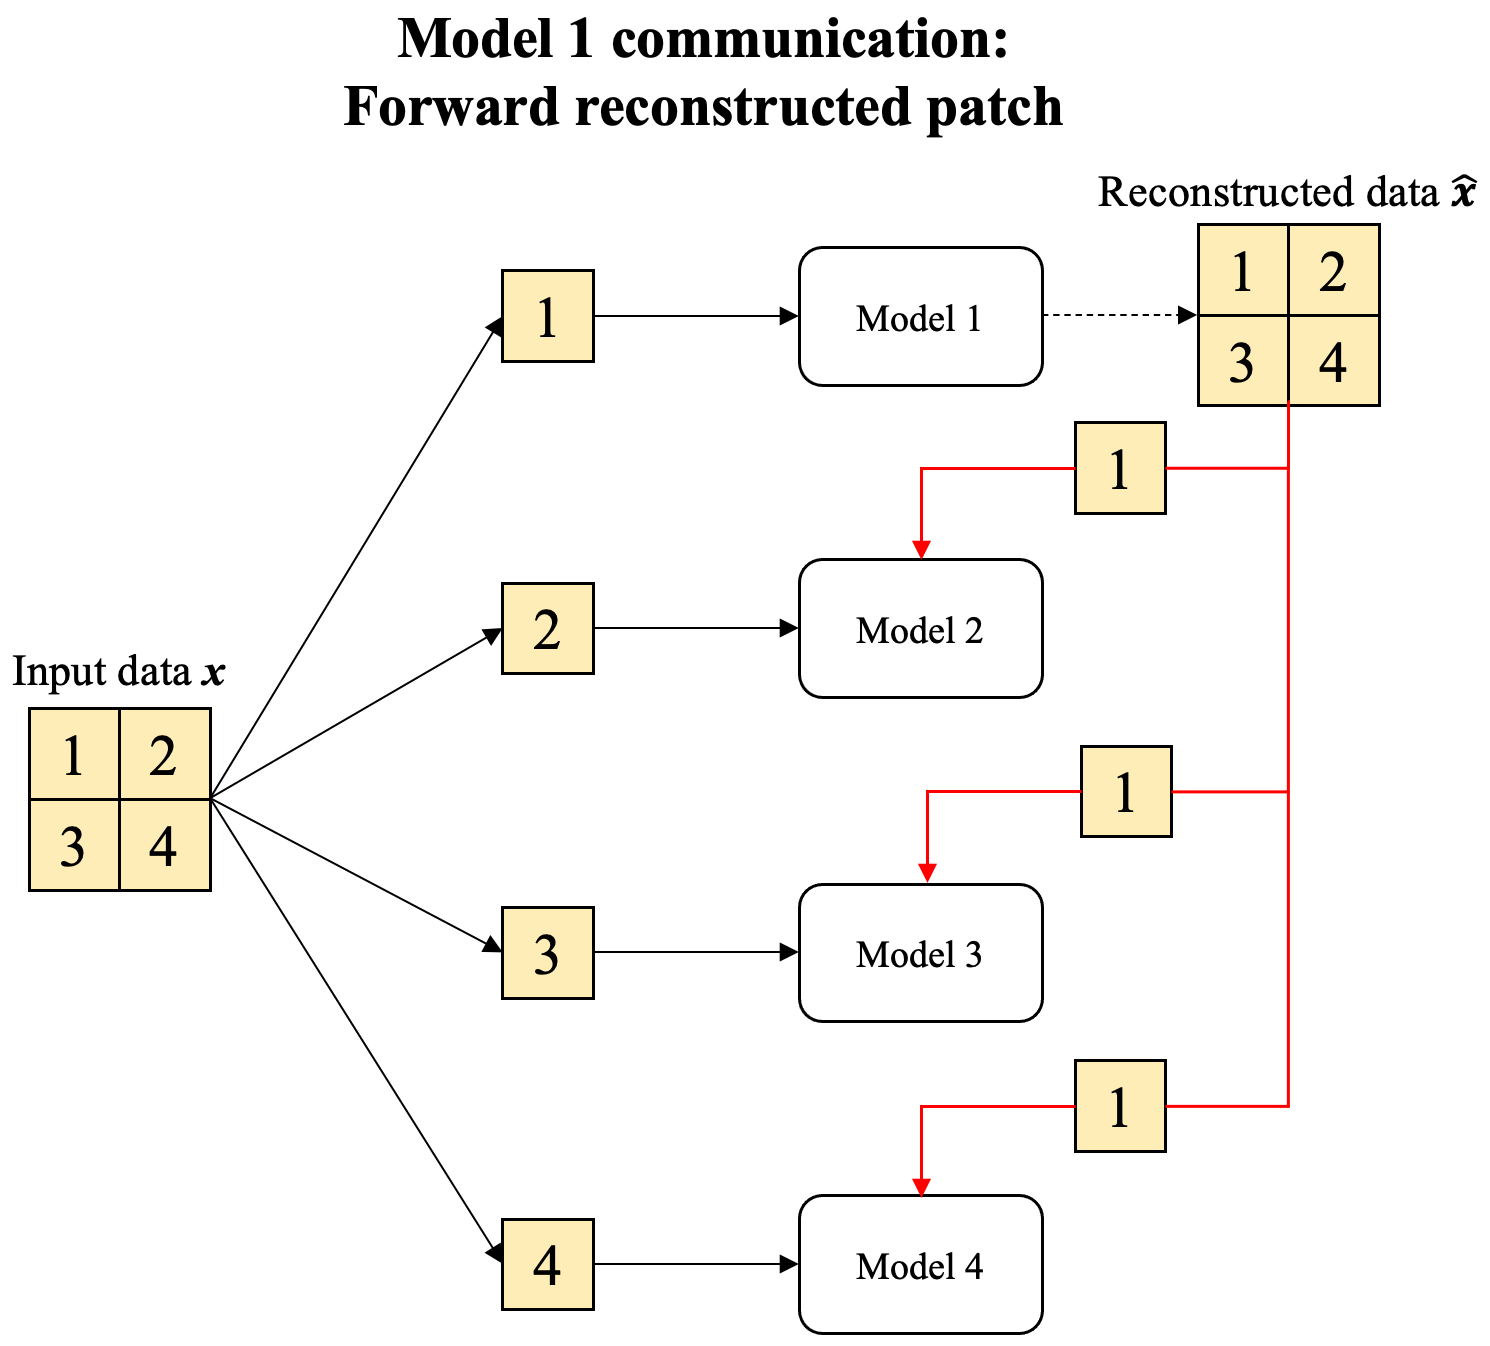
\includegraphics[width=0.80\textwidth]{recon_patch_forw}
    \caption[Communication between VAEs by forwarding reconstructed patch]{Communication between VAEs by forwarding reconstructed patch, example on the basis of the first VAE: The first VAE predicts the image and forwards the reconstructed patch (the same patch that was fed into the model) to the other VAEs.}
    \figlbl{recon_patch_forw}
\end{figure}

\begin{figure}
    \centering
    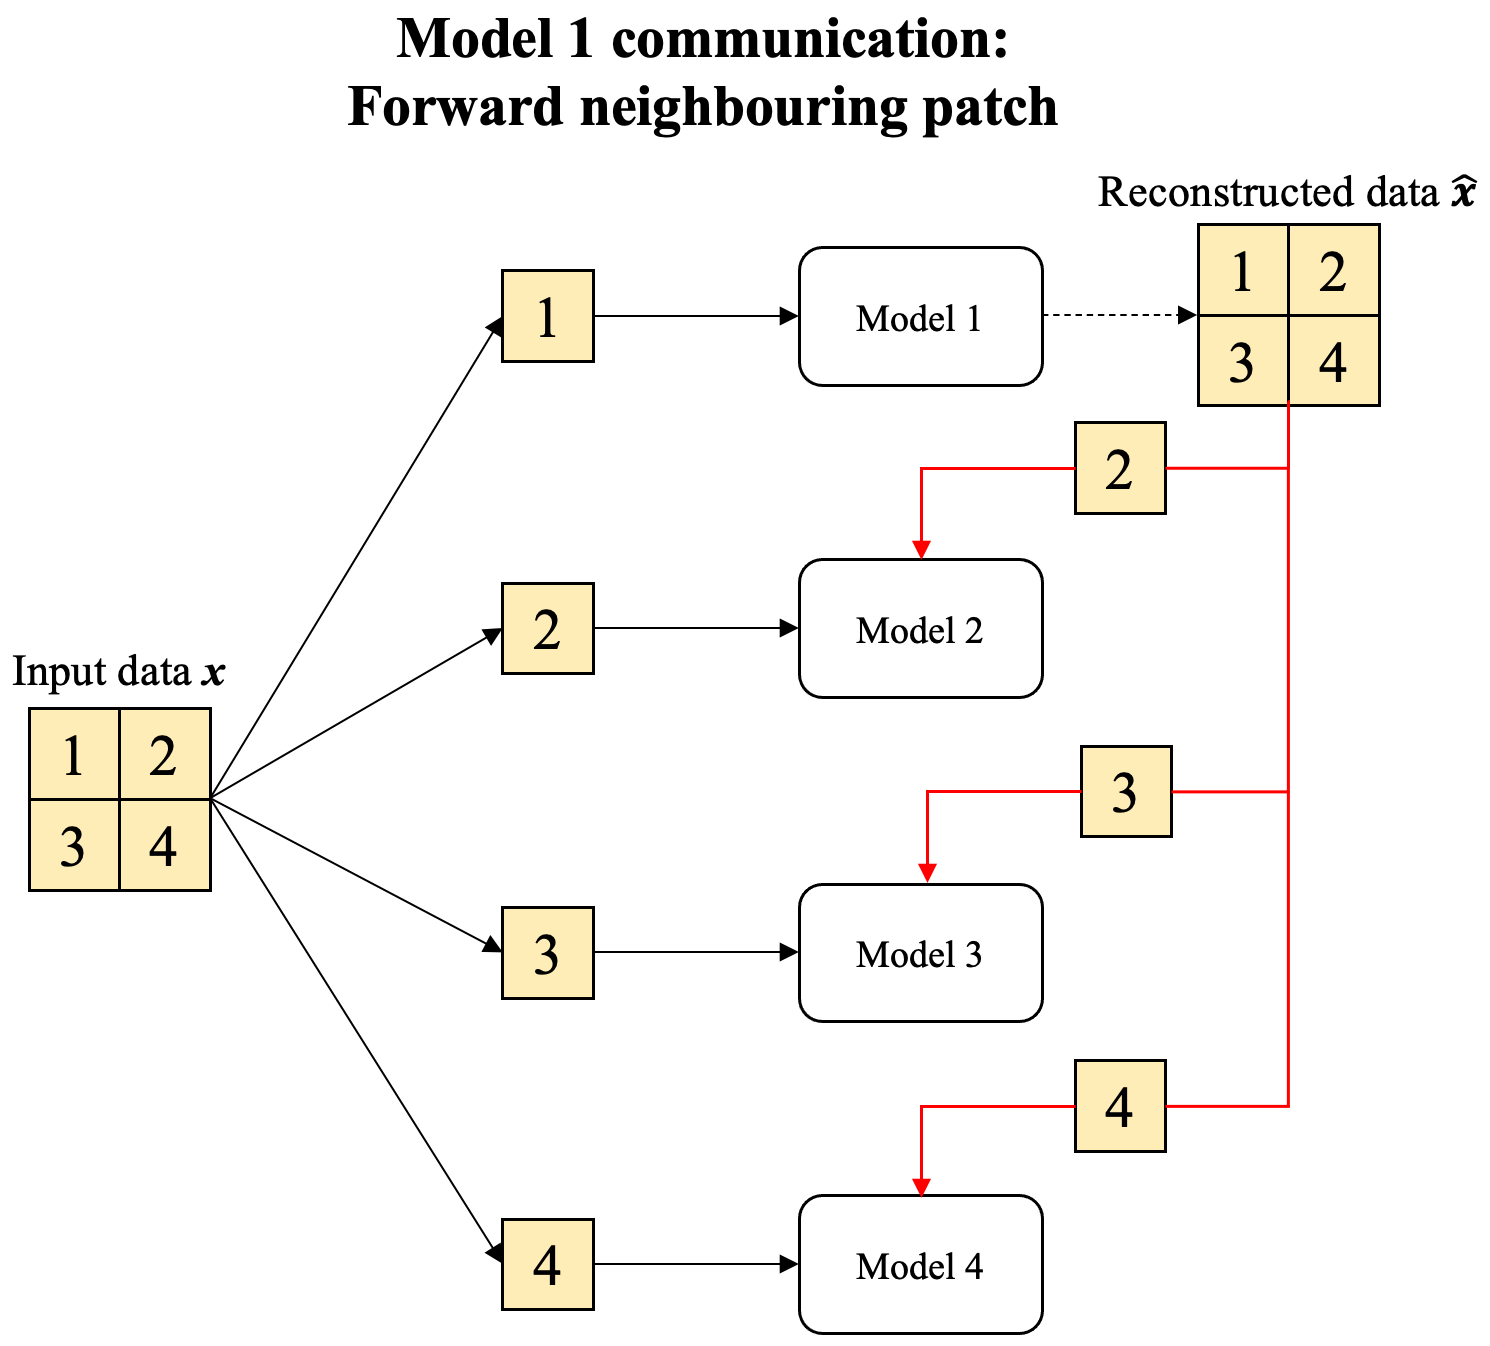
\includegraphics[width=0.80\textwidth]{neighbouring_patch_forw}
    \caption[Communication between VAEs by forwarding prediction of neighbouring patches]{Communication between VAEs by forwarding prediction of neighbouring patches, example on the basis of the first VAE: The first VAE predicts the image and forwards a prediction of how the neighbourhood could look like to the other VAEs. Thus, each other VAE receives a patch and a prediction of the first VAE how this patch could look like as input.}
    \figlbl{neighbouring_patch_forw}
\end{figure}

\begin{figure}
    \centering
    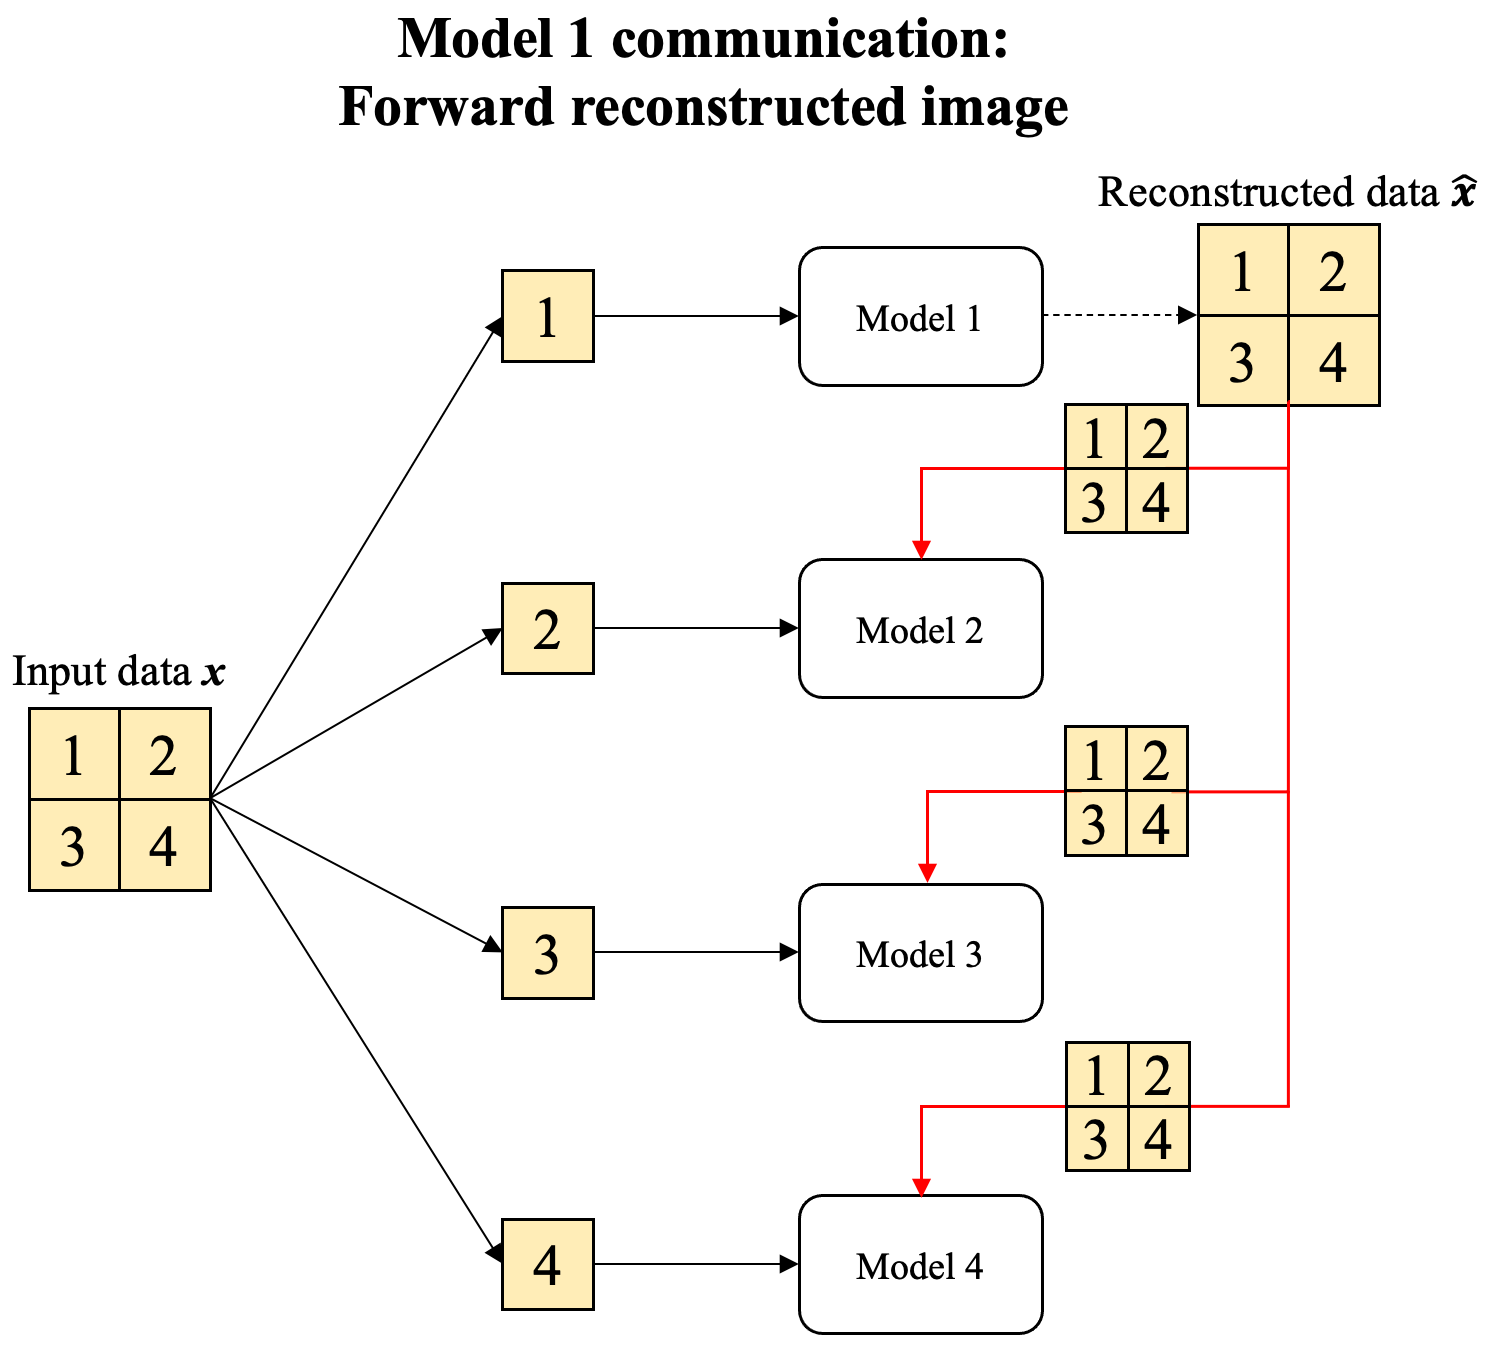
\includegraphics[width=0.80\textwidth]{recon_img_forw}
    \caption[Communication between VAEs by forwarding prediction of the entire image]{Communication between VAEs by forwarding prediction of the entire image, example on the basis of the first VAE: The first VAE predicts the image and forwards the prediction of the image to the other VAEs.}
    \figlbl{recon_img_forw}
\end{figure}



\begin{description}
	\item [Reconstructed Patch] Each VAE reconstructs its input patch and optionally a part of the neighbourhood. It tells the other VAEs what the reconstructed version of its input patch looks like. Information about the optionally reconstructed neighbourhood is not communicated to other VAEs. Thus, a reconstructed version of the input is sent to other VAEs and added as a new channel to their input. This process is exemplified for the first VAE in \figref{recon_patch_forw}. The problem with this approach is that in the first time-step all VAEs reconstruct their patch and the reconstructed version is communicated to the neighbouring VAEs. As a result, in the second time-step, each VAE receives information about the entire image and thus has access to global instead of only local image information\sidenote{even with a very large number of VAEs and communication restricted to the local neighbourhood, information about the entire image propagates to all VAEs over time, provided enough time-steps are executed}.  
	\item [Neighbouring Patch] Instead of communicating the reconstructed input patch to the neighbours, a prediction can be made of what the input patch of the neighbour looks like and this prediction can be communicated. This has the advantage that each UAE receives different versions of the same patch as input and thus has no global image information. This process for the first VAE is visualised in \figref{neighbouring_patch_forw}. Intuitively, this can solve the following problem: If a VAE cannot decide which digit to predict, neighbouring VAEs can help it by predicting its input patch in a form that is more similar to one of the digits and thus support the VAE by making its decision. 
	\item[Entire image] The simplest version is when each VAE predicts the entire image and communicates this to all other VAEs. In the first time-step, only local information is available, in the second time-step, various predictions of how the image could look are additionally provided. Each VAE can then correct its own prediction based on these predictions of the other VAEs. This process is represented in \figref{recon_img_forw}. Identical to ``reconstructed patches'', global image information is made available to each VAE. This problem can be alleviated if for each VAE $i$ that receives the input patch $\boldsymbol{x}^{(i)}$, the part from its prediction of the whole image corresponding to $\boldsymbol{x}^{(i)}$ is masked. Otherwise, an input patch of a VAE is fed through the encoder and decoder and then communicated to the other VAEs. Then implicitly reconstructed data and not just neighbourhood predictions gets to each VAE as input. 
\end{description}



\subsubsection{Communication Channel}
Another way to communicate is through a dedicated communication channel. For this purpose, each VAE has not only $1$ input and $1$ output channel but $4$ input and output channels. The input patch is fed into the first channel and a reconstructed version of it is predicted in the first output channel. This corresponds to a classic VAE and the loss function remains identical.
The remaining three channels are for communication: Each VAE generates a separate communication output for its $3$ neighbouring VAEs on the remaining $3$ channels. Each of these channels is then stacked to the input of the corresponding VAE. For example, the first VAE receives a given patch on the input channel $1$ and communication data from the 2nd, 3rd, and 4th VAE on the input channels $2$-$4$. Based on this information, it outputs a reconstruction of the patch on the output channel $1$ and communication data to the 2nd, 3rd, and 4th VAE on the output channels $2$-$4$. Thus, there is a dedicated two-way communication channel between each neighbouring VAE. This is shown in \figref{vae_comm_channel}.


\begin{figure}[h]
    \centering
    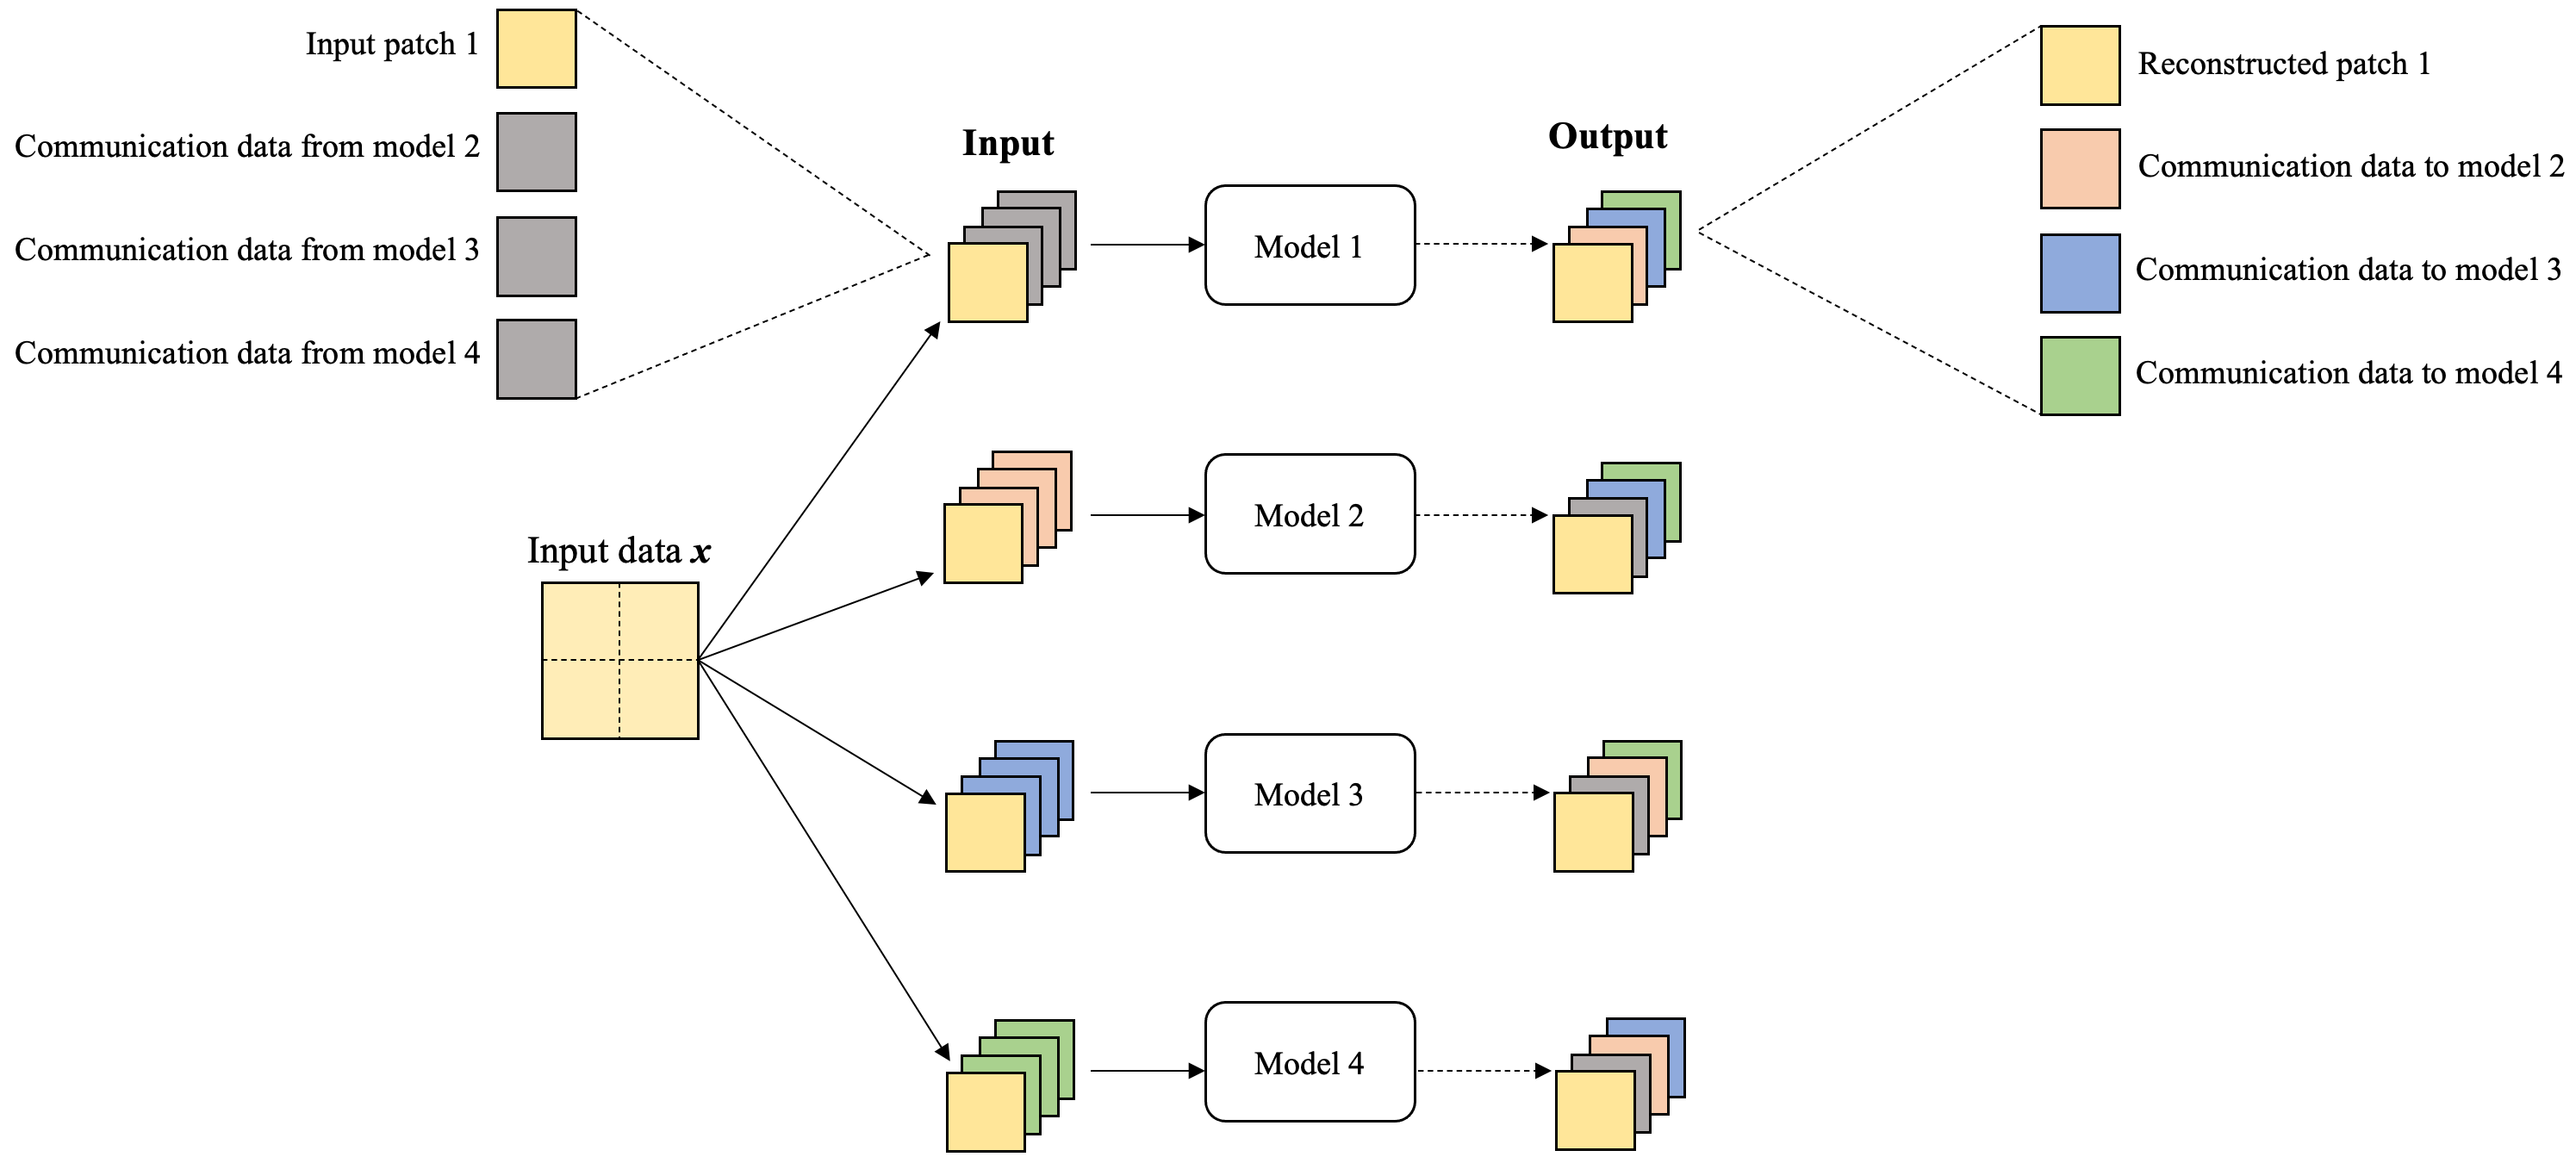
\includegraphics[width=0.89\textwidth]{vae_comm_channel}
    \caption[Communication between VAEs with a dedicated communication channel]{Each VAE has one and output channel to receive and reconstruct a given image patch. The other input and output channels are used for communication: Each VAE has for each other VAE a separate output channel to send messages and an additional input channel to receive messages.}
    \figlbl{vae_comm_channel}
\end{figure}

The loss function remains the same for the first output channel since the goal is still the same, i.e. to reconstruct the output as good as possible. The only difference is that model can now access $4$ input channels to reconstruct the input instead of one channel. However, the communication channels must be trained in order for them to be helpful for input reconstruction. Therefore, an additional loss term is applied on the $3$ output communication channels. Thereby, the idea is to optimize the output of these communication channels in a way so that the other VAEs can better reconstruct their patch.

Let $V = {V_1, ..., V_n}$ be the set of $n$ VAEs. Each VAE has $n$ output channels, one channel for the reconstructed image and $n-1$ channels for communication. Furthermore, each VAE $V_i$ has a loss $L_{\text{VAE}_i}$ based on the reconstruction goodness and the shape of the latent space (c.f. \eqref{hso_6}). The $3$ communication channels of a VAE $i$ can influence the loss $L_{VAE_j}$ of VAE $j$ (i.e. help to improve the loss by providing better information). How helpful the communication channels are can therefore be determined by the average of the loss of the other VAEs.

\begin{equation}\eqlbl{hso_9}
	L_{c_i} = \frac{1}{n-1} \sum_{n}^{j=1} L_{\text{VAE}_j} \text{, if } i \neq j
\end{equation}

Thus, the loss of a VAE with communication channel is

\begin{equation}\eqlbl{hso_10}
		L_{{\text{VAE}_C}_i} = L_{\text{VAE}_i} + \beta \cdot L_{\text{KLD}_i} + \beta_2 \cdot L_{c_i}
\end{equation}

where $\beta_2$ is a weight factor for the communication channel. Thus, each model optimizes its own reconstruction error, the shape of the latent space, and tries to improve the latent space and reconstruction error of other VAEs.


TODO: This has not been implemented yet (therefore, not explained in more detail).


\subsection{Class Prediction}
The VAEs are examined whether they are suitable for predicting the class label. To do this, all VAEs are first trained until they can reliably reconstruct images and the latent space is well formed.
After training, the average value of $\boldsymbol{\mu}$ is determined for each class $c \in C$ from the training set and each VAE $v$. This average value is called $\boldsymbol{\mu}_{\text{avg}_c}$ and is defined for $n$ samples as

\begin{equation}\eqlbl{hso_12}
		\boldsymbol{\mu}_{\text{avg}_vc} = \frac{1}{n} \sum_{i=1}^{n} \boldsymbol{\mu}_i
\end{equation}

This average value can be considered as the ``cluster centre'' of a class in latent space. In addition, $\boldsymbol{\mu}_{\text{avg}_vc}$ is a world model of a class. To make a prediction, a given sample is matched against these world models per class. As with vertical self-organisation, the cosine similarity between a sample and the class prototypes is used to determine their similarity. To predict a sample, first its $\boldsymbol{\mu}_vs$ is determined. Then, this sample is compared with all classes by computing the cosine similarity: 

\begin{equation}\eqlbl{hso_13}
		\text{cos}_{vsc} = \text{cos}(\boldsymbol{\mu}_vs, \boldsymbol{\mu}_{\text{avg}_vc}) = \frac{\boldsymbol{\mu}_vs \cdot \boldsymbol{\mu}_{\text{avg}_vc}}{\max(||\boldsymbol{\mu}_vs||_2, ||\boldsymbol{\mu}_{\text{avg}_vc}||_2)}
\end{equation}

Thus, the cosine similarity $\text{cos}_{vsc}$ between each class $c$' prototype and the sample $s$ is calculated for each VAE $v$.
Afterwards, the average class $c$ with the highest average cosine similarity between the sample activations $\boldsymbol{\mu}_vs$ and the class prototypes $\boldsymbol{\mu}_{\text{avg}_vc}$ is used as prediction.

\begin{equation}\eqlbl{hso_14}
		\argmax_{c \in C} \frac{1}{4} \sum_{v=1}^{4} \text{cos}_{vsc}
\end{equation}

Similar to vertical self-organisation, VAE's with a higher confidence have a higher cosine similarity between a class prototype and a specific class and thus have more influence on the class prediction than if the confidence is lower and the cosine similarity between the sample and all class prototypes is similarly large.

TODO: This has to be improved by also considering the standard deviation


TODO: Another improvement is to use multiple prototypes per class as digits may be written differently (depending on the person) and thus look different


\subsubsection{VQ-VAE}
In the case of classification, the latent space has to be shaped in a way that allows to assign a latent representation to a class.
This can be simplified if the encoder maps the input image to a discrete variable in the latent space.
Vector quantised variational autoencoders (VQ-VAE) \sidecite{NIPS2017_7a98af17} model such a discrete latent space by using vector quantisation (VQ).
Vector quantisation is a method that maps multi-dimensional vectors to a finite set of ``code''-vectors.
An image is fed into the encoder to obtain the encoder output $\boldsymbol{z}_e$.
Afterwards, a nearest neighbour lookup is made to find the code-vector that is most similar to $\boldsymbol{z}_e$.
The code-vector, also called the quantized vector $\boldsymbol{z}_q$ is fed into the decoder to reconstruct the image.


TODO: This has not been implemented yet (therefore, not explained in more detail).



\section{Results}\seclbl{horizontal_self_org_results}
As for vertical self-organisation (.c.f \secref{vertical_self_org_methods_dataset}), the MNIST \cite{Lecun_Bottou_Bengio_Haffner_1998} and MNIST-C \sidecite{Mu_Gilmer_2019} data sets are used to evaluate the models. 

Different models are trained to evaluate this architecture. A single VAE is used as the baseline (i), which receives the entire image as input and reconstructs it. This VAE is obviously trained without time steps and communication. Horizontal self-organisation is done using $4$ VAEs ($2\times 2$) in different settings: Four independent VAEs are trained (without time steps and communication), each VAE receives a non-overlapping image patch as input and either reconstructs the received patch (ii) or predicts the entire image (iii). Furthermore, different types of communication are investigated: The VAEs communicate the reconstructed \emph{input patch} to the other VAEs (according to \figref{recon_patch_forw}). This communication takes place over $4$ time steps and the VAEs are trained by either reconstructing the input patch (iv) or predicting the entire image\sidenote{but despite the prediction of the entire image, only the prediction of the reconstructed patch is communicated to the other VAEs.} (v). In another version, each VAE predicts the whole image and forwards the predicted \emph{input patch of the neighbour} to each VAEs over $4$ time steps  (vi) (c.f. \figref{neighbouring_patch_forw}). Finally, the VAEs are also used to predict the whole image over one time step and the \emph{predicted image} is forwarded to the other VAEs (e.g. \figref{recon_img_forw}) (vii). \tabref{hso_models} gives an overview of the models described.


\begin{table}[h] 
    \tablbl{hso_models}
    \centering
	 \begin{tabular}{l l l l l}
    	\textbf{No.} & \textbf{$n$ VAEs} & \textbf{Reconstruction} & \textbf{Communication} & \textbf{Time-Steps}\\
        \hline
		i & 1 & Image & -  & -\\
		ii & 4 & Patch & -  & -\\
		iii & 4 & Image & - & -\\
		iv & 4 & Patch & Input Patch & $4$\\ %p_diff
		v & 4 & Image & Input Patch & $4$\\  %p_diff
		vi & 4 & Image & Neighbouring Patch & $4$\\ %p_same
		vii & 4 & Image & Image & $1$\\
    \end{tabular}
    \caption[Different Models to Evaluate Horizontal Self-Organisation]{Different models for evaluating horizontal self-organisation: The first column shows a number used as a reference id in this thesis. The second column shows the number of VAEs used, the third column whether the input field or the whole image is reconstructed, the fourth column what is communicated to the neighbouring VAEs, and the fifth column over how many time steps the communication takes place.}
\end{table}

The number of time steps is a design decision: obviously, the models without communication do not need time steps. In the case where each VAE predicts the entire image and forwards it to the other VAEs, only one time step is used. This means that the entire image is predicted once and then forwarded to the other VAEs. It has been observed that one time step is sufficient and that the predictions do not change in further time steps. This could be due to the fact that all relevant information is already transmitted within one time-step and no further communication cycles are necessary. However, if only a patch of the image is forwarded to the other VAEs, the predictions may change over several time steps. In this thesis, $4$ time steps are used when only patches are forwarded to the other VAEs. It is observed that the predictions usually do not change after $4$ time steps and thus using $4$ time steps seems enough. When only patches are forwarded, the model contains much more dynamics: a VAE predicts something, communicates it to its neighbours and receives data from its neighbours. In a subsequent time step, the VAE has more information and can correct its prediction, which in turn can lead to a correction of a neighbour's prediction. Thus, the communication occurs over several time steps in which the VAEs correct each other. An example of four predicted samples is shown in \figref{hso_over_time}: The left side shows the initial prediction of the model (vi) and the right side the prediction of the same image after $4$ time steps. This visualisation indicates that the predictions are improved thanks to the communication. The investigation of the reconstruction error confirms the efficiency of the communication: The initial prediction without communication has an average reconstruction error of $0.23$, and the prediction after $4$ time step has an error of $0.16$.

\begin{figure}[h]
    \centering
    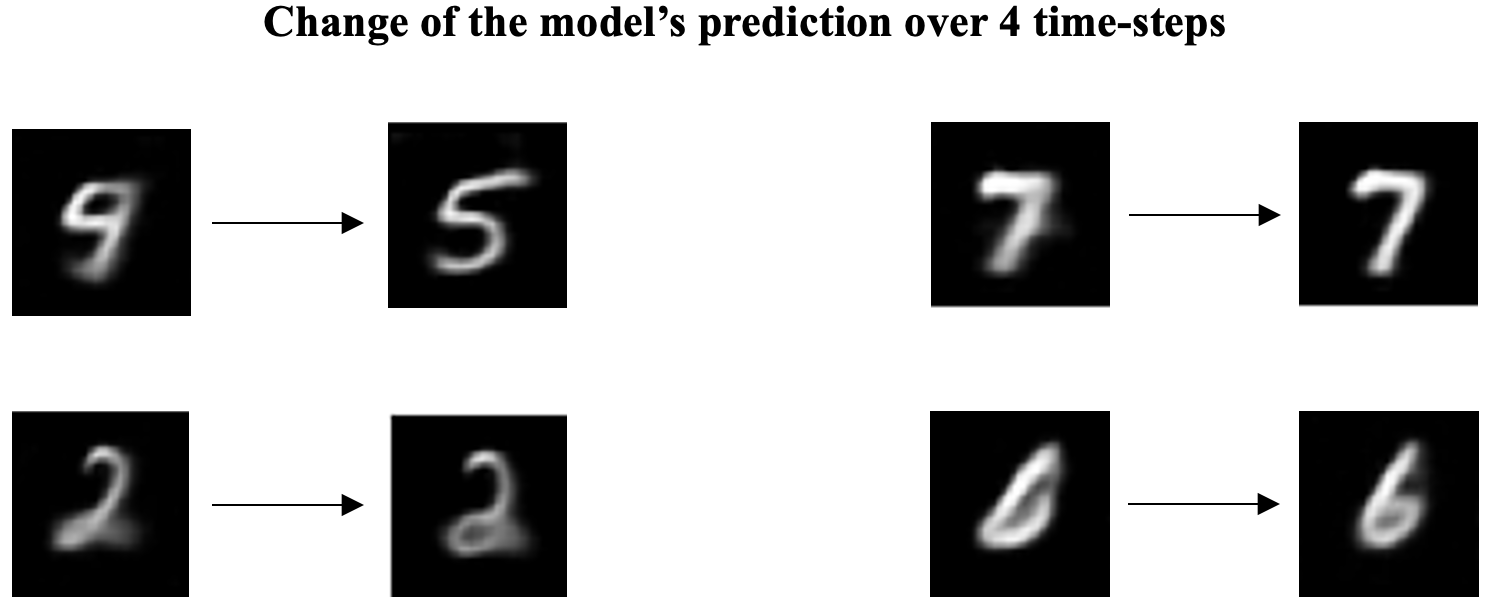
\includegraphics[width=0.79\textwidth]{hso_over_time}
    \caption[Change of the model's prediction over time]{Four random predictions of model (vi) over $4$ time-steps: The initial prediction is shown on the left and the prediction after $4$ communication cycles on the right.}
    \figlbl{hso_over_time}
\end{figure}

Of particular interest in this evaluation is not how well the samples are reconstructed but how well the latent space is shaped. Visualising the $\boldsymbol{\mu}$ values is a simple way to investigate the latent space. Therefore, the $\boldsymbol{\mu}$ vectors with a length of $n=32$ are reduced to $2$ dimensions using t-SNE \sidecite{van2008visualizing} and visualised. Since $25$ VAEs are trained in this evaluation, visualising all t-SNE plots is infeasible. Instead, \figref{hso_tSNE} only shows the plot of the baseline, the plot of the model (ii) as an example of an architecture without communication, and the plot of the model (vi) as a representative example of an architecture with communication. 

As expected, the latent space of model (i) is relatively well organised and the classes are distinguishable within the latent space. In this model, only one VAE is used, which receives the entire image as input which simplifies the organisation of the latent space. Model (ii) consists of $4$ VAEs without communication. Its latent space is less well organised: the classes are no longer clearly identifiable as clusters. However, it is interesting to note that each VAE can separate certain classes better than others because of the different patch it receives as input. Considering all $4$ VAEs, each class can be relatively well identified by at least one VAE, while no VAE can identify all classes. This indicates the benefit of a communication between the VAEs.
Applying the proposed measures (i.e. communication and predicting the whole image instead of reconstructing the input patch), the arrangement of the latent space for each VAE improves significantly: almost every VAE is able to separate the classes. This supports the usefulness of the proposed measures.

\begin{figure}[h]
    \centering
    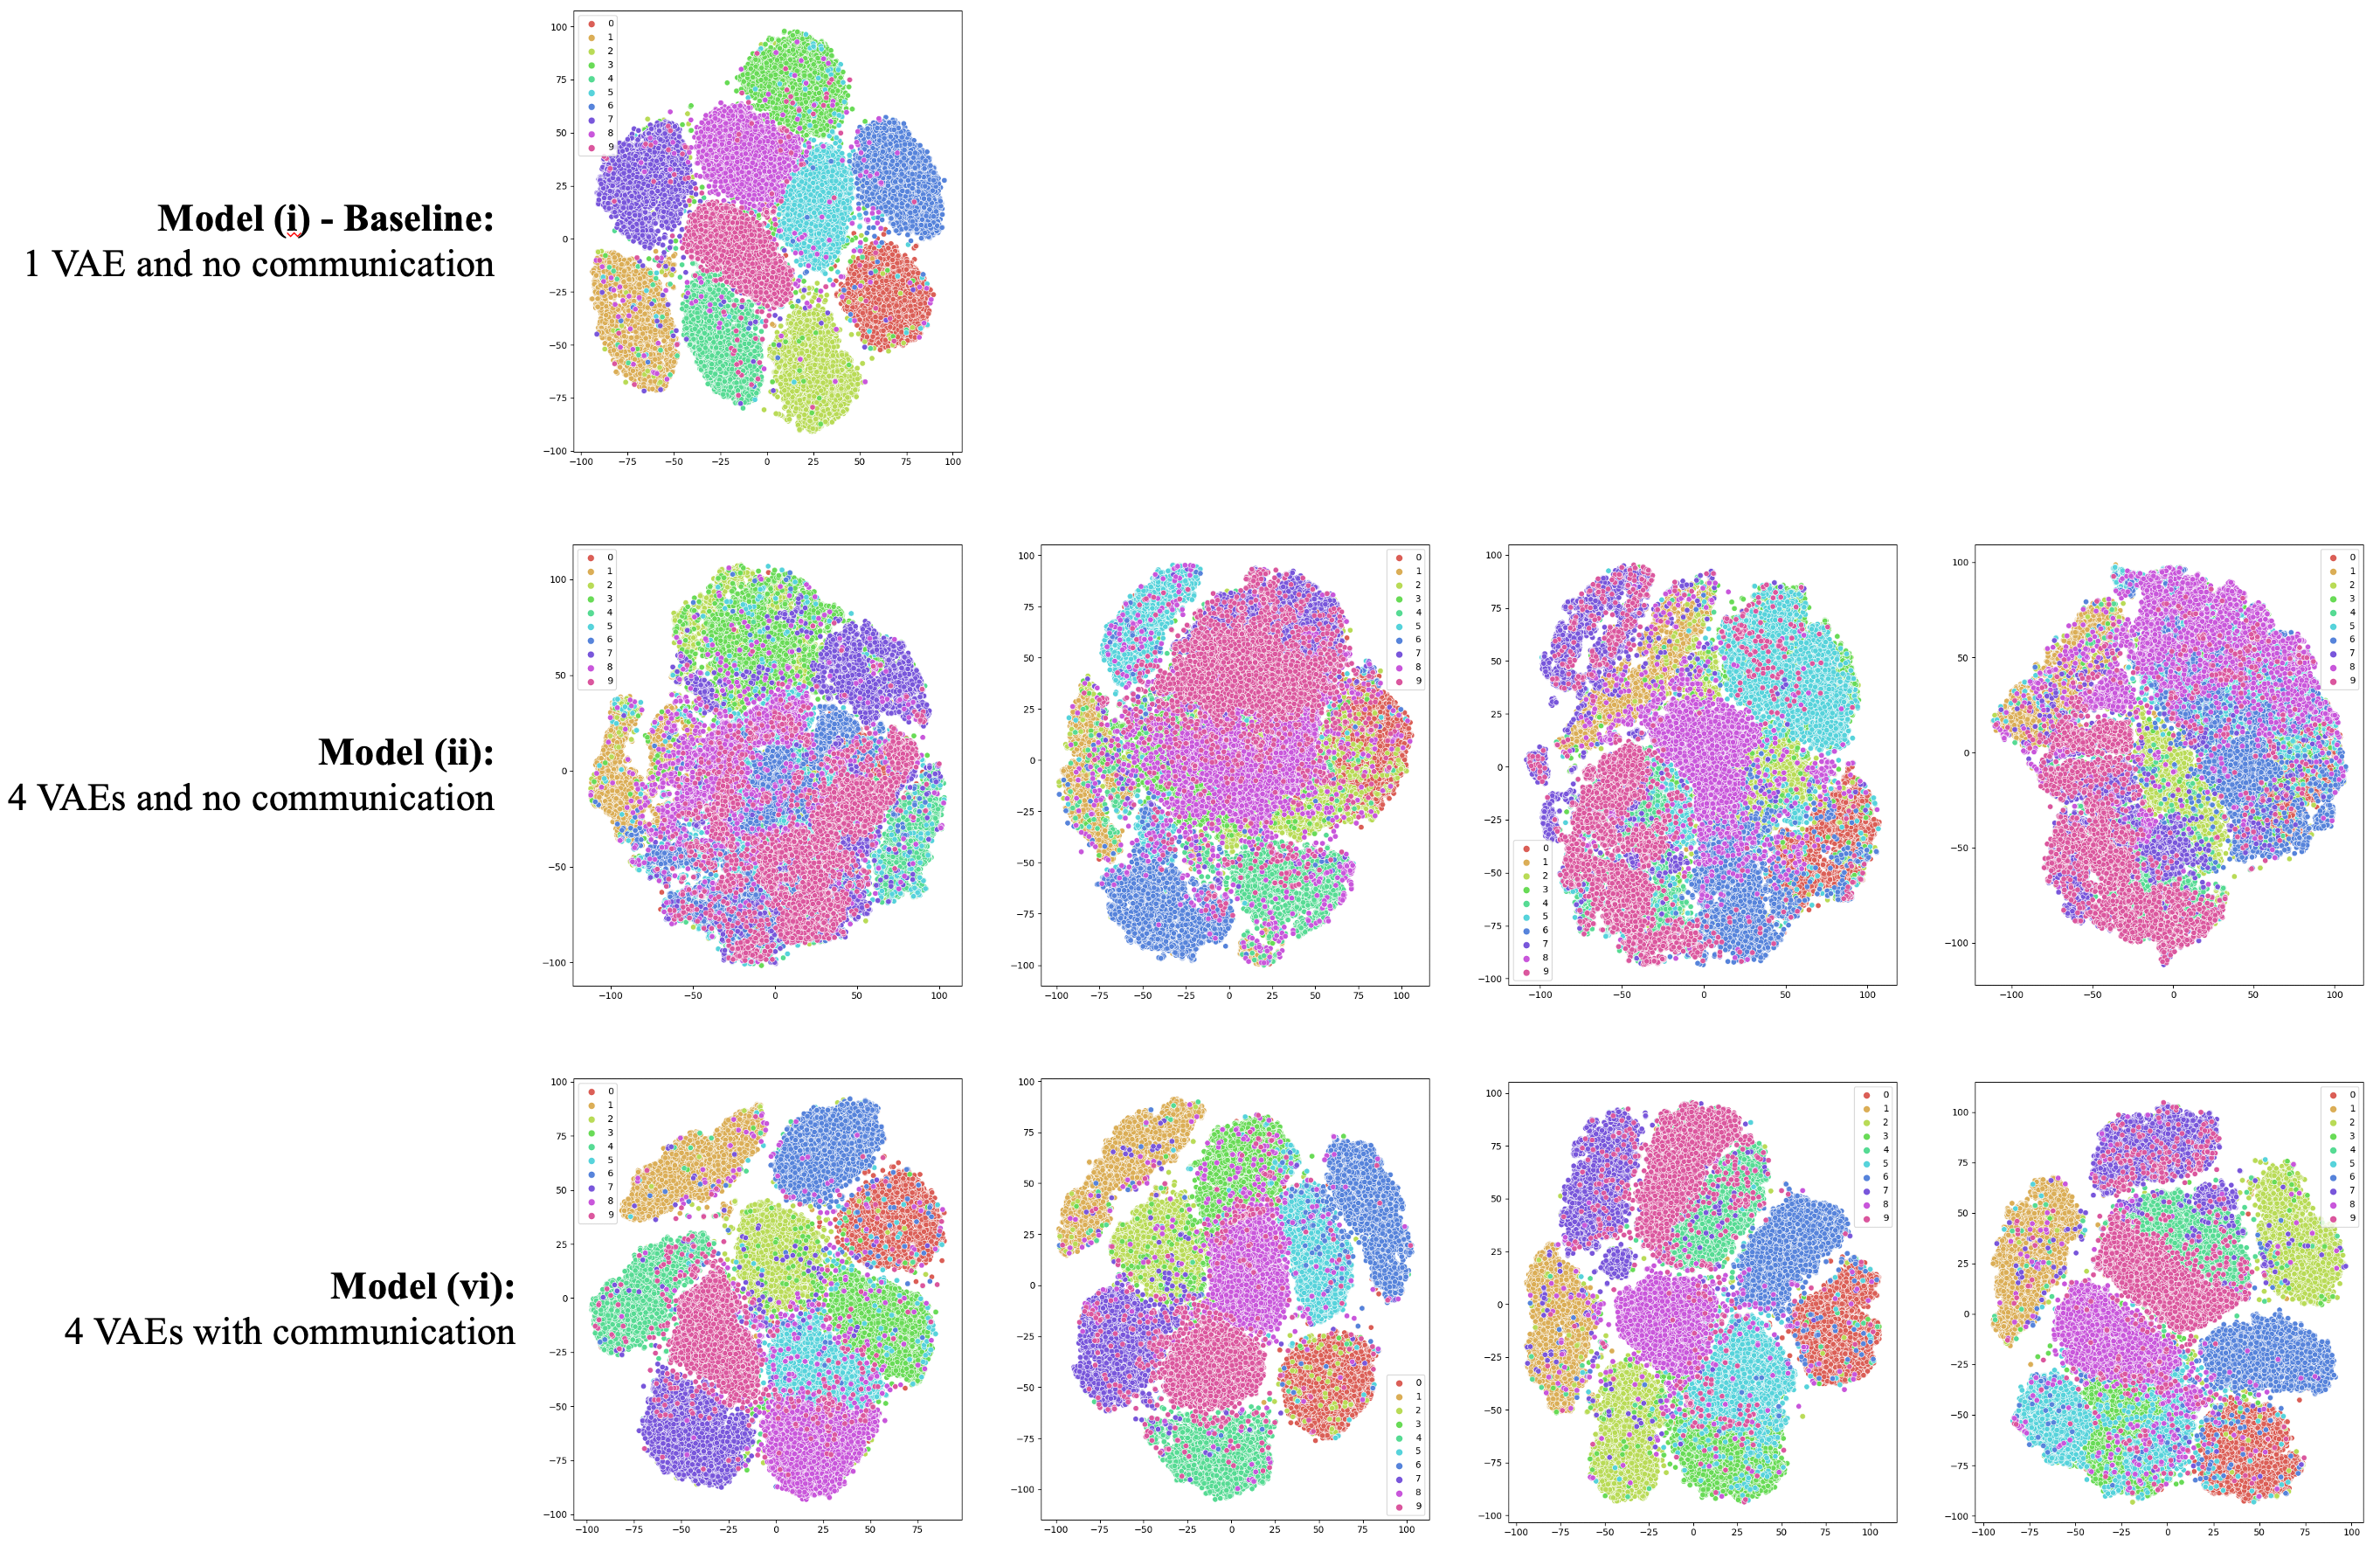
\includegraphics[width=0.99\textwidth]{hso_tSNE}
    \caption[t-SNE plot of the $\boldsymbol{\mu}$ values of different models]{t-SNE plot of the $\boldsymbol{\mu}$ values of four different models: The first row shows the baseline model ($1$ VAE), the second row the model (ii) that consists of $4$ VAEs without communication, and the third row the model (vi) that uses $4$ VAEs with communication channels. Each point in the plot corresponds to a sample, the samples are coloured according to their class.}
    \figlbl{hso_tSNE}
\end{figure}


Another way to evaluate the latent space is to measure its suitability for classification. This can be done by applying a k-means clustering and then calculating the normalised mutual information (NMI) score between the cluster centres and the labels. This metric allows the comparison between cluster assignments and labels by calculating the consistency. This means that it measures how clearly a cluster can be assigned to a label. \tabref{hso_nmi} shows the NMI scores of the models.
The NMI score is difficult to interpret as a number, and it is unclear exactly what, for example, a score of $0.6$ means for model (i). However, a relative comparison of the scores is of interest for this evaluation. The model (i) is a single VAE that receives the entire image as input, not just a patch of it. Therefore, this model is assumed to have a well-formed latent space, and the value of $0.6$ is close to an upper bound for a good latent space in this setting.

It is evident that the latent space is significantly better shaped when the whole image is predicted and not only the input patch is reconstructed. For example, models (ii) and (iii) as well as (iv) and (v) are the same models but one of the models reconstructs the input patch and the other one predicts the entire image. The models that predict the whole image are significantly better: the NMI value increases on average from $0.36$ to $0.53$ (model (ii) $\rightarrow$ model (iii)) and from $0.37$ to $0.59$ (model (iv) $\rightarrow$ model (v)) respectively.

A slight improvement through communication can also be observed. Model (iii) consists of $4$ VAEs without communication and predicts the whole picture. It achieves an NMI value of $0.53$. The models with communication are all better, reaching NMI values of $0.59$ (model (v)), $0.54$ (model (vi)) and $0.54$ (model (vii)). However, the improvement is not as clear as for the prediction of the whole image. This is probably due to the fact that the image patches are too large and more VAEs should be used. For example, model (iii) has a very high NMI score compared to the baseline, indicating that this model is able to classify and therefore the image patches contain too much image information. This makes communication less important and the results are not significantly improved by adding communication.


\begin{table}[h] 
    \tablbl{hso_nmi}
    \centering
	 \begin{tabular}{l l l l}
    	\textbf{No.} & \textbf{Avg. NMI} & \textbf{Min. NMI} & \textbf{Max. NMI}\\
        \hline
		i & $0.60$ & $0.60$ & $0.60$ \\
		ii & $0.36$  & $0.29$ & $0.39$ \\
		iii & $0.53$ & $0.49$ & $0.56$ \\
		iv & $0.37$ & $0.33$ & $0.41$\\
		v & $0.59$ & $0.58$ & $0.61$ \\
		vi & $0.54$ & $0.49$ & $0.60$ \\
		vii & $0.54$ & $0.49$ & $0.59$\\
    \end{tabular}
    \caption[NMI score of different architectures]{The NMI score between the $\boldsymbol{\mu}$ cluster centres and the ground-truth label. The clusters are calculated by using the k-means algorithm. Most models consist of several VAEs, therefore the average, minimum and maximum NMI values are reported for all VAEs per model.}
\end{table}

Finally, the proposed classification method is evaluated. For this purpose, the accuracy on the MNIST and MNIST-C data sets is determined for each model. The results are shown in \tabref{hso_accuracy}.
For each VAE of a model, the cosine similarity according to \eqref{hso_13} between a sample and a class prototype is calculated. Thus, the accuracy can not only be calculated for the entire model (i.e. all $4$ VAEs together), but also for each VAE independently. \tabref{hso_accuracy} shows the average accuracy per VAE in the column ``Avg. VAEs''. Furthermore, by calculating the average cosine-similarity a voting over all VAEs is performed and the actual model accuracy os obtained. The accuracy of this voting is shown in the column ``Overall''. The voting works exceptionally well: for example, model (ii) has $4$ VAEs with an average accuracy of $62.4\%$ on the MNIST dataset. The best VAE has an accuracy of $66.1\%$, the worst $59.7\%$. By voting, the overall accuracy increases to $81.7\%$, which is significantly better than the best VAE.

On the MNIST data set, the base model (i) is significantly outperformed by some models in terms of accuracy, but robustness (measured on MNIST-C) is not significantly improved by using multiple VAEs. As with the evaluation of the NMI score, it can be observed that models that predict the entire image perform better than models that only reconstruct a patch of the image. Furthermore, the accuracy of the models without communication is generally very high, suggesting that the image patches are too large and more VAEs should be used.



\begin{table}[h] 
    \tablbl{hso_accuracy}
    \centering
	 \begin{tabular}{l l l l l}
	 	& \textbf{Avg. VAEs} & \textbf{Overall} & \textbf{Avg. VAEs} & \textbf{Overall}\\
    	\textbf{No.} & \textbf{MNIST} & \textbf{MNIST} & \textbf{MNIST-C} & \textbf{MNIST-C}\\
        \hline
		i & - & $85.2\%$ & - & $63.4\%$ \\
		ii & $62.4\%$ & $81.7\%$ & $42.3\%$ & $60.9\%$ \\
		iii & $78.2\%$ & $89.9\%$ & $45.4\%$ & $64.9\%$ \\
		iv & $63.8\%$ & $82.6\%$ & $41.8\%$ & $60.5\%$  \\
		v & $86.1\%$ & $87.6\%$ & $62.4\%$ & $65.2\%$ \\
		vi & $88.4\%$ & $91.1\%$ & $50.4\%$ & $59.2\%$ \\
		vii & $78.5\%$ & $90.0\%$ & $46.8\%$ & $64.2\%$ \\
    \end{tabular}
    \caption[Accuracy of different architectures on MNIST and MNIST-C]{The accuracy of different models on MNIST and MNIST-C. For both data sets, the average accuracy per VAE and the overall accuracy is reported. The average per VAE is the average accuracy when each VAE makes a prediction on its own (i.e. choosing the highest cosine similarity per VAE according to \eqref{hso_13}). The overall accuracy is calculated by averaging the cosine similarity according to \eqref{hso_14}.}
\end{table}

The accuracy was calculated by comparing a sample with \emph{one} prototype per class. However, using only one prototype seems to be not enough. For example, when looking at the t-SNE plots in \figref{hso_tSNE}, the same class is divided into more than one cluster. The calculation of the NMI score also indicates that one prototype per class is insufficient: When more clusters are used for k-means clustering, the NMI scores become higher. This is also in line with the analysis of the data and the findings of vertical self-organisation (c.f. \secref{future_vso}).



TODO: Model Head is missing in this evaulation




%TODO: vereinheitliche Mathe: Was ist underline, was ist hochgestellt in Klammern ($z^{(i)}$) und was ist hochgestellt in eckigen Klammern? Bei NN: Was ist n, was ist m, ... (+ Lernraten Symbol, Loss Symbol, etc.)
%Sind alle Vektoren bold?

% TODO: target function und objective function vereinheitlichen
% TODO: net-fragment or net fragment, dataset or data set, time-step or time step



\setchapterpreamble[u]{\margintoc}
\chapter{Future Work \& Conclusion}\chlbl{future_work}
\section{Discussion}
Deep learning networks have demonstrated their exceptional capabilities as feature extractors. 
Recent advancements in scaling have brought them to a level where they hold the potential for widespread applicability across various tasks in our everyday lives.
Nevertheless, they have intrinsic limitations, and the prospect of overcoming these barriers remains uncertain.
This thesis presents a vision framework that addresses several of these challenges, primarily focusing on mitigating early commitment and facilitating object-agnostic transformation invariance.

The proposed framework is strongly inspired by the biological brain, the only known system to which we attribute true intelligence.
One of this thesis's main contributions is identifying neuroscientific findings and their subsequent integration within the contours of a computational framework.

A key difference between the proposed system and deep networks is that deep learning lies in the mechanism of building consistency:
Deep networks optimise consistency at a single point in the network by comparing its prediction with a teaching signal.
A global error correction algorithm such as backpropagation adjusts all components in the network to minimise inconsistencies at a single point.

In contrast, the proposed framework implements a model that optimises consistency at every point in the network, akin to the human brain.
It encompasses three building blocks, all using binary Bernoulli neurons.
These biologically plausible neurons allow net fragments to be implemented and improve robustness. However, their full optimisation within the prevailing computational framework remains an ongoing endeavour.

The sensory stage \emph{S0} corresponds in the biological context to the eyes and extracts features from images.
The implementation could involve the first convolutional layer of a pre-trained autoencoder. Given the well-established feature extraction capabilities of CNNs, it is reasonable to expect the suitability of this layer without having done extensive experiments within this thesis.

The feature building stage \emph{S1}, inspired by the primary visual cortex, leverages lateral connections to form net fragments, groups of neurons that support each other's activity.
This stage is well examined in this thesis and iteratively refined based on empirical investigations.
The experiments confirm the usefulness of lateral connections in tasks such as occluded object reconstruction and noise reduction.

The prototype stage \emph{S2} takes inspiration from the ventral visual stream and the temporal cortex.
It uses projection fibres to map network fragments onto object prototypes. While this aspect is well explained theoretically in this thesis, it lags behind \emph{S1} in empirical validation and refinement.


At its core, the entire network is based on the principles of self-organisation, locality and cell consistency.
Network fragments arise from cells communicating with their spatial neighbours, while projection fibres connect neighbouring cells in \emph{S1} and \emph{S2} and seek consistency with neighbouring fibres.
These basic principles are fundamentally different from existing deep networks. In addition, the network incorporates constraints aimed at reducing early commitment and increasing robustness. The iterative process of assembling net fragments and mapping them to object prototypes leads to transformation-invariant feature processing independent of specific objects.

In summary, the proposed framework introduces several promising principles. However, as elaborated in the next section, these principles must be explored and refined further in future work.
Comparing the proposed framework with deep networks is not possible at its current stage as it is far from being developed enough. 
I speculate that deep networks excel at well-defined tasks that can be measured with corresponding metrics because they optimise all network neurons to maximise consistency between a prediction and a task-specific teaching signal at a single network node. Conversely, optimising the consistency at every single point in the network, as done in the proposed framework, might be a way towards more intelligent systems. Such a configuration could harmonise different signals, each contributing to coherent representations in the decision-making processes. By doing so, each signal and cell would cast its vote for a particular course of action and seek consensus without an external source providing a global teaching signal.


\section{Future Work}
This work is a preliminary study for a possible dissertation, focusing on refining the proposed framework.
Consequently, numerous avenues exist for future work to improve the proposed framework. The following section outlines some of the most pressing issues and proposes the next steps.


\subsection{Alternative Cells in \emph{S1}}\seclbl{future_alt_cells}
In the context of \emph{S1}, individual cells represent distinct features that are localised in a specific spatial location. These cells support each other's neuronal activity. As outlined in \secref{framework_neuroscience}, these cells can contribute to mutually exclusive net fragments. For example, cell $A$ may participate in a fragment with cell $B$ and another fragment with cell $C$, while cell $B$ and $C$ avoid simultaneous activation. This exceeds the functional capacity of cell $A$, and a copy of $A$ is needed to establish separate lateral connections with cell $B$ and $C$.

The \secref{framework_alt_cells} described that alternative cells could be implemented by duplicating the output channels of the weight matrix $\boldsymbol{W}$ of \emph{S1}.
Alternative cells contribute to different net fragments and are mutually exclusive.
Consequently, competition between these alternative cells is required to ensure that only a winning cell can become active and that activity in alternative cells is suppressed\sidenote{Activity can be suppressed by inhibition, as it is already implemented in \emph{S1}.}.

Preliminary experiments suggest that the initially similar characteristics between alternative cells make it difficult to establish effective competition and that this initial symmetry that needs to be broken first.
Introducing controlled randomness during the initial phase could increase the stochasticity of the learning process. This randomness can potentially enhance differentiation and separation between these different cells.

Furthermore, an extension of Hebbian learning is needed to enable the forgetting of previously learned patterns.
Currently, each update only increases the weights, which strengthens lateral support.
However, some updates could inadvertently create incorrect connections between different (alternative) cells.
The following section describes negative Hebbian learning, a mechanism that allows forgetting learned connections and seems crucial to implementing alternative cells.
This mechanism eliminates the need to carefully prevent false updates during the initial training phase, as erroneous updates can be corrected as soon as the alternative cells are separated enough.

\subsection{Negative Hebbian Learning within \emph{S1}}
The previous section describes how negative Hebbian learning can help to realise alternative cells.
While conventional Hebbian learning increases the synaptic weights between simultaneously active neurons, negative Hebbian learning introduces a complementary process by decreasing the synaptic weight between cells that fire disjoint.
These negative updates are not only crucial in the formation of alternative cells but also in gradually eliminating less significant patterns that have been imprinted during the training phase.

Implementing negative Hebbian updates is challenging, especially when the data is dominated by negative correlations\sidenote{The dataset contains more samples where two feature cells are active separately than simultaneously.}, as shown in \chref{neg_hebb_updates}.
One possible strategy to overcome this problem is using a significantly lower learning rate for negative updates than for positive ones.
This asymmetry ensures that the process of forgetting is slower than the process of learning, preventing the abrupt erasure of acquired patterns.
Another solution is alternative cells: If two patterns have a positive correlation at one point and a negative correlation at another point (as in the example shown in \chref{neg_hebb_updates}), these patterns can be processed differently by employing alternative cells, effectively maintaining their distinct representations.


\subsection{Refine \emph{S2}}
An important task for future work is the empirical improvement of \emph{S2}, which has only been theoretically developed based on identified neuroscientific findings. The current blueprint describing its implementation has to be further refined by conducting experiments.

In the first phase, the integration and evaluation of projection fibres based on shifter circuits \sidecite{anderson_shifter_1987, olshausen_neurobiological_1993} should be done and explored within the proposed framework.
During this process, also different object views should be explored (provided by the medium processing loop). Currently, these views are only used during evaluation, but once \emph{S2} is implemented, they can be crucial in learning to associate different views to the same prototype, encouraging transformation-invariant mappings.

Once an initial effective mapping has been created, the presumed simplifications can be avoided (c.f. \secref{framework_s2}). In particular, novel prototypes from unseen objects can be stored automatically, the prototypes can be iteratively improved throughout training, projection fibres can be learned dynamically, and the network can be extended to interpret complete scenes, thus going beyond the limits of object-centric images.






\subsection{Scaling to Different Datasets}
In the experiments, a dataset comprising straight lines is used, effectively illustrating the principles and enhancing understanding of the proposed framework.
Nevertheless, assessing the models' scalability to larger and more diverse datasets is important.
One possible avenue is to use traditional classification datasets such as MNIST \sidecite{lecun_gradient-based_1998}, CIFAR-10 \sidecite{krizhevsky_learning_2009}, or ImageNet \sidecite{russakovsky_imagenet_2015}.
However, it is important to note that the primary goal is not to push benchmarks for image classification.
Rather, the goal is to obtain high-quality object representations.

This endeavour may require building new datasets generated by an image rendering engine capable of simulating 3D objects and generating data in real-time.
Using such an engine allows to generate visualisation of objects undergoing realistic-looking transformations and depth rotations.
This method allows the evaluation of the model's ability to process complex and diverse visual data that more closely resembles real-world scenarios.
Moreover, these transformations are an integral part of the proposed processing loop and even allow interaction with objects. For example, the model could determine the optimal viewing angle when looking at an object and thus improve its representation to ensure internal consistency.




\subsection{Multi-Modality}\seclbl{framework_multi_modality}
This work focuses on a framework for computer vision. However, the architecture has broader applicability and can be used for processing different sensor signals and be used in multimodal settings \cite{ngiam_multimodal_2011, liu_learn_2018, baltrusaitis_multimodal_2019}.
Having similar cell architectures processing different kinds of signals is also in line with findings from neuroscience \sidecite{mountcastle_organizing_1978, mountcastle_columnar_1997}.

In the case of images, net fragments in \emph{S1} represent learned visual patterns that are part of an object's surface and are mapped with protection fibres to object prototypes that describe the visual appearance of objects. 
The same architectural structure can be applied to other types of signals. For example, an alternative sensory system could perceive audio signals. In this scenario, the local support in \emph{S1} would extend over nearby frequency ranges and time intervals. Consequently, phonemes or syllables could correspond to frequently occurring patterns that are captured and supported by net fragments. In the second stage (\emph{S2}), a sequence of phonemes or syllables could be mapped onto word prototypes.

Different sensory systems could even have separate domain-specific \emph{S1} stages in a multimodal setting, while the prototypes in \emph{S2} could be shared across modalities. This arrangement would allow the integration of various sensor signals and facilitates the creation of internal object representations with multiple modalities.

%%%%%%%%%%%%%%%%%%%%%%%%%%%%%%%%%%%%%%%%%%%%%%%%%%%%%%%%%%%%%%%%%%%%%%%%%%%%%%%%
\appendix

% Transition page
\pagelayout{wide}
\addpart{Appendix}
\pagelayout{margin}

\renewcommand\home{./}
\chapter{Results: Online Sources}\chlbl{online_sources}
%
\begin{figure}[h]
    \centering
    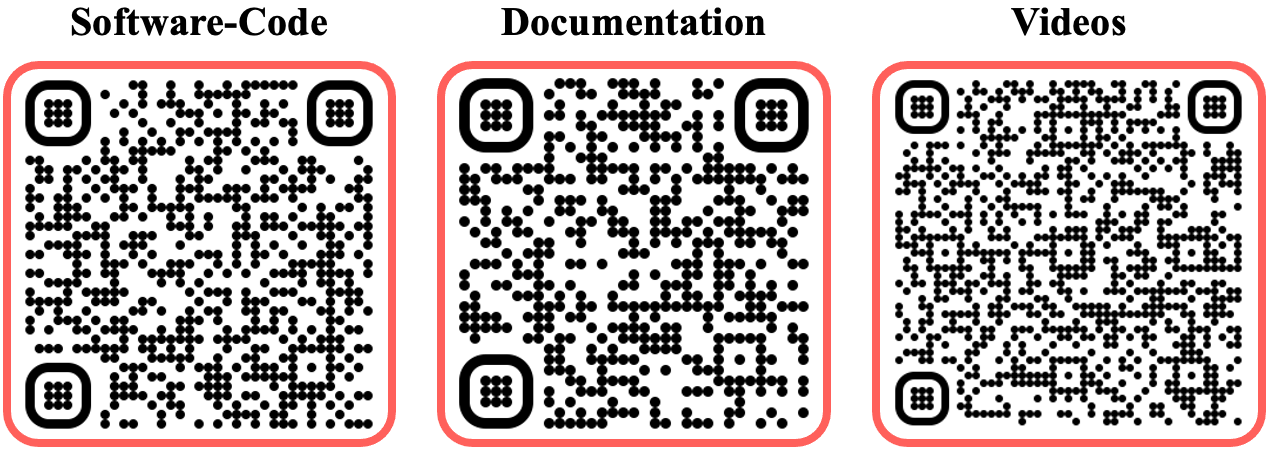
\includegraphics[width=0.79\textwidth]{qr_links}
    \caption[QR-Codes with links to sources]{QR-Codes with links to sources. The first code directs to the GitHub repository containing the source code, the second code to the repository containing the \LaTeX files to build this documentation, and the third code points to video visualisations of the results.}
    \figlbl{qr_links}
\end{figure}
%
The codebase and results from this thesis have been released as open source on GitHub: The code is available at \href{https://github.com/sagerpascal/lateral-connections}{github.com/sagerpascal/lateral-connections}, and the documentation is available at \href{https://github.com/sagerpascal/msc-thesis}{github.com/sagerpascal\\/msc-thesis}.
Furthermore, a GitHub webpage provides video visualisations from some of the results is available at \href{https://sagerpascal.github.io/lateral-connections/results/final_results.html}{sagerpascal.github.io/lateral-connections/results/final\_results}.
QR codes linking to these URLs are provided in \figref{qr_links} for convenient access using electronic devices.


\section{Video}\seclbl{result_video}
%
\begin{figure}[h]
    \centering
    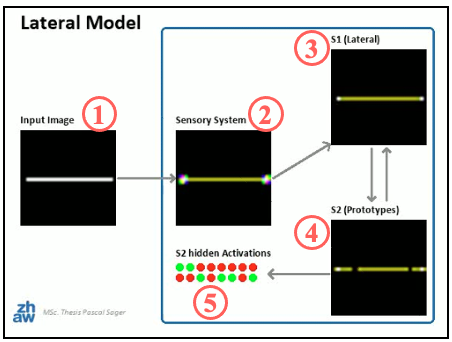
\includegraphics[width=0.99\textwidth]{video_overview}
    \caption[Overview of components visualised in the videos]{An overview of the components visualised in the videos.}
    \figlbl{video_overview}
\end{figure}
%
In the following, the video visualisations accessible at \href{https://sagerpascal.github.io/lateral-connections/results/final_results.html}{sagerpascal.github.io\\/lateral-connections/results/final\_results} are explained.
These explanations are limited to an overview of which components are shown in each video.
An interpretation of the video contents is provided in the corresponding result section.

Two video versions are shown for each experiment, both produced by the same model using the same parameter weights.
In the first video version, the Bernoulli neuron is replaced by a neuron using a fixed threshold.
This provides a video output that is more stable and has no flickering activations caused by sampling from a probability distribution.
For the \emph{S0} and \emph{S1} stages, a threshold of $0.5$ is used. Consequently, neurons with a probability of $\geq 0.5$ are set to $1$, while the other neurons are set to $0$.
A threshold of $0.9$ is used for the \emph{S2} stage, visualising only activities with high certainty that roughly correspond to those accepted by \emph{S1} as feedback signals.
The second video shows the network activities when the Bernoulli neurons are used.

Each video visualises the processing of the input over time.
The first six video frames show how the video is processed over the $T=6$ timesteps of the fast loop, followed by five additional frames depicting the final prediction after the fast loop.
By doing so, viewers have time to analyse the network's activations during this short interruption before the next input is fed into the model, and the process repeats.

\figref{video_overview} shows a single video frame, providing an overview of the components displayed in each video:
\begin{enumerate}
    \item The left part of the video displays the input image fed into the sensory system. It is a binary image with one colour channel, whereby active pixels are depicted in white and inactive pixels are depicted in black.
    \item The activations of the sensory system \emph{S0} are shown in the middle of the video. The sensory system extracts $4$ features at each location. Each feature combination is visualised in a different colour, and areas without activations are depicted in black.
    \item \emph{S1} is visualised in the top right corner. It uses the same colours as the sensory system. However, the activations might differ since neurons with insufficient lateral support are turned off, or other neurons might switch on.
    \item \emph{S2} is shown in the bottom right corner. It uses the same colours as the sensory system and \emph{L1}. The visualisation depicts the returned prototype, i.e., the feedback provided to \emph{S1} after mapping \emph{S1}' activities to the latent variables.
    \item The latent variables of \emph{S2} are shown at the center bottom of the video as $16$ circles. Each circle represents a cell, with green indicating an active cell and red indicating an inactive one. 
\end{enumerate}

For a detailed explanation of the content and observations in each video, please refer to the results chapter of this thesis.

\chapter{Negative Hebbian Learning}\chlbl{neg_hebb_updates}
%
\begin{figure}[h]
    \centering
    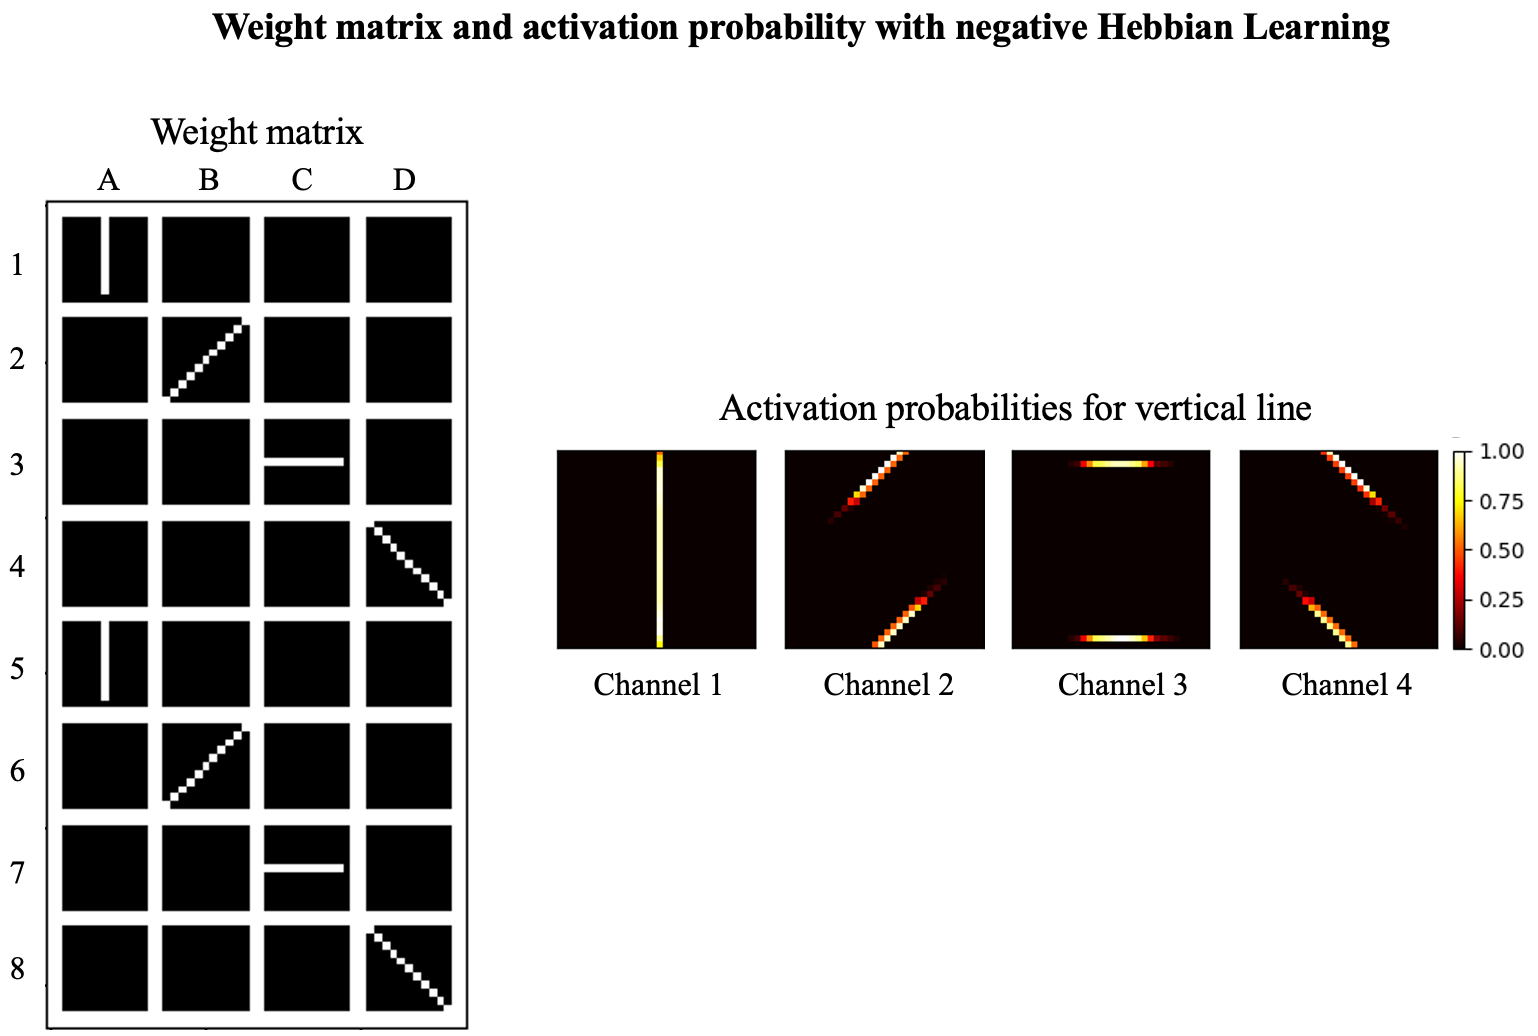
\includegraphics[width=0.99\textwidth]{neg_hebb_learning}
    \caption[Weight matrix and activations with negative Hebbian learning]{The weight matrix and the corresponding activation probabilities for a vertical line of a model trained with negative Hebbian learning.}
    \figlbl{neg_hebb_learning}
\end{figure}
%
This section examines the concept of negative Hebbian Learning in \emph{S1}, a learning paradigm designed to allow neural networks to forget unimportant or inconsistent features. 
In the conducted experiments, only positive Hebbian learning \sidecite{hebb_organization_1949} is used to strengthen connections between active cells.
Conversely, negative Hebbian learning additionally reduces the connection strength between cells that fire disjointly\sidenote{I.e. one cell is active while the other is inactive.}.
While negative Hebbian learning facilitates eliminating previously learned but inconsistent connections, it also poses challenges in maintaining desired lateral connections that are needed to provide support between feature cells.


\figref{neg_hebb_learning} visualises the weight matrix of a model trained with negative Hebbian updates and the activation probabilities if a vertical line fed is into the model.
Despite the divergence of the activation probabilities compared to those of positive Hebbian learning (c.f. \figref{S1_weight_analysis}), these activations are still considered valid representations of lines.
However, the major issue is that the output channels do not rely on multiple distinct features.

For instance, the output channel $A$ representing vertical lines only considers the input channels $1$ and $5$, whereby channel $1$ contains the ``vertical lines features'' from the sensory system, and channel $5$ is its own recurrent connection.
Regrettably, input channels $2$-$4$, which contain additional sensory signals, are disregarded by output channel $A$. Therefore, only cells representing vertical line features support this output channel.
In contrast, positive Hebbian learning considers all input channels, resulting in different features supporting each other.

Consequently, negative Hebbian learning leads to lower lateral support within the network.
This might not be an issue for the used line dataset but is crucial for real-world scenarios\sidenote{For example, one channel could represent eyes and another channel eyelashes. These features should support each other.}.
Negative Hebbian learning, while facilitating the filtering out of irrelevant features, also tends to make features mutually exclusive, which prevents learning adequate support between them.

\begin{figure}[h]
    \centering
    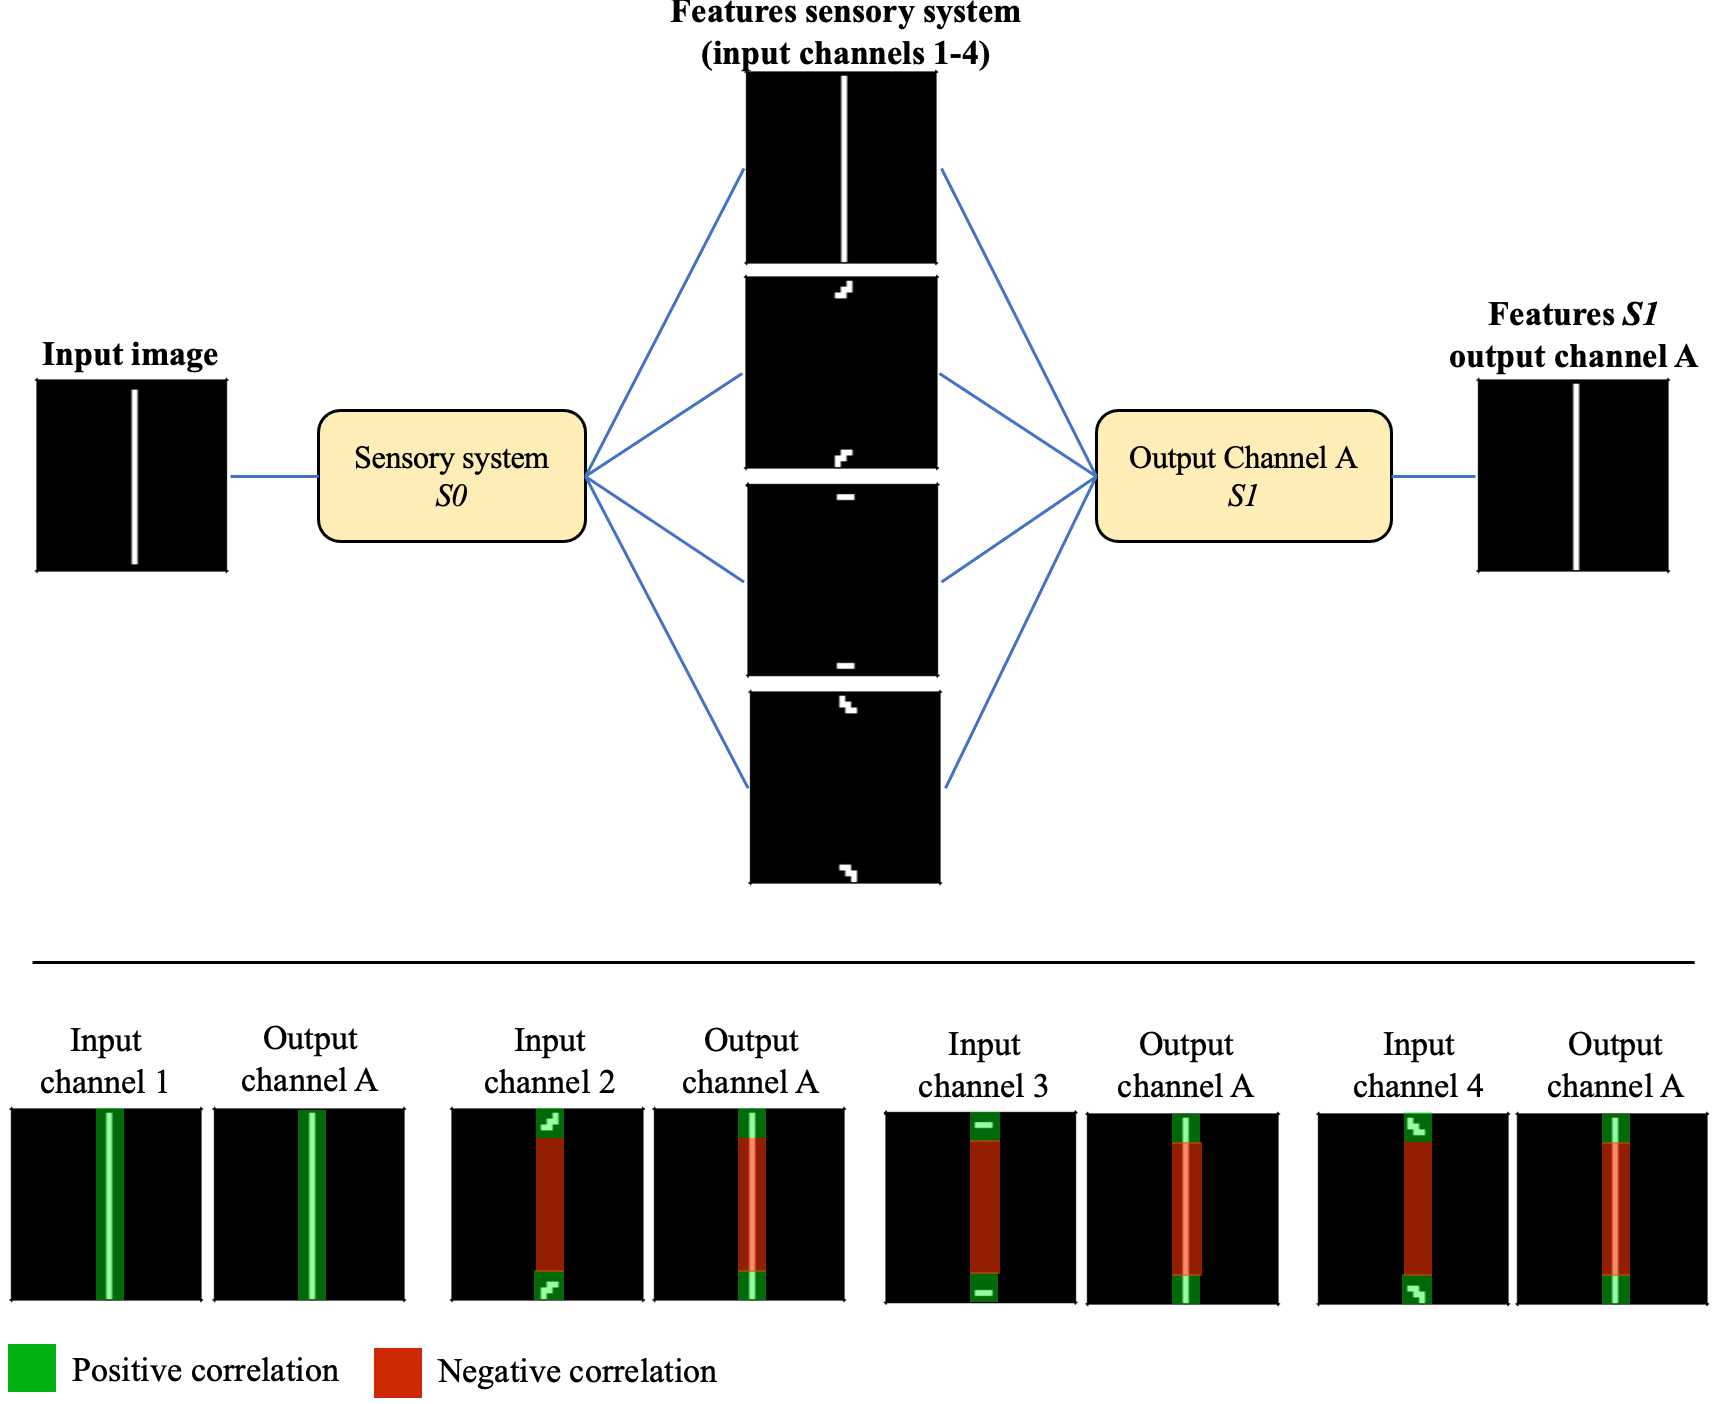
\includegraphics[width=0.99\textwidth]{correlations_hebb_learning}
    \caption[Feature correlation analysis]{Correlation between features from sensory input channels and the output channel $A$. The upper part of the images visualises the sensory features fed into output channel $A$ and the expected result. The lower part of the image indicates where positive and negative correlation occurs between sensory channels and output channel $A$.}
    \figlbl{correlations_hebb_learning}
\end{figure}
%
The primary issue is that, except for one input channel, there are more negative correlations between the input channels and a single output channel, as illustrated in \figref{correlations_hebb_learning}.
In this context, ``negative correlation'' refers to disjointly active cells, while ``positive correlation'' refers to cells that fire together.
In the case of the vertical line, the output channel $A$ is expected to reassemble the line roughly.

Hebbian learning compares this output with the input channels, strengthening the weights for positively correlated input-output pairs and weakening them for negatively correlated pairs.
These correlations are visualised in the lower part of \figref{correlations_hebb_learning}.
Input channel $1$ and output channel $A$ have high similarity. Therefore, the activations between input and output have a positive correlation, and the corresponding lateral connections undergo a positive Hebbian update.
However, all the other channels have a positive correlation only at the line ends and a negative correlation in the middle section of the line.
Consequently, there is more negative than positive correlation, and these features undergo more negative than positive updates.
This causes the lateral support learned at the line ends to be suppressed by the negative updates triggered by the negative correlation in the middle of the line.

The resolution to this issue remains unclear and requires additional experiments. One potential approach is to use a significantly lower learning rate for negative updates than for positive updates; another solution could be to introduce alternative cells (c.f. \secref{future_alt_cells})




%%%%%%%%%%%%%%%%%%%%%%%%%%%%%%%%%%%%%%%%%%%%%%%%%%%%%%%%%%%%%%%%%%%%%%%%%%%%%%%%
%%%%%%%%%%%%%%%%%%%%%%%%%%%%%%%%%%%%%%%%%%%%%%%%%%%%%%%%%%%%%%%%%%%%%%%%%%%%%%%%
\backmatter
\setchapterstyle{plain}


%%%%%%%%%%%%%%%%%%%%%%%%%%%%%%%%%%%%%%%%%%%%%%%%%%%%%%%%%%%%%%%%%%%%%%%%%%%%%%%%
\defbibnote{bibnote}{Here is the list of references in citation order.\par\bigskip}
\printbibliography[heading=bibintoc, title=Bibliography, prenote=bibnote]


%%%%%%%%%%%%%%%%%%%%%%%%%%%%%%%%%%%%%%%%%%%%%%%%%%%%%%%%%%%%%%%%%%%%%%%%%%%%%%%%
\printindex


%%%%%%%%%%%%%%%%%%%%%%%%%%%%%%%%%%%%%%%%%%%%%%%%%%%%%%%%%%%%%%%%%%%%%%%%%%%%%%%%
%\clearpage
%\thispagestyle{empty}
%\null%
%\clearpage
%\includepdf{cover-back.pdf}

%%%%%%%%%%%%%%%%%%%%%%%%%%%%%%%%%%%%%%%%%%%%%%%%%%%%%%%%%%%%%%%%%%%%%%%%%%%%%%%%
\end{document}
%%%%%%%%%%%%%%%%%%%%%%%%%%%%%%%%%%%%%%%%%%%%%%%%%%%%%%%%%%%%%%%%%%%%%%%%%%%%%%%%
